\chapter{Поисковые методы идентификации}

\section{Критерии идентификации} % {{{1 _criteria_

\subsection{Свойства и параметры критериев идентификации} % {{{2

Особливість динаміки хаотичних систем не дозволяє визначити мету ідентифікації
як задачу мінімізації будь-якої міри
$\mu(x_o(t), x_i(t))$ у просторі вихідних
сигналів~\cite{atu_asau11,atu_asau12,atu_asau14,atu_electronika2013}.


На рис.~\ref{atu:f:lor_diff_x0} приведён пример, показывающий
различие траекторий для системы Лоренца~\cite{moon_chaotic_vibr}
при малом возмущении значений начальных условий.
Относительная разница в начальном значении переменной состояния $x_0$
составляет~$1\times 10^{-8}$.

\begin{figure}[htb!]
  \centerline{
    \includegraphics[width=0.49\textwidth]{p/lor_diff-p_xx_x0.png}
    \hfill
    \includegraphics[width=0.49\textwidth]{p/lor_diff-p_dx_x0.png}
  }
  \caption{Различие в поведение системы Лоренца при малом возмущении начальных условий}
  \label{atu:f:lor_diff_x0}
\end{figure}


На рис.~\ref{atu:f:lor_diff_sigma} приведён пример, показывающий
различие траекторий для системы Лоренца
при малом возмущении значений параметра $\sigma$,
которое составляет в относительных единицах~$1 \times 10^{-9}$.

\begin{figure}[htb!]
  \centerline{
    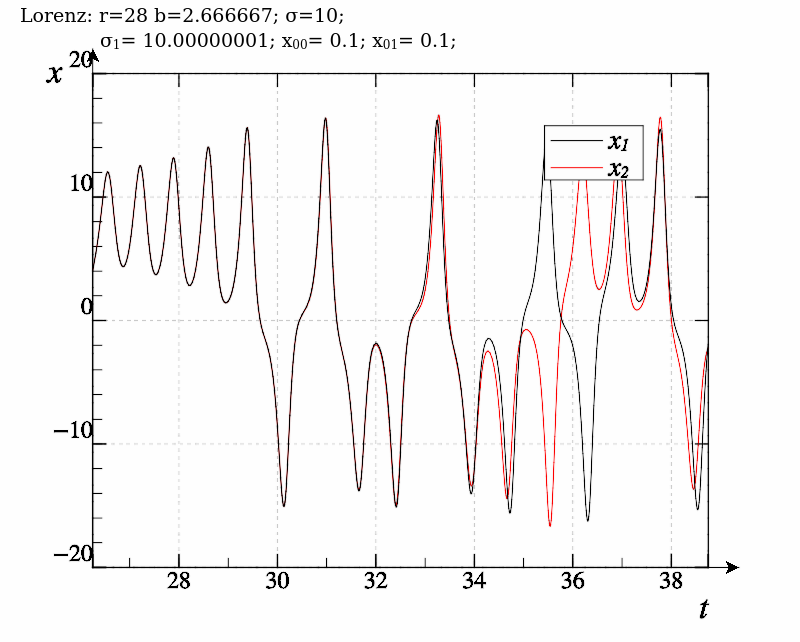
\includegraphics[width=0.49\textwidth]{p/lor_diff-p_xx_sigma.png}
    \hfill
    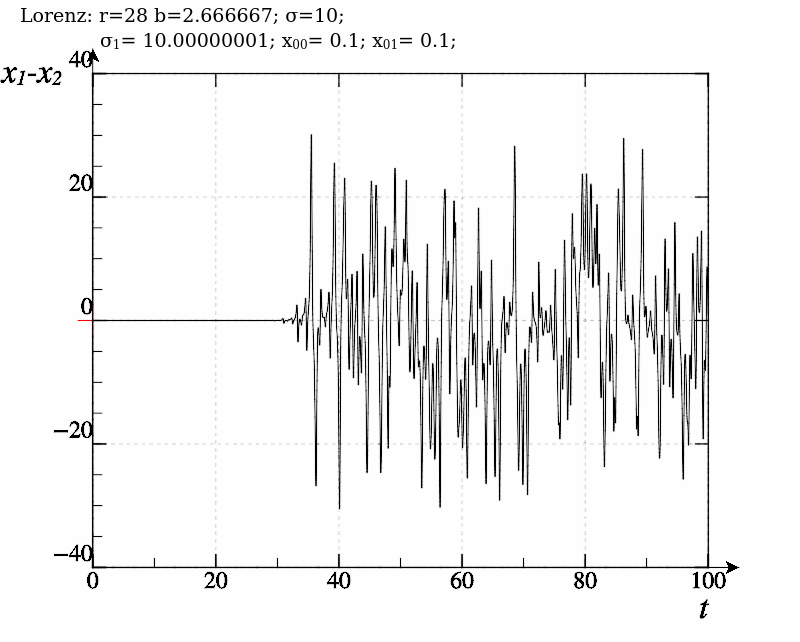
\includegraphics[width=0.49\textwidth]{p/lor_diff-p_dx_sigma.png}
  }
  \caption{Различие в поведение системы Лоренца при малом возмущении параметра $\sigma$}
  \label{atu:f:lor_diff_sigma}
\end{figure}

Эти примеры, демонстрирующие чувствительность фазовых траекторий хаотических систем
как к пренебрежимо малым изменениям параметров, так и к малым изменениям
в состоянии системы, подчёркивают тот факт, что близость
(или даже совпадение, при условии различной истории) параметров модели
и объекта не обозначает близость фазовых траекторий систем
в смысле наиболее часто используемых мер функциональных пространств.
Более того, ввиду плотного заполнения аттракторов таких систем
можно подобрать достаточно близкие траектории для систем с различными значениями параметров
на ограниченном интервале времени.

Отже, для синтезу системи ідентифікації необхідно існування заданого скалярного
критерію $q(x(t))$, близькість величин якого для об'єкта і моделі (в сенсі
будь-якої міри) і дозволяє говорити про досягнення мети ідентифікації~\cite{crit_method_is}.


Для створення можливості використання критерію для цілей ідентифікації
динамічних системи, сам критерій повинен якимось чином відображати глобальні
властивості системи, а не її стану в конкретний момент часу, тобто не
змінюватися (принаймні істотно), якщо властивості системи, що пред'являються в
математичні моделі параметрами, не змінюються. У таких випадках має сенс
використовувати термін ``інтегральні критерії''.

Існує множина засобів визначення
критеріїв~\cite{atu_asau11,atu_asau12,atu_asau14,atu_khar_autodor25,atu_asau18,atu_st79,atu_apir2013}.
Для досить простих систем вид критерію, придатного для задачі ідентифікації,
можна вивести, визначивши будь-яким чином виходячи зі структури математичної
моделі. У деяких випадках вид критерію можна підібрати емпірично, на
підставі досвіду в синтезі систем ідентифікації для подібних систем~\cite{atu_asau24}. Проте,
найбільш обґрунтованим є підхід, заснований на використанні будь-яких фізичних
інваріантів.



Практически в каждом разделе физики существуют
определённые законы сохранения.
Прежде всего стоит назвать общеизвестные и всеобщие
законы сохранения энергии, импульса, момента импульса.
Также существуют и применяются законы сохранения
электрического, лептонного и барионного зарядов,
принцип бесцветности и~т.д~\cite{vigner_invar}.

Найбільш загальним, і, отже, найбільш вживаним є закон збереження енергії.

Помимо закона сохранения энергии, существуют области,
где имеет смысл применять другие, вплоть до синтетических
законов сохранения, но этот подход
применяется реже.

Каждый из законов сохранения является инвариантом,
и может служить для синтеза критерия в какой-либо области
при определённых условиях.
Тем не менее, непосредственно применение
физических законов сохранения не всегда
удобно и прямолинейно.
Например, в теории управления системы динамического
хаоса относят к ``диссипативным'' системам.
Сам этот термин несколько отличается от аналогичного,
применяемого в физике.
Там система считается диссипативной, если она не
получает энергию извне, а имеющуюся переводит
в не описываемую рассматриваемым комплексом взаимодействий
форму, чаще всего в тепло. \Cmt{ref}
В теории управления
считается, что система, сохраняя процесс диссипации
(перевода энергии в неконтролируемую форму),
получает энергию извне, что и обеспечивает её незатухающую
динамику~\cite{prigogine_selforganization,chernavskii_syn_info,prigogine_order_from_chaos}.
Более того, сам вид уже существующих
математических моделей хаотических систем не позволяет
явно выделить понятие энергии в чистом виде.
В таких случаях
приходится прибегать к полуэмпирическим методам,
рассматривая доступные переменные состояния системы,
проводя анализ их влияния и, в результате моделирования,
выбирая подходящий вид критерия.


Розглянемо основні способи подання енергії:

кінетична енергія тіла масою $m$, яке рухається зі швидкістю $v$:
%
\begin{equation}
  E_k = \frac{mv^2}{2} = \frac{m}{2} \left( \od{x}{t} \right)^2.
  \label{atu:eq:Ek_v}
\end{equation}
%
Следует обратить внимание, что, по сравнению с классическим
представлением энергии при обработке сигналов,
здесь присутствует квадратичная зависимость от производной сигнала.

Потенційна енергія в однорідному полі (нульовий рівень обирається довільно):
%
\begin{equation}
  E_p = m g x .
  \label{atu:eq:Ep_g}
\end{equation}

Потенційна енергія в пружному наближенні:
%
\begin{equation}
  E_p = k \frac{x^2}{2} .
  \label{atu:eq:Ep_spring}
\end{equation}

Кінетична енергія тіла, що обертається:
%
\begin{equation}
  E_k = J \frac{\omega^2}{2} = \frac{J}{2} \left( \od{\varphi}{t} \right)^2 .
  \label{atu:eq:Ek_spin}
\end{equation}

Внутрішня теплова енергія:
%
\begin{equation}
  E_t = \frac{im}{2M} RT.
  \label{atu:eq:Et}
\end{equation}

Електрична енергія, накопичена в конденсаторі:
%
\begin{equation}
  E_c = \frac{C U^2}{2}.
  \label{atu:eq:Ec}
\end{equation}

Енергія магнітного поля, накопичена в котушці індуктивності:
%
\begin{equation}
  E_l = \frac{L I^2}{2} = \frac{L}{2} \left( \od{Q}{t}\right)^2 .
  \label{atu:eq:El}
\end{equation}

Енергія, яка перетворюється у тепло омічним опором:
%
\begin{equation}
  E_r = U I = I^2 R = \frac{U^2}{R} = U \od{Q}{t} .
  \label{atu:eq:Er}
\end{equation}


% \Cmt{Chemical kinetic -- $\max(x)$}.
%
% \Cmt{Electro-magnetic -- $x\cdot y$}.


Узагальнюючи вищезазначене, можна зробити висновок, що, незважаючи на
різноманітність фізичних процесів, кількість способів подання енергії
(розглядаємо зосереджені параметри) досить обмежена. Основні види залежностей:

\begin{itemize}

  \item
    Квадратичная зависимость от координаты:
    $E \sim x^2$.

  \item
    Лінійна залежність від координати:
    $E \sim x$.

  \item
    Квадратична залежність від похідної координати за часом:
    $E \sim \left( \od{x}{t}\right)^2$.

  \item
    Лінійна залежність від добутку координат:
    $E \sim x \cdot y$.

  \item
    Лінійна залежність від добутку однієї координати на похідну іншої:
    $E \sim x \cdot \od{y}{t}$.

  \item
  Максимум величини на заданому інтервалі часу.

\end{itemize}

Таким образом, в тех случаях, когда нет возможности
использовать явный, непосредственно вытекающий
из строгого анализа системы критерий, в качестве кандидатов
имеет смысл перебрать возможные комбинации из перечисленных выражений.
При этом следует учитывать, что, в отличие от строгих законов сохранения
полученные величины характеризуют систему (или её отдельные элементы)
в достаточно грубом приближении.
Ещё одним важным отличием критериев, построенных по такой схеме,
от строгих законов сохранения является то,
что законы сохранения выполняются строго в каждый момент
(с точностью, обеспечиваемой измерениями). Напротив,
критерии, полученные таким полуэмпирическим путём,
имеют смысл только после какого-либо усреднения.








Следствием невозможности непосредственного использования выходных
сигналов объекта и моделей в качестве критерия идентификации, а также
требование физической измеримости критерия является
тот факт, что для получения оценки критерия, как правило,
требуется значительное время~\cite{atu_ich2011,atu_DSMP2016}. % TODO: more ref






% Монотонность -- как следствие одноэкстремальность?


%Зависимость (обозначение?) от времени оценивания.
%Методы измерения.



% }}}2


\subsection{Отличие задачи идентификации от задач решения нелинейного уравнения и поиска экстремума} % {{{2

% \Cmt{Перенести куда-то}

На перший погляд, при заданому критерії ідентифікації, задача ідентифікації
зводиться до класичної задачі розв'язання нелінійного рівняння: треба знайти
такі значення параметрів $p$, при яких критерій моделі (або будь-якої з
моделей) $q_m$ приймає значення, найбільш близьке до значення критерію
об'єкта $q_o$:
\[
  \mu( q_o, q_m(p) ) \to \min.
\]
%
Или же при использовании функции качества идентификации $F(q_o, q_m )$ задача
эквивалентна классической задаче поиска экстремума:
\[
  \overline{F}( q_o, q_m(p) ) \to \max.
\]
%
Насправді, існують певні аспекти, які роблять таке зведення практично
неможливим.

Перш за все, в завданню в обох вихідних задачах передбачається, що
спостережувана система статична: значення критерію не залежить від часу, і
провівши вимір в точці один раз, можна до нього не повертатися. Навпаки,
ідентифікація динамічної системи передбачає, що значення критерію, навіть після
будь-якого усереднення на кінцевому інтервалі часу, є величина динамічна,
причому динаміка визначається не тільки параметрами системи, але і
властивостями самої системи вимірювання, а також процесом взаємодії системи
вимірювання з моделями. При цьому можливі досить нетривіальні явища, такі як
параметричний резонанс~\cite{landau1}, поширення параметричних хвиль на множині моделей.

Также существенную роль могут играть как шумы измерения, так и побочные
эффекты от процесса фильтрации шумов.
Применение практически любого фильтра приводит к запаздыванию
в процессе измерения, и игнорирование этих явлений может привести
как к нарушению устойчивости поиска, так и получению совершенно
неадекватных результатов при наличии устойчивости.

В исходных задачах предполагается, что не только
значение функции известно точно в каждой точке, но также известны все производные
(по крайней мере, необходимые для работы метода).
В реальные задачах идентификации производные непосредственно
не доступны для измерения, а их оценка требует применения специальных
методов. При этом процесс оценивания производных, как правило,
более чувствителен к шумам измерения, чем собственно измерение.


% \Cmt{ TODO: Требование конечности производных в условиях дискретного представления сигнала.}

Все эти явления делают задачу идентификации более сложной, чем
исходные задачи, чем и обусловлено
существование широкого спектра методов идентификации. Тем не менее,
некоторые алгоритмы, применимые при поиска экстремума, могут быть
полезны при синтезе системы идентификации.

% Свёртка с чем-то.

Поняття інтегрального критерію, що застосовується до реальних задач, передбачає
не тільки взяття або оцінку інтеграла та обраному часовому
інтервалі, а й нормування на величину цього інтервалу. Це дає можливість
застосованим критеріям не мати явної мультиплікативної залежності від часу, і
описувати властивості саме об'єкта. Таким чином, інтегральний критерій можна
уявити як різновид усереднення для виразу, що формує цей критерій.

Однако, такие виды усреднения, как среднее арифметическое, медиана и т.д.
неприменимы для формирования критерия для систем с изменяющимся параметром.
Для реализации возможности такого определения необходимо ограничить
по времени усредняемый диапазон.
Оценку этого ограничения обозначим
\label{atu:d:tau_q}$\tau_q$.
В какой-то мере это эквивалентно
применению фильтра нижних частот с частотой среза
\label{atu:d:a_q}$a_q = 1 / \tau_q$.
Рассмотрим возможные реализации такого усреднения.

Найбільш очевидний спосіб обмеженого за часом усереднення ---
ковзне середнє~\cite{greshilov_mat_met_prognoz}.
Якщо базовий вираз для формування критерію позначити як
$x(t)$, то цей спосіб усереднення має вигляд:
%
\begin{equation}
  q_{x,a}(t) =
  \frac{1}{\tau_q}
  \int\limits_{t-\tau_q}^{t} x(t) \, dt.
  \label{atu:eq:moving_avarage}
\end{equation}

Суффиксом ``,a'' в определении критерия будем обозначать
именно это определение.
Несмотря на простоту определения, хорошие частотные характеристики,
применения этого метода в реальных задачах довольно неудобно.
Прежде всего, при численной реализации такого интегрирования
необходимо хранить большое количество предыдущих значений,
алгоритмически обеспечить корректный старт при $\tau_q$.
Также при реализации этого метода эффективным алгоритмом,
при котором количество операций на каждом шагу не зависит от $\tau_q$,
возникают вопросы накопления ошибок вычисления.

Менш витратним (з точки зору обсягу обчислень) є метод експоненціального
згладжування, динаміку якого стосовно сигналу $x(t)$ можна описати
рівнянням:
%
\begin{equation}
\od{q_{x,l}}{t}
=
\frac{1}{\tau_q} \left( x(t) - q_{x,l}(t) \right)
\label{atu:eq:qlin}
\end{equation}

Суффикс ``,l'' в дальнейшем изложении будет применяться
для усреднения вида~(\ref{atu:eq:qlin}).
Численная реализация подобного сглаживания не представляет
проблем. Существуют эффективные, в том числе аппаратные
реализации (\ref{atu:eq:qlin}) в дискретном представлении (БИХ-фильтры).
Также возможно, в случае наличия информации о спектральном составе $x(t)$
применении более сложных фильтров для задачи усреднения.
Однако, при идентификации хаотических систем непрерывность спектра
будет препятствовать применению эффективных фильтров.


Если $q(x(t))$  --- подходящий для задачи идентификации критерий,
причём $x(t)>0 \forall t>0$,
$f(x)$ --- строго монотонная функция $\forall x > 0 $,
то и $q(f(x(t))$ --- тоже подходящий для рассматриваемой задачи критерий.
Тем не менее, близость полученной интегральной зависимости в стационарном случае $q(p)$
к линейной позволяет системе идентификации функционировать в близких режимах
на всей области определения~$p$. Для достижения этой цели
при выборе вида критерия следует, если это возможно,
использовать физические соображения для приближения к линейной зависимость $q(p)$,
или же, использовать перебор для выбора наиболее подходящего определения.
С учетом (\ref{atu:eq:Ek_v})--(\ref{atu:eq:Er}) приведём
примеры подобных определений.


\begin{equation}
\od{q_{x^2,l}}{t}
=
\frac{1}{\tau_q} \left( x^2(t) - q_{x^2,t}(t) \right)
,
\label{atu:eq:qx2l}
\end{equation}

\begin{equation}
  q_{xr,a}(t) =
  \sqrt{
    \frac{1}{\tau_q}
    \int\limits_{t-\tau_q}^{t} x^2(t) \, dt
  }.
  \label{atu:eq:qxra}
\end{equation}

\begin{equation}
  q_{|x|,a}(t) =
  \frac{1}{\tau_q}
  \int\limits_{t-\tau_q}^{t} |x|(t) \, dt
  .
  \label{atu:eq:qxma}
\end{equation}

\begin{equation}
  q_{xy^{0.5},a}(t) =
  \sqrt{
    \frac{1}{\tau_q}
    \int\limits_{t-\tau_q}^{t} x(t)y(t) \, dt
  }
  .
  \label{atu:eq:qxy05a}
\end{equation}

При этом следует отметить, что в стационарном случае, при значительных величинах $\tau_q$,
различные методы усреднения дают практически неразличимые результаты, и зависимости
как от $\tau_q$, так и от $t$ становятся пренебрежимо малыми.
Получившуюся зависимость от параметра объекта будем обозначать $q(p)$.


% }}}2

% TODO dynamic q props

% }}}1 _criteria_

\section{Основные понятия и параметры поисковых систем идентификации}  % {{{1

\subsection{Априорная и текущая информация}  % {{{2

Без апріорної інформації неможлива побудова працездатною системи ідентифікації.

Основні апріорні величини визначаються на етапі постановки задачі
ідентифікації.
Частину апріорної (по відношенню до ідентифікації) інформації
надає процес синтезу критерію ідентифікації. В першу чергу, це сам вид
критерію. Їм визначаться як діапазон зміни величини цього критерію
$\Delta q$, так і динамічні властивості: залежності
$\sigma_q (\tau_q)$ або $\sigma_q(a_q)$,
в найпростіших випадках, при заданій точності --- характерний або
мінімальний час оцінювання ($\tau_{q, \min}$),
характерний час реакції
системи $\tau_p$ на зміну параметра з урахуванням динаміки вимірювання $(q)$.

Без априорной информации невозможно построение
работоспособной системы идентификации. Основные
априорные величины определяются на этапе постановки
задачи идентификации. В первую очередь это
параметры масштаба: множество допустимых
значений параметров \label{atu:d:p_set}\( \mathcal{P}\),
характерное время работы
идентифицируемой системы~$T$, а также
требуемая точность и скорость идентификации
(могут быть заданы различными способами).
В этот список может входить и ограничения на динамику изменения параметра.
В процессе работы эти параметры могут уточнятся по текущей информации.

Следующую часть априорной (по отношению к идентификации) информации
предоставляет процесс синтеза критерия идентификации.
В первую очередь, это сам вид критерия. Им определятся
как диапазон изменения величины этого критерия $\Delta q$, так и
динамические свойства:
зависимости $\sigma_q(\tau_q)$ или  $\sigma_q(a_q)$,
в простейших случаях, при заданной точности --- характерное/минимально время
оценивания \(\tau_{q,\min}\),
характерное время реакции системы $\tau_p$ на изменение
параметра с учётом динамики измерения \(q\).

Процес пошукової ідентифікації полягає в налаштовуванні параметрів однієї або
декількох моделей, визначення критеріїв ідентифікації і відповідних функцій
якості, і оцінювання за цією інформацією значення ідентифікованого параметра
\label{atu:d:p_id}$p_\mathrm{id}$. При використанні в цілях
ідентифікації декількох моделей, з'являються спільні дії, що застосовуються до
кожної з них.


% }}}2


\subsection{Функции качества идентификации и безразмерный вид критерия}  % {{{2


Критерій, заснований на фізичних принципах, найчастіше є розмірною величиною.
Навіть у тому разі, коли конкретний вид критерію визначено емпірично або
підбором, критерій найчастіше є розмірною величиною.
Як наслідок, безпосереднє
використання величини критерію досить незручно. Наприклад, при зміні одиниць
виміру, зміні загального масштабу об'єкта, значення такого критерію також
будуть зміняться, що досить незручно при синтезі системи ідентифікації.

Вторая проблема вызвана тем, что ни существование достаточно
адекватной модели, ни построение хорошего критерия качества идентификации
не даёт возможность ответить на вопрос о качестве результата,
полученного в процессе работы системы идентификации.
Необходимо внешнее условие, позволяющее оценить полученный результат.
Сравнение в пространстве параметров допустимо практически только для
искусственных модельных задач. Следовательно,
должен быть каким-либо образом задан характерный масштаб
в пространстве критериев, определяющий полученное качество
идентификации.

Есть, как минимум, два подхода к решению данной проблемы.
Первый достаточно очевиден --- все критерии приводятся к безразмерному виду путём деления
на какую-либо характерную величину той же размерности. В качестве такой величины
можно взять максимальное значение критерия при текущих ограничениях,
значение критерия для ``центральной'' точки множества $\mathcal{P}$,
а также подходящую по смыслу и размерности величину, полученную
из анализа физических размерностей.
При этом требуемое качество идентификации задаётся в
выбранных безразмерных единицах.

Второй подход используется при создании экстремальных систем управления
Другий метод використорується при створенні екстремальних систем управління --- введення ``функції якості''.
% \Cmt{TODO: ref.}

При использовании введённых обозначений для задачи идентификации
определим её следующим образом:
\label{atu:d:F}$F(q_o, q_m)$.
На цю функцію накладається наступни умови:

\begin{itemize}

  \item
    Інваріантність по відношенню до зсуву:
    $F(a+c,b+c) = F(a,b)$.
    Невыполнение этого требования обозначает зависимость метода
    от используемой системы координат, и, как следствие --- приводит к логической
    противоречивости метода.
    Если в этом условии положить $c = -b$, то
    очевидно, что для определении функции $F(a,b)$ 
    с двумя аргументами достаточно определить функцию
    с одним аргументом: $ F(a-b,b-b) = F(a-b,0) = F(a-b)$.

  \item
    Симетричність: $ F(a,b) = F(b,a)$ или же $F(a) = F(-a)$,
    что эквивалентно заданию функции как $F(|a|)$.
    Наличие этого требования обусловлено потребностью в получении несмещённых
    оценок идентифицируемого параметра.

  \item
    існування одного екстремуму
    с определенным значением, для определённости единичным:
    $F(a,b) = 1  \Leftrightarrow a = b $.
    Или же в представлении функции с одним аргументом $F(0) = 1$.
    Наличие нескольких экстремумов делает результат процесса идентификации неоднозначным.
    Это требование совершенно не налагает требование одноэкстремальности
    на функцию $F(q(p_m), q(p_o)), \; p_o = \mathrm{const}$. Тем не менее, при
    монотонной зависимости $q(p)$ это будет выполнятся автоматически.

  \item
    Монотонність на кожної з гілок:
    если $ a_2-b_2 > a_1-b_1, \; a_i-b_i \ge 0$, то $F(a_1,b_1) \ge F(a_2,b_2)$.
    Нарушение этого условия также может привести к нарушению процесса поиска,
    так как при этом вносятся искусственные локальные экстремумы.
    При этом условие $F(a_1,b_1) = F(a_2,b_2)$ допустимо только в удалении от
    рабочей области. Вариант с одним аргументом:
    $ a_2 > a_1, a_1 \ge 0 \to F(a_1) \ge F(a_2)$.

  \item
   Неперервність ---
    используется классическое определение из математического анализа.
    Формально это требование не является строго обязательным, многие из рассмотренных
    в работе методов могут сохранить работоспособность и в этом случае. Тем не менее,
    не следует без особой необходимости создавать искусственные помехи нормальному функционированию
    системы идентификации.

\end{itemize}

Эти требования при применении на практике часто дополняются
требованием к простоте реализации функции качества,
или даже к возможности её схемотехнической реализации
без применения элементов вычислительной техники.
 % легкість схемотехнічної реалізації.

Для удобства использования различных функций качества
в одной и той же системе идентификации, а также для
упрощения сравнения свойств исследуемых методов,
примем:
\begin{equation}
  F(a,a) = 1;
  \quad
  \lim\limits_{b \to \pm \infty } F(a,b) = 0.
  \label{atu:eq:F_scale}
\end{equation}




С учётом обозначения
\begin{equation}
  q_r = \frac{q_o - q_m}{q_\gamma},
\label{atu:eq:q_r}
\end{equation}
%
\noindent
отображающего тот факт, что первым этапом построения функции качества
является приведение к безразмерному виду,
представлены наиболее распространённые виды таких функций~\cite{atu_ISDMCI2016,atu_asau24}:
%
\begin{equation}
  F_{\mathrm{gauss}} = \exp( - q_r^2 ),
\label{atu:eq:F_gauss}
\end{equation}
%
\begin{equation}
  F_{\mathrm{parabolic}} = 1 - q_r^2 \left( 1 - \frac{1}{e} \right),
\label{atu:eq:F_parabolic}
\end{equation}
%
\begin{equation}
  F_{\mathrm{triangle}} = 1 - |q_r| \left( 1 - \frac{1}{e} \right),
\label{atu:eq:F_triangle}
\end{equation}
%
\begin{equation}
  F_{\mathrm{hyper}} = \frac{1}{ 1 + |q_r| \left( 1 - \frac{1}{e} \right)},
\label{atu:eq:F_hyper}
\end{equation}
%
\begin{equation}
  F_{\mathrm{log}} = 1 - \ln \left( 1 + |q_r| \right) \frac{1-1/e}{\ln(2)}.
\label{atu:eq:F_log}
\end{equation}

Для всех рассмотренных функций $q_\gamma$ --- величина, обратная чувствительности
функции качества, задаёт масштаб и рабочий диапазон функции качества (рис.~\ref{atu:f:F_types}).
Для усіх розглянутих функцій $q_\gamma$ --- величина,
яка, задає масштаб і робочий діапазон функції якості.
При этом, как правило, значения этих функций могут быть искусственно ограничены диапазоном $[0;1]$.
Каждая из рассматриваемых функций имеет свой набор преимуществ и недостатков~\cite{atu_ISDMCI2016}.
Подробнее этот вопрос будет рассмотрен в главе~\ref{atu:ch:testsys}.

\begin{figure}[htb!]
  \centerline{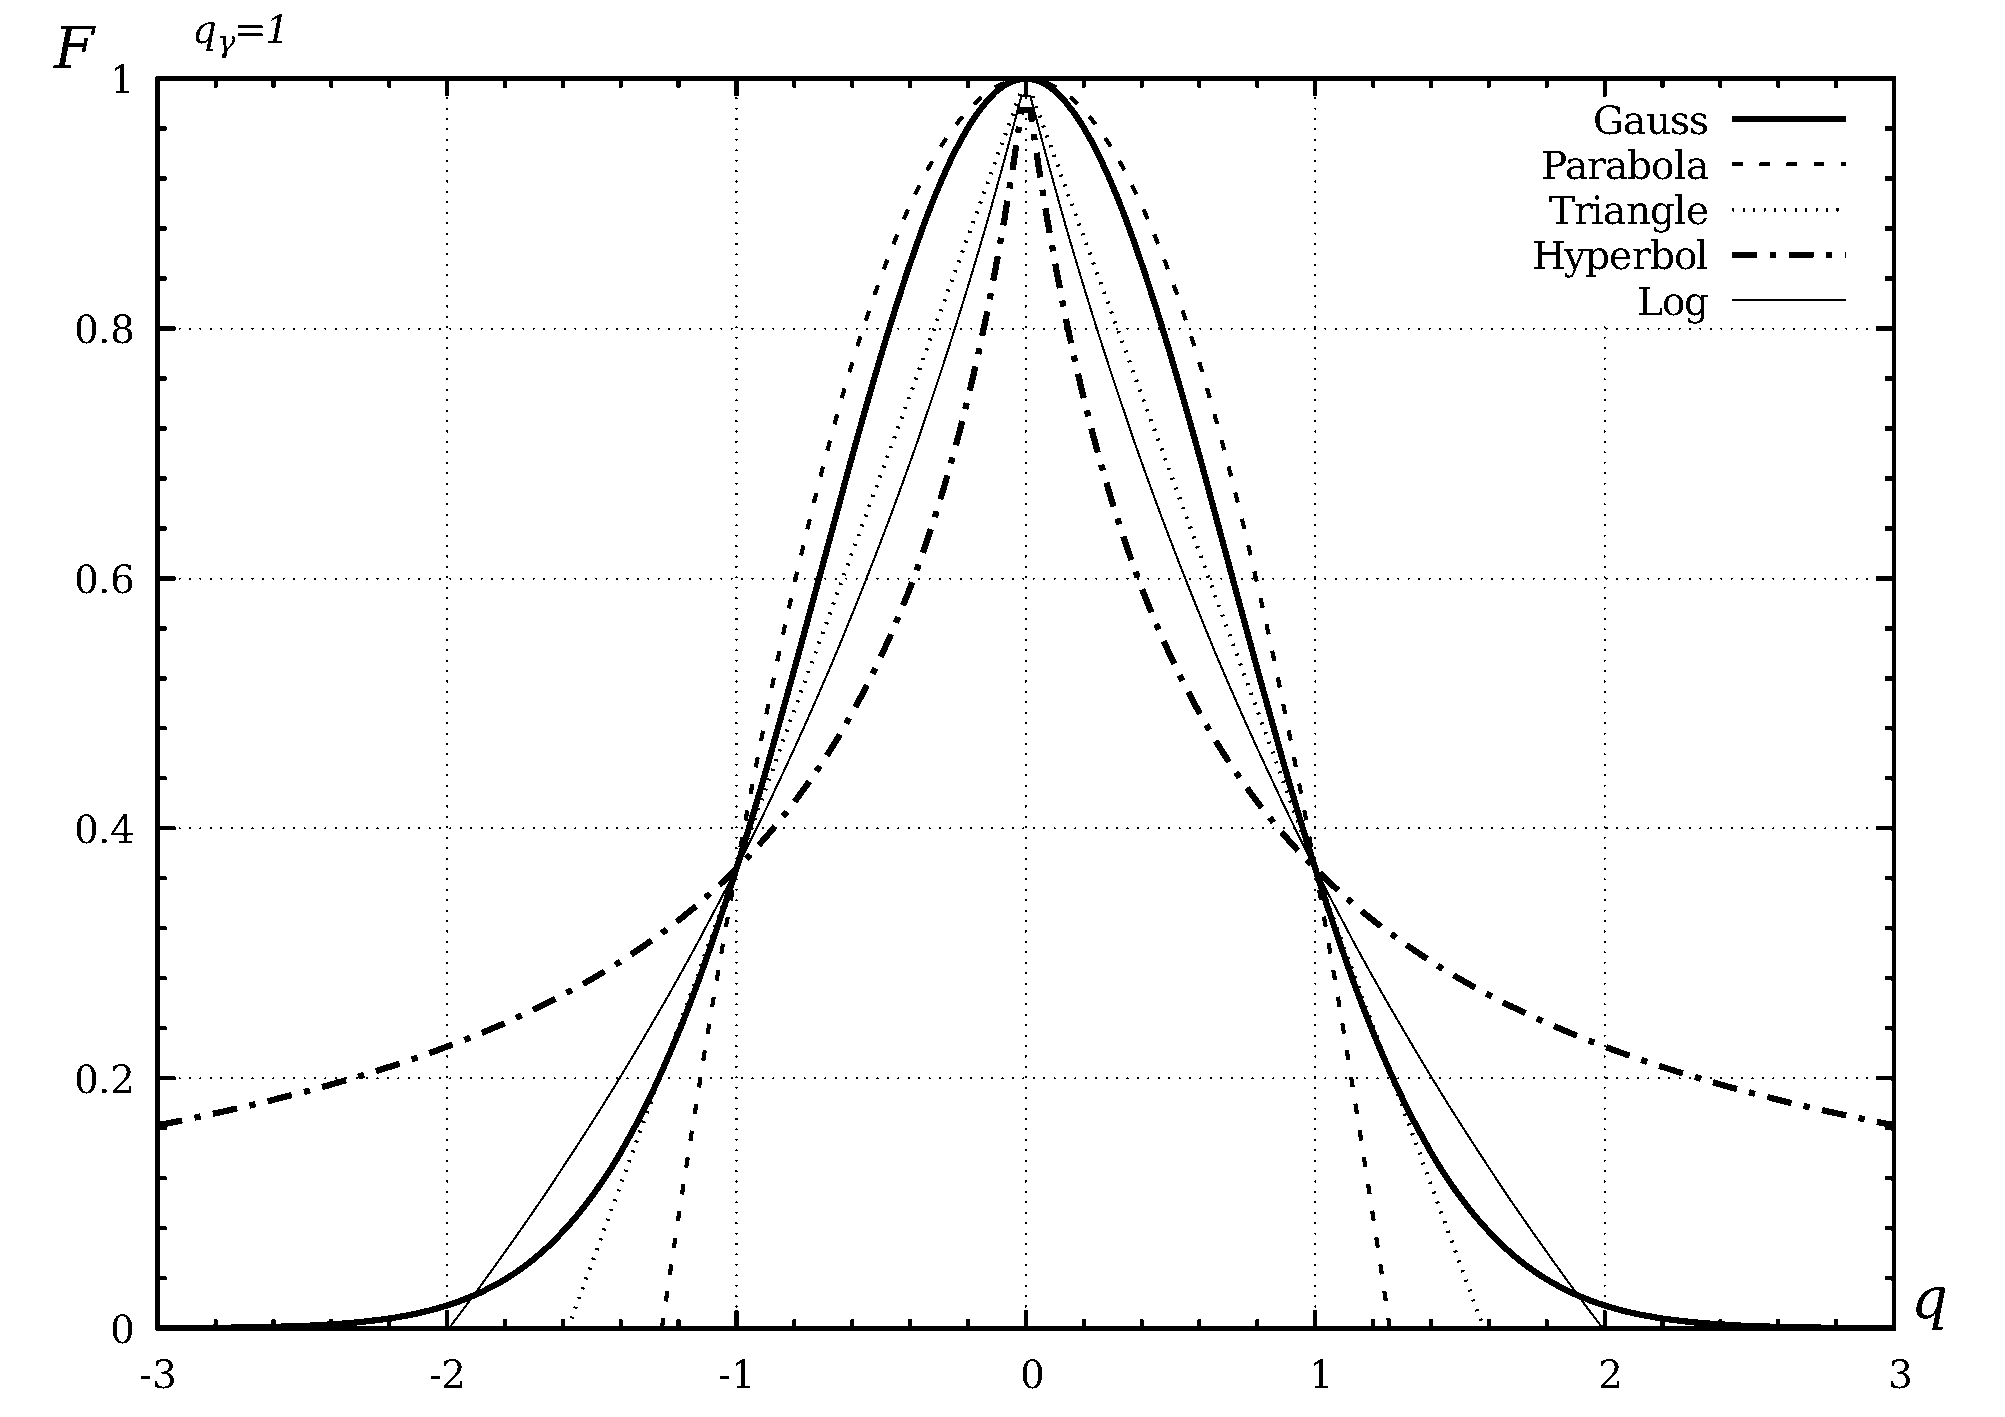
\includegraphics[width=45\TW]{p/F_types.png} }
  \caption{Функции качества идентификации (\ref{atu:eq:F_gauss})--(\ref{atu:eq:F_log})}
  \label{atu:f:F_types}
\end{figure}


% }}}2

% }}}1

\section{Структура поисковых систем}  % {{{1


Введемо необхідні для подальшого викладу визначення.

Визначення:
\textbf{пошуковий агент} --- це динамічна система, яка отримує вихідні ($x(t)$),
і, при необхідності, вхідні ($u(t)$) сигнали від однієї або кількох моделей,
величину оцінки стану об'єкта за критерієм ідентифікації,
може обмінюватися інформацією з іншими елементами пошукової системи,
та, на підставі значення критерію
ідентифікації, реалізує алгоритм настройки параметрів моделі (моделей) таким
чином, щоб забезпечити визначення заданого параметра.

Визначення:
\textbf{координатор пошуку} --- це динамічна система, яка отримує інформацію
від пошукових агентів і на підставі цієї інформації визначає
$p_{\mathrm{id}}(t)$ --- величину ідентифікованого параметра.
Крім цього, координатор може, на підставі цієї ж інформації,
керувати процесом адаптації всієї пошукової системи.


Таким чином, система ідентифікації складається з множини агентів, та
множини координаторів пошуку, які спільно вирішують задачу ідентифікації.
За винятком ієрархічних систем ідентифікації, найчастіше використовується один координатор пошуку.

У найпростішому випадку, коли використовується один пошуковий агент, обов'язки
агента і координатора можуть бути поєднані. Якщо відкинути цей вироджений
випадок, найбільш простою є ``плоска'' структура системи ідентифікації (рис.~\ref{atu:f:agents_flat}).
При цьому координатор отримує
інформацію від усіх пошукових агентів, і, при необхідності, управляє ними.


\begin{figure}[htb!]
\begin{center}
../../p3/p/agents.pgf
\end{center}
\label{atu:f:agents_flat}
\caption{Мультиагентна система ідентифікації з плоскою структурою}
\end{figure}

В более сложных случаях может использоваться иерархическая структура,
при этом каждый элемент, за исключением первого и последнего
уровня, служит как источником информации для последующего
уровня, так и координатором для предыдущего. При этом элемент
может как иметь непосредственно управляемую модель,
то есть выполнять роль агента, так и довольствоваться ролью промежуточного
координатора.

Деякі конфігурації агентів і координаторів в даний час практично
застосовуються, можливо під іншими позначеннями і для інших задач, деякі
введені вперше. Розглянемо деякі конфігурації.

\textbf{Рій} --- множина агентів, що забезпечує ідентифікацію за рахунок
концентрації максимальної кількості агентів в області передбачуваного максимуму
функції якості або ж заданого значення критерію. Три складові поведінки: рух
до оцінюваного локального екстремуму, до глобального, випадкова складова.

%\Cmt{define}

% \Cmt{Для сравнения требуется и это промоделировать.
% Достаточно накладно --- надо много агентов. Как вариант --- добавить вручную агентов вблизи
% экстремума.}

Достоинством данного подхода является простота алгоритмов,
которые должны быть реализованы агентами.
Недостатки --- требуется избыточное количество агентов.
Значительная часть агентов, находящихся вблизи экстремума,
практически не приносит информации. Роевые
алгоритмы (как и их прообразы в живой природе) ориентированы
для увеличения добычи ресурсов, а не информации. \Cmt{link}.
Также недостатком можно считать необходимость
получения информации от координатора (а именно, значение $p_\mathrm{id}$)
каждым агентом для возможности определения его динамики.

\textbf{Стрій} --- множина агентів, розташування яких, і якщо необхідно,
зміщення, задається однаковим чином. Відсутня індивідуальна динаміка кожного
агента. Нерухомий стрій утворює \textbf{сітку}.

как равномерно распределённую по пространству параметров,
так и нет.

Сложность алгоритмов, реализуемая каждым агентом в этом случае,
проще, чем в случае роя. Более того, передача информации от
координатора (в данном случае ``командира'') к агенту
является необязательной.
Тем не менее, возможности как адаптации,
так и просто повышения точности идентификации
у данного подхода сильно ограничены.

\textbf {Ансамбль} ---
множина агентів, що забезпечує ідентифікацію за рахунок розподілу агентів таким
чином, який забезпечує як точність ідентифікації за рахунок обмеженого
скупчення агентів в областях передбачуваних максимумів, так і оперативне
переключення на інші області при зміні параметрів за рахунок недопущення
невиправданої скупченості агентів~\cite{atu_ric2016}.

Возможно применение систем идентификации с структурами и поведением более высокого уровня,
но в данной работе они не рассматриваются.

У цієї роботі основна увага приділяється саме пошуковим структурам типу
``ансамбль ''. Очевидним недоліком даного підходу є відносна складність
алгоритмів, що реалізується пошуковими агентами.


% }}}1

\section{Свойства, параметры и алгоритмы работы поисковых агентов}  % {{{1 -----------

\subsection{Задачи, входные и выходные сигналы поисковых агентов} % {{{2 ------------

У відповідності до свого визначення, один пошуковий агент може керувати як
однією моделлю (рис.~\ref{atu:f:agent1}), \ref{atu:f:agent1q}),
так і кількома (рис.~\ref{atu:f:agent2}). При цьому він
може використовувати інформацію, як отриману безпосередньо від інших агентів,
так і обчислену в результаті обробки даних на інших рівнях системи
ідентифікації.

\begin{figure}[htb!]
\begin{center}
% vi:syntax=tex
\begin{tikzpicture}
  \bXStyleBloc{semiboldline,inner sep=2pt};
  \bXLineStyle{medline};
  % --- U
  \bXInput{U};
  % --- M
  \bXBlocL[2.0]{M}{$\mathbf{M}_i$}{U};
  \bXLink[$u(t)$]{U}{M};
  % --- Q
  \bXBloc[3.5]{Q}{$q(t)$}{M};
  \path (Q.east) ++(0.0,-1.0em) coordinate (Qqm);
  \path (Q.south west) ++(-0.3,-0.4) coordinate (BLKlb);
  \bXLink[$x_i(t)$]{M}{Q};
  % --- F
  \bXBloc[2.5]{F}{$F(q_o,q_{mi})$}{Q};
  \path (F.west) ++(0.0,-1.0em) coordinate (Fqm);
  \path (F.west) ++(0.0,+1.0em) coordinate (Fqo);
  \path (Fqo) ++(-1.6em,+2.8em) coordinate (Fqoi) {};  % external input
  \draw[medlinep] (Fqoi) |- (Fqo);
  \node[below right] at (Fqoi) {$q_o(t)$};
  \bXLink[$q_i(t)$]{Qqm}{Fqm};
  % --- P
  \bXBloc[2]{P}{$P$}{F};
  \draw[boldline,<->] (P.north) -- +(0,0.8);
  \path (P.north east) ++(0.1,+0.4) node (BLKrt) {};
  \bXLink[$F_i(t)$]{F}{P};
  % -- output
  \bXOutput[2.8]{Po}{P};
  \bXLink[$p_i(t)$]{P}{Po};
  \bXOutput[1.0]{Por}{P};
  \fill(Por) circle[radius=0.05];
  \bXLineStyle{semiboldline};
  \bXReturn{Por}{M}{$p_i(t)$};
  % -- block
  \draw[subelem] (BLKlb) |- (BLKrt) |- (BLKlb);
  \bXStyleBlocDefault;
  \bXDefaultLineStyle;
  %
  \TikzAddPadding
  %
\end{tikzpicture}

\end{center}
\caption{Пошуковий агент, який використовую функцію якості $F$, та управляє параметром однієї моделі}
\label{atu:f:agent1}
\end{figure}


\begin{figure}[htb!]
\begin{center}
% vi:syntax=tex
\begin{tikzpicture}
  \bXStyleBloc{semiboldline,inner sep=2pt};
  \bXLineStyle{medline};
  % --- U
  \bXInput{U};
  % --- M
  \bXBlocL[2.0]{M}{$\mathbf{M}_i$}{U};
  \bXLink[$u(t)$]{U}{M};
  % --- Q
  \bXBloc[3.5]{Q}{$q$}{M};
  \path (Q.east) ++(0.0,-1.0em) coordinate (Qqm);
  \path (Q.south west) ++(-0.3,-0.4) coordinate (BLKlb);
  \bXLink[$x_i(t)$]{M}{Q};
  % --- P
  \bXBloc[2]{P}{$P$}{Q};
  \draw[infoline,<->] (P.north) -- +(0,0.8);
  \path (P.west) ++(0.0,-1.0em) coordinate (Pqm);
  \path (P.west) ++(0.0,+1.0em) coordinate (Pqo);
  \path (Pqo) ++(-1.6em,+2.8em) coordinate (Pqoi) {};  % external input
  \path (P.north east) ++(0.1,+0.4) node (BLKrt) {};
  \bXLink[$q_{i}(t)$]{Qqm}{Pqm};
  \draw[medlinep] (Pqoi) |- (Pqo);
  \node[below right] at (Pqoi) {$q_o(t) \qquad A_i$};
  %\bXLink[$F_i(t)$]{F}{P};
  % -- output
  \bXOutput[2.8]{Po}{P};
  \bXLink[$p_i(t)$]{P}{Po};
  \bXOutput[1.0]{Por}{P};
  \fill(Por) circle[radius=0.05];
  \bXLineStyle{semiboldline};
  \bXReturn{Por}{M}{$p_i(t)$};
  % -- block
  \draw[subelem] (BLKlb) |- (BLKrt) |- (BLKlb);
  \bXStyleBlocDefault;
  \bXDefaultLineStyle;
  %
  \TikzAddPadding
  %
\end{tikzpicture}

\end{center}
\caption{Пошуковий агент, який використовую критерій $q$, та управляє параметром однієї моделі}
\label{atu:f:agent1q}
\end{figure}


\begin{figure}[htb!]
\begin{center}
% vi:syntax=tex
\begin{tikzpicture}
  %\draw[hair,step=1.0em] (0,-3) grid (12.0,3.0);
  \bXStyleBloc{semiboldline,inner sep=2pt};
  \bXLineStyle{medline};
  % --- U
  \bXInput{U};
  \path (U.center) ++(2.5em,0.0em) coordinate (UxM);
  \draw (U.center) -- (UxM);
  \fill (UxM) circle[radius=0.05];
  \node[above right] at(U) {$u(t)$};
  % --- M0
  \bXBranchy[2]{UxM}{U0};
  %\fill[red](U0) circle[radius=0.05];
  \bXBlocL[2.0]{M0}{$\mathbf{M}_{i0}$}{U0};
  \bXLinkyx{UxM}{M0};
  % --- M1
  \bXBranchy[-2]{UxM}{U1};
  %\fill[green](U1) circle[radius=0.05];
  \bXBlocL[2.0]{M1}{$\mathbf{M}_{i1}$}{U1};
  \bXLinkyx{UxM}{M1};
  % --- A
  \path (M0.east) ++(3.1em,0.0em) coordinate (X0);
  \path (X0) ++(4.0em,0.0em) coordinate (P0S);
  \path (X0) ++(0.0em,-2.0em) coordinate (Alb);
  %\fill[red](Alb) circle[radius=0.05];
  \path (M1.east) ++(3.1em,0.0em) coordinate (X1);
  \path (X1) ++(4.0em,0.0em) coordinate (P1S);
  \path (X1) ++(0.0em,2.0em) coordinate (Alt);
  \path ( $0.5*(P0S) + 0.5*(P1S)$ ) coordinate(PS);
  \path ( $0.5*(X0) + 0.5*(X1)$ ) coordinate(QO);
  \draw[medlinep] (QO) ++(-3.2em,0em) -- (QO);
  \node[above left] at(QO) {$q_{o}(t)$};
  %\fill[green](Alt) circle[radius=0.05];
  \draw[boldline] (Alb) -- ++(4.0em,0.0em) |- (Alt) -- cycle; % ----- MAIN block
  \draw[medlinep] (M0.east) -- (X0); // % inputs: x_ix(t)
  \node[above right] at(M0.east) {$x_{i0}(t)$};
  \draw[medlinep] (M1.east) -- (X1);
  \node[above right] at(M1.east) {$x_{i1}(t)$};
  \draw[semiboldlinep] (P0S) -- ++(3.0em,0em) -- ++(0em,-3.0em) -| (M0.south); % -- out params
  \node[above right] at(P0S) {$p_{i0}(t)$};
  \draw[semiboldlinep] (P1S) -- ++(3.0em,0em) -- ++(0em,+3.0em) -| (M1.north);
  \node[above right] at(P1S) {$p_{i1}(t)$};
  \draw[medlinep] (PS) -- ++(4.0em,0em);
  \node[above right] at(PS) {$p_{i}(t)$};
  \path (PS) ++(-2.1em,0.0em) coordinate (AI);
  \node at(AI) {$\mathbf{A}_{i}$};
  %
  \TikzAddPadding
  %
\end{tikzpicture}

\end{center}
\caption{Пошуковий агент, який управляє параметрами двох моделей}
\label{atu:f:agent2}
\end{figure}

Для спрощення позначень величин, що належать різним агентам, ведемо
позначення. Якщо в даному контексті важливо вказувати індекс агента, то він
вказується явно, наприклад: $F_{c, i} (t)$ --- значення функції якості для
центральної (``c'') моделі агента з індексом ``i''. У тих випадках, коли
обрано конкретний агент або коли позначення застосовується до всієї множині
агентів, індекс можна вилучити, наприклад: $ p_e (t)$
--- оцінка значення параметра для поточного агента або ж для агентів взагалі.
Для позначення найближчого околу агента використовуємо такі позначення:
``c'' --- ``center'' --- позначає центральну або єдину модель агента або ж
відноситься до агенту в цілому, ``l'' --- ``left'' --- позначає, в
залежності від контексту, або величину, яка відноситься до попереднього (за
індексом) агенту, або ж першу модель (з двох або трьох), яка використовується
агентом, ``r'' --- ``right'' --- аналогічно, але в протилежну сторону у
просторі індексів.
Якщо ж необхідно вказати індекс агента, а величина щодо
об'єкта має позначення ``c'', то цю частину позначення можна опустити,
наприклад: $p_i (t) \equiv p_{i, c} (t)$, $q_{i , c} \equiv q_{i} (t)$.
Всі індекси одночасно опускати не можна, однак, в очевидних випадках можна
опускати явну залежність від часу: $q_l (t) \equiv q_l$. При необхідності,
що величина відноситься до моделі, без вказівки конкретного індексу моделі,
будемо використовувати індекс ``m'', наприклад $x_m$ --- вихідний сигнал
заданої (або ж єдиною) моделі.

В случае, когда один агент настраивает несколько моделей,
или/и, если пространство параметров имеет размерность больше единицы,
вместо простого индекса $i$ могут применяется составные.

Кожен агент на підставі як власних вимірів, так і інформації, отриманої від
інших агентів, оцінює значення $p_e (t)$, яке, за його даними, найближче до
параметра об'єкту $p_o(t)$.
Частина методів використовує це подання неявним чином. При цьому,
якщо значення $p_e$ виходить за межі значень параметрів моделей, на підставі
яких було отримано це значення, то його слід вважати сумнівним.
Ступінь ``впевненості'' в розрахунковому значенні $p_e$ позначимо $S \in [0; 1] $\label{atu:d:S} (surety).
В результаті такі оцінки в подальшому можна як
взагалі не враховувати при розгляді, так і обмежити їх вплив на наступному
рівні.
Або --- можна обмежити область допустимих значень $p_e$
значеннями параметрів моделей, що використовуються.

Выходными сигналами агента являются:\label{atu:d:agent_out_list}

\begin{itemize}

  \item
    $p_c(t)$ --
    текущее значение параметра.

  \item
    $p_e(t)$\label{atu:d:p_e} --
    текущее значение оценки параметра.

  \item
    $F_c(t)$ ---
    текущее значение функции качества
    (если используется одна  модель для агента, или же если агент каким-либо образом её усредняет
    или аппроксимирует в случае нескольких моделей).
    Может совмещать функции входного и выходного сигналов.

  \item
    $q_c(t)$ ---
    значение критерия качества (аналогично предыдущей величине в случае нескольких моделей);
    изначально этот сигнал был представлен как входной для агента, тем не менее
    он может использоваться и на более высоких уровнях системы идентификации.
    Если же агенту значение критерия недоступно, то и в списке выходных сигналов эта величина
    также отсутствует.

  \item
    $F_e(t)$ ---
    аппроксимированное значение функции качества
    в точке $p_e(t)$. Если агент не использует для работы аппроксимацию
    $F$, то и выходного сигнала нет.

  \item
    $S(t)$ ---
    степень ``уверенности'' агента в полученном значении.

\end{itemize}

Некоторые из этих сигналов могут не использоваться в конкретной реализации
координатора поиска. Например, системы идентификации с одним агентом
практически не нуждаются в величине $S(t)$. Величина $q_c(t)$
достаточно редко используется при работе координатора.
Достаточно часто используются производные сигналы,
например $W(t) = F_c(t) S(t)$ (worthiness), совмещающий как локальную
уверенность агента в оценке $p_\mathrm{id}(t)$,
так и глобальную функцию качества.
Также указанные сигналы могут использоваться самим агентом непосредственно,
для определения собственной динамики.


Агенти, для оцінювання величини $p_e$ можуть використовувати як значення
критеріїв ідентифікації $q$ безпосередньо, так і тільки значення функцій
якості, які відповідають критеріям.

Принципиальной разницы между конфигурациями
``один агент --- пара моделей''
и
``два агента, каждый управляет одной моделью'' нет.
Для определённости будем считать, что если поддерживается
постоянная разность между значениями параметров моделей,
или же эта разность определяется единообразно,
то это --- один агент. Если же разность
не определяется напрямую, и является следствием динамики каждой модели,
то имеет смысл говорить о паре агентов.

Тем не менее, при использовании пары моделей неоправданно много времени
тратится на перемещение поисковой пары, особенно при резких изменениях
идентифицируемого параметра. Поэтому, использование множества
поисковых агентов может кардинально уменьшить время идентификации.


Рассмотрим случай, когда каждый агент взаимодействует с двумя своими ближайшими соседями.
Для того, что бы обработать границы поисковой области есть несколько подходов,
которые требуют определения дополнительных моделей, использование которых
и обеспечивает как ограничение области поиска, так и единообразность
алгоритмов для агентов внутри.
В дальнейшем будем обозначать их индексами ``ll'' и ``rr''.

Для систем идентификации, использующих только один агент с двумя моделями,
это достаточно неплохой вариант.
Если же использовать несколько агентов, каждый с парой моделей,
то модели в этой системе будут использоваться нерационально.
Рассмотрим случай, когда значения параметров моделей распределены в пространстве
параметров последовательно, и значение параметра, соответствующее $q_o$ лежит между значениями
параметров пары соседних моделей.
При этом, если пара моделей принадлежит одному агенту, то он,
а следовательно, и вся система идентификации может достаточно точно
оценить значение $q_o$. Если же модели этой пары
принадлежат разным агентам --- то нет.

Для того, что бы нивелировать этот недостаток,
попробуем создать систему идентификации,
в которой количество моделей равно количеству агентов,
не считая, может быть, дополнительных моделей на границе рабочей области.

% TODO: really define!!!!!!!!!!!!!


Первый из подходов реализуется наиболее простым способом
и практически не требует затрат.
В этом случае для единообразия множество моделей дополняется двумя
(в одномерном случае) неподвижными псевдомоделями (fake models).
Для псевдомоделей считаем $  F_{ll} = F_{rr} = 0$,
а координаты выбираются за пределами рабочего диапазона поиска.
Применение этого подхода наиболее оправданно для агентов,
вычисляющих значение $p_e$ с помощью функции качества.
При этом, платой за меньшие вычислительные затраты
является появление ``сжимающего'' воздействия на весь ансамбль в целом.
Системы с агентами, которые используют для определения $p_e$ непосредственно значение критерия,
не могут напрямую воспользоваться этом подходом,
так как нулевому (или близкому к нулевому) значению функции качества
обычно соответствует неограниченное множество значений критерия.

Второй подход отличается применением неподвижных настоящих моделей
на границе рабочей области. При этом, агенты, соседствующие с этими моделями,
могут использовать  значения как параметров, так и критериев этих
моделей естественным образом. Основным недостатком этого подхода
является дополнительный расход ресурсов для моделей на границе.
Также применение таких моделей может быть затруднительно тех случаях,
когда моделирование за пределами (или непосредственно на границе)
невозможно из-за нарушения устойчивости моделей.
Тем не менее, этот подход, с одной стороны,
позволяет корректно применять агентов, использующих $q$,
а с другой --- позволяет избавиться от ``сжимающего'' воздействия
при использовании агентов, использующих $F$.

Промежуточным вариантом является подход,
при использовании которого тоже используются
псевдомодели, но вместо нулевого значения
функции качества используется или каким-либо образом аппроксимированное
значение $F$, (применимо и к $q$), или полученное в результате
предварительного моделирования.


% }}}2



\subsection{ Методы определения искомого значения параметра одним агентом }  % {{{2

Першою із задач, що постають перед агентом ідентифікації, є визначення $p_e(t)$
на підставі наявних даних, а також оцінка впевненості $S(t)$ в
отриманому значенні.

Системы поисковой и адаптивно-поисковой идентификации,
используемые для работы с обычными нелинейными динамическими системами,
в качестве исходных данных как для определения непосредственно
искомого параметра, так и для построения поисковой траектории
использовали непосредственно выходные сигналы объекта ($x_o(t)$) и модели~($x_m(t)$).
При этом явно или неявно использовалась функция качества.
Более того, при определённых условиях, с учётом
инерционных и усредняющих свойств системы идентификации
такой подход, неявным образом, использовал
один из энергетических критериев.

При идентификации систем хаотической динамики
использование критерия идентификации является обязательным.
Естественно, это применимо и для систем, не проявляющих
хаотическую динамику. При этом агент,
для выполнения своих задач, может использовать
как как само значение критерия, так и соответствующее ему
значение функции качества. Алгоритмы,
используемые агентами в этих случаях,
будут существенно отличаться. В первую очередь
это связано с тем, что чётный вид функций качества
побуждает использовать для определения максимума
методы, характерный для систем экстремального управления.

Для непротиворечивости и сохранения работоспособности системы идентификации в широких
пределах имеет смысл рассмотреть набор необязательных,
но желательных требований:

\begin{itemize}

  \item
    В первую очередь, при линейной зависимости $q(p)$ и отсутствии ошибок измерения
    ошибка оценивания ``своей'' точки $p_e$ должна быть достаточно малой.
    Нарушение этого требования затрудняет работу системы идентификации
    при приближении к идентифицируемому значению.

  \item
    Во-вторых,
    при этих же условиях глобальные оценки $p_o$ также должны также
    характеризоваться достаточно малыми ошибками, в противном случае
    теряется смысл использования нескольких агентов.

  \item
    Сближение и удаление поисковых агентов в пределах назначенных
    диапазонов не должно приводить к существенному изменению величины
    идентифицируемого значения. Это требование по большей части выполнимо
    только на достаточно ``хороших'' видах критериев, без
    преобладающего влияния высокочастотных нелинейных эффектов,
    однако сам метод не должен вносить существенные дополнительные
    искажения на данном этапе.

\end{itemize}

Следует также отметить, что для реальных задач
$q_o(p) \ne q_m(p)$ ввиду как ограниченности моделей,
так и помех измерения. Тем не менее,
в данной главе данный факт будет игнорироваться
с целью изучения возможностей и ошибок
собственно методов идентификации.




Как уже было отмечено, в задачи агента входит
не только определение величины $p_e$,
но и оценка собственной ``уверенности'' $S$
в полученном значении. Рассмотри факторы,
которые может учитывать агент при решении этой задачи.

\begin{enumerate}

  \item Относительная удалённость точки $p_e$ от точек, использовавшихся при
    её определении. При этом может приниматься во внимание или только центральная точка $p_c$,
    или же учитываться точки соседних агентов.

  \item
    Расположение $p_e$ относительно используемых агентов. Как правило, ошибки при интерполяции
    заметно меньше ошибок при экстраполяции, и это необходимо учитывать. Также,
    сама конфигурация используемых точек может быть более или менее благоприятна
    для оценки~$p_e$.

  \item
    В при использовании некоторых методов есть возможность оценить нелинейность
    зависимости $q(p)$, и следовательно, учесть это при определении $S$,
    с помощью коэффициента~$k_l$.

  \item
    При оценке могут возникать особые случаи, препятствующие
    нормальной работе метода. Следовательно, такие случаи требуют применения особых правил
    при вычислении~$S$.

\end{enumerate}

Пропонуються наступні
методи визначення $S$ при отриманні агентом інформації з трьох моделей:
%
\begin{equation}
  S_1 = c_\mathrm{su} \exp \left( - \frac{ \big( k_l c_\mathrm{dist} ( p_e - p_c ) \big)^2 }{p_b^2} \right)
  ,
  \label{atu:eq:S1}
\end{equation}
%
\begin{equation}
  S_3 = c_\mathrm{su} \exp \left( - \frac{ \big( k_l c_\mathrm{dist} \min( |p_e - p_l|,|p_e - p_c|, |p_e - p_r| ) \big)^2 }{p_b^2} \right)
  .
  \label{atu:eq:S3}
\end{equation}
%
де
$c_\mathrm{su}$ ---
коефіцієнт, що відображає працездатність методу в даному випадку;
$c_\mathrm{dist}$ ---
коефіцієнт, що визначає ``штраф'' або ``бонус'', пов'язаний з відносним розташуванням робочих точок;
$k_l$ ---
коефіцієнт оцінки нелінійності системи;
$p_b$ ---
характерний масштаб, щодо якого враховується видалення $p_e$ від використаних точок.


У випадках, коли агенти рівноправні, має сенс використовувати визначення
(\ref{atu:eq:S3}), так як похибка визначення $p_e$ в першу чергу визначається її
віддаленістю від найближчого агента. В даній роботі, якщо не вказано інше, буде
використовуватися саме воно.
%
Использовать определение (\ref{atu:eq:S1}) имеет смысл в тех случаях,
когда информация, полученная от соседних агентов, менее надёжна, чем от текущего,
например, при использовании псевдомоделей.

\paragraph{Демонстрационная задача}

Для демонстрації способів визначення пошуковим агентом величини $p_e$ в
стаціонарному або квазістаціонарному випадку введемо наступну штучну залежність~$q(p)$:
%
\begin{equation}
  q_\mathrm{dem}(p) = q_{00} + c_\mathrm{lin} \tilde{p} + c_\mathrm{s1} \sin( \pi \tilde{p} ) + c_\mathrm{s2} \sin( 2 \pi \tilde{p} ) + c_\mathrm{s20} \sin( 20 \pi \tilde{p} ),
  \label{atu:eq:q_dem}
\end{equation}
%
де
$q_{00}$, $c_\mathrm{lin}$, $c_\mathrm{s1}$, $c_\mathrm{s2}$, $c_\mathrm{s20}$
--- коефіцієнти, що дозволяють налаштувати цю залежність для перевірки заданого аспекту поведінки агента,
$ \tilde{p} = \frac{p - p_{\min}}{p_{\max} - p_{\min}} $ ---
параметр, приведений до безрозмірного вигляду.
При цьому
$\tilde{p} \in[0;1]$, $c_\mathrm{lin} \ne 0$
визначає лінійну частину залежності,
$c_\mathrm{s1}$ і $c_\mathrm{s2}$
визначають нелінійну частину, що має характерний масштаб порядку робочого діапазону $p$,
$c_\mathrm{s20}$
визначає високочастотну складову цієї залежності.
Якщо $c_\mathrm{s1} = 0$, $c_\mathrm{s2}=0$, $c_\mathrm{s20}=0$,
то задача визначення $p_e$ є тривіальною,
але такий випадок також є корисним при аналізі поведінки агента.

В дальнейшем будем использовать эти обозначения при описании
различных режимов работы методов идентификации, а также
при моделировании тестовых задач.

Рассмотрим возможные способы определения $p_e$ для агентов,
использующих как критерий идентификации непосредственно,
так и функции качества.

% }}}2


\subsection{Методы агентов, использующих значения критерия }  % {{{2

Нерухомий агент, який використовує для своєї роботи тільки одну модель, і,
відповідно, характерне для неї значення критерію, практично не має самостійного
сенсу.
%
Реальная польза от такого агента
может быть только в том случае, когда координатор
каким-то образом смог оценить зависимость $q(p)$ целиком,
и передал или эту зависимость агенту, или по его запросу вычисляет $p(q)$.
Очевидно, что в таком случае никакие поисковые агенты не нужны,
и можно просто вычислить $p(q_o)$.

Если агент, использующий одну модель является подвижным,
то он может оценить своё положение, используя историю.
Представление истории может иметь различные формы.
Например, агент может хранить значения $p_c$, $q_c$
для момента времени в прошлом, отстоящем от текущего
на заданное значение. Может быть применён какой-либо
сглаживающий фильтр, в котором влияние различных моментов прошлого учитывается
с различными коэффициентами. Также в качестве функции
представления истории может использоваться
динамика самого идентифицируемого объекта~\cite{mich_92}.

Рассмотрим случай, когда один подвижный агент и получает данные с двух моделей,
$ \mathbf{M}_{il}$ и
$ \mathbf{M}_{ir}$,
и управляет ими единообразным образом, например
выдерживая постоянное расстояние $\Delta p$ между ними в пространстве параметров.
В этом случае он может оценить, какая из моделей ближе по критерию
к объекту, и оценить положение $p_o$ как $p_e$.

Розглянемо групу з трьох агентів:
$\mathrm{A}_l$,
$\mathrm{A}_c$,
$\mathrm{A}_r$.
Агент $\mathrm {A} _c$ зі значенням параметра $p_c$ сам визначає величину
$q_c$, від сусідніх агентів отримує значення $p_l$, $q_l$, $p_r$, $q_r$.
Будемо вважати, що динаміка агентів визначена так, що
$p_l(t) < p_c (t) < p_r(t) \; \forall t$.
Система ідентифікації забезпечує кожного агента
значенням $q_o$.
Зважаючи на все вищезазначене,
задача
визначення $p_e$ полягає в знаходженні такого $p$, яке відповідає перетину
невідомою кривої, заданої трьома точками, з прямою $q = q_o$.
Формально, з урахуванням введених обмежень, три точки однозначно визначають параболу. Однак,
застосування параболічної апроксимації в умовах високого рівня перешкод
найчастіше невиправдано~\cite{atu_asau27}.
Більш того, в цьому випадку буде потрібна додаткова
логіка як для вибору підходящого кореня, так і для визначення ``впевненості''
в отриманому рішенні.
Тому, будемо розглядати кусково-лінійне наближення з
аналізом отриманої конфігурації. Існує чотири можливих конфігурації,
кожна з яких потребує окремого рішення.

Рассмотри возможные конфигурации в порядке,
обеспечивающем непротиворечивость алгоритма.

\paragraph{Случай 1.}
Это особый случай, когда значение $p_c$ агента
достаточно хорошо совпадает с искомым значением.
Понятие ``достаточно хорошо'' в данном случае определяется
поставкой задачи, и может быть задана предельным значением
функции качества: $F_c > F_{\mathrm{good}}$, где $F_{\mathrm{good}}$
выбирается достаточно близко к единице.
При этом считаем:
%
\[
p_e = p_c, \; c_\mathrm{su} = 1, \;  c_\mathrm{dist} = 1, \;  k_l = 1, \;  p_b = p_r - p_l,
\]
%
что даёт $S = 1$, т.е. агент полностью ``уверен''
в полученном значении $p_e$. Если есть явное ограничение
на использование функции качества непосредственно агентом,
то следует задать допуск на значение критерия:
$ |q_c-q_o| < q_{\min}$.

Практически, для нескольких агентов может одновременно
может выполнится данное условие, и
дальнейшее определение $p_\mathrm{id}$ в этом противоречивом случае
возлагается на координатора поиска. Если данная
ситуация в процессе поиска случается достаточно редко,
то это, как правило, не нарушает общую динамику поиска.
Если же этот случай проявляется достаточно часто,
то это свидетельствует о грубых просчётах
при синтезе системы идентификации.
Например, такое поведение может вызвать применение
критерия, неподходящего для данной задачи,
или же предельно заниженная чувствительность функции качества.

Следует отметить, что в этом случае у агента нет необходимости
анализировать значения, полученные от соседних агентов.
Это позволяет избежать ряда ситуаций, в которых
алгоритм поиска будет давать сбои, связанные неопределённостью
алгоритмов поиска в вырожденных случаях.
%
В першу чергу, якщо
$F_c \le F_\mathrm{good}$, то $q_o -q_c \ne 0$,
і можна застосувати наступні перетворення:
%
\[
  \tilde{p}_l = p_l - p_c;
  \quad
  \tilde{p}_c = p_c - p_c = 0;
  \quad
  \tilde{p}_r = p_r - p_c;
  \quad
  \tilde{p}_e = p_e - p_c;
\]
\begin{equation}
  \tilde{q}_l = \frac{q_l-q_c}{q_c-q_o};
  \quad
  \tilde{q}_c = \frac{q_c-q_o}{q_c-q_o} = 1;
  \quad
  \tilde{q}_l = \frac{q_l-q_c}{q_c-q_o}.
  \label{atu:eq:q_agent_rel}
\end{equation}
%
При цьому критерій приводиться до безрозмірного вигляду, причому точку відліку і одиничну довжину визначають величини
$q_c$ и $q_o$, так як $\tilde{q_c} = 1$ і $\tilde{q_o} = 0$.
У просторі параметрів відбувається тільки зміщення точки відліку.

Зважаючи на ці позначення визначимо оцінку
$\tilde{p}_e$
для кожної з ділянок незалежно:
%
\begin{equation}
  \tilde{p}_{el} = \frac{\tilde{p}_l}{1-\tilde{q}_l},
  \quad
  \tilde{p}_{er} = \frac{\tilde{p}_r}{1-\tilde{q}_r}.
  \label{atu:eq:pr_ex}
\end{equation}

Випадок точної рівності нулю знаменника в цих виразах відповідає нескінченно
далекому розташуванню $p_e$, повної непевності в отриманому рішенні ($S = 0$)
і алгоритмічно виключається.


\paragraph{Случай 2.} % brIdx = 3,4,5,6
Все значения $q_l$, $q_c$, $q_r$ лежат по одну сторону
сторону от прямой $q=q_o$,
что эквивалентно условию $\tilde{q}_l > 0  $ и $\tilde{q}_r > 0  $.
В этом случае следует принять,
что $p_e \notin [p_l, p_r]$, то есть по данным текущих трёх моделей
нет возможности достаточно уверенно определить $p_e$. Тем не менее,
задача оценить $p_e$ всё равно остаётся актуальной.
Если система идентификации использует только одного агента,
то значение $p_e$, пусть даже ненадёжное, необходимо для
определения динамики агента, и соответственно, смещении
его в сторону области, где оценка будет более обоснованной.
Если же используется мультиагентная система,
то полученное значение $p_e$ достаточно или ограничить искусственно,
или уменьшить его значимость за счёт снижения величины $c_\mathrm{su}$.

При анализе данного случая необходимо рассмотреть несколько
вариантов.

Вариант A.\label{atu:d:p_eql_2A} % brIdx = 3
Центральная точка --- наилучшая~(рис.~\ref{atu:f:pq_2A}),
т.е $\tilde{q}_l > 1 $ и $\tilde{q}_r > 1  $.

\begin{figure}[htb!]
  \centerline{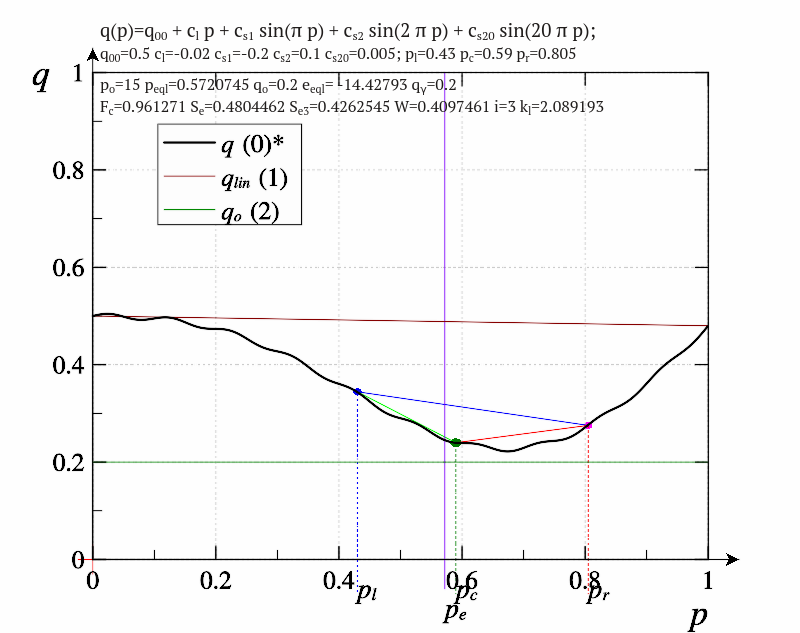
\includegraphics[width=60\TW]{p/pq_sin-p_pq_cgood.png} }
  \caption{Конфигурация точек, соответствующая случаю 2A}
  \label{atu:f:pq_2A}
\end{figure}

Как видно из графика, это достаточно нетривиальная конфигурация,
которая может соответствовать локальному приближению
$q(p)$ к $p_o$, что для хорошего критерия нехарактерно,
временной конфигурации рабочих точек из-за влияния помех,
а также возможности реального нахождения $p_o$
в текущем рабочем диапазоне, но из-за определённых причин,
прежде всего сильной нелинейности $p(q)$
неправильной оценке его положения.
На основании имеющейся информации сложно сделать вывод
о реальных причинах, поэтому
в этом случае производится минимальная корректировка положения,
и уверенность в полученном решении невелика:
%
\begin{equation}
  \tilde{p}_e = 0.1 ( \tilde{p}_{el} + \tilde{p}_{er} ),
  \;
  c_\mathrm{su} = 0.2, \;  c_\mathrm{dist} = 4, \;   p_b = p_r - p_l,
  \label{atu:eq:pr_e_2A}
\end{equation}



Вариант B.\label{atu:d:p_eql_2B} % brIdx = 4,5
Центральная точка --- промежуточная~(рис.~\ref{atu:f:pq_2B}).
Соответствует условию
$ ( \tilde{q}_l -1 ) \cdot ( \tilde{q}_r -1 ) < 0 $.

\begin{figure}[htb!]
  \centerline{
    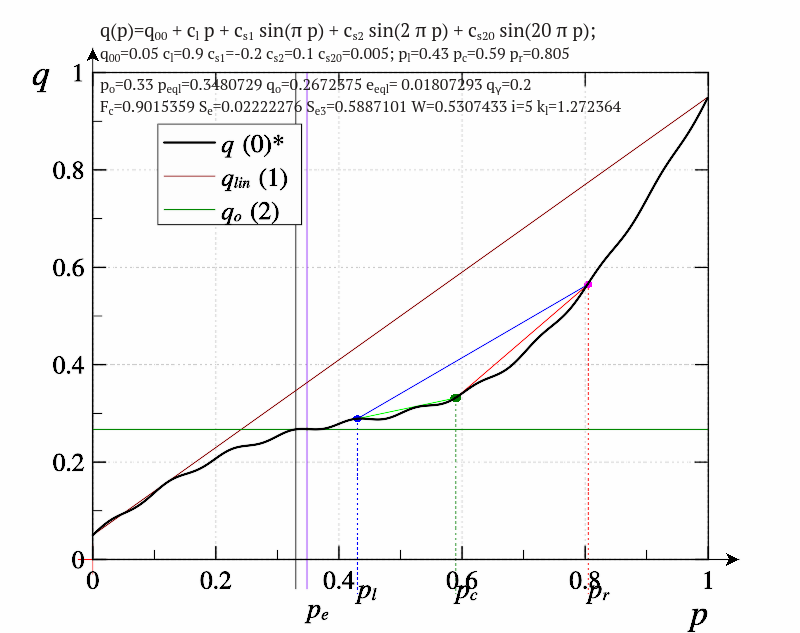
\includegraphics[width=49\TW]{p/pq_sin-p_pq_po=033.png}
    \hfill
    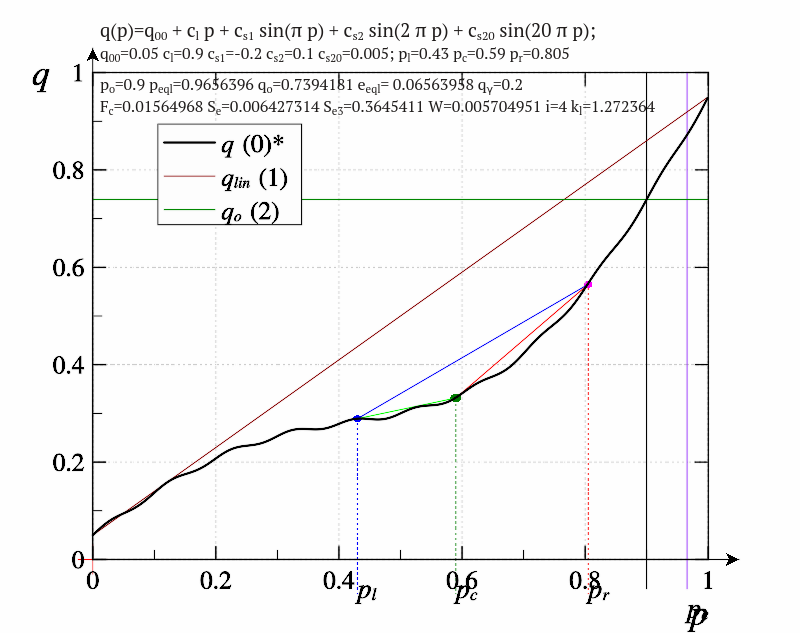
\includegraphics[width=49\TW]{p/pq_sin-p_pq_po=090.png}
  }
  \caption{Конфигурации точек, соответствующие случаю 2B}
  \label{atu:f:pq_2B}
\end{figure}

Эта конфигурация не является неопределённой, как в предыдущем случае,
и соответствует экстраполяции зависимости за пределы $[p_l, p_r]$.
В этом случае будем использовать
%
\begin{equation}
  \tilde{p}_e
  =
  \begin{cases}
    \tilde{p}_{el}, & \tilde{q}_l < \tilde{q}_r
    \\
    \tilde{p}_{er}, & \text{ otherwise}.
  \end{cases}
  ,
  c_\mathrm{su} = 0.9, \;  c_\mathrm{dist} = 2,  \;
  p_b =
  \begin{cases}
    -\tilde{p}_l, & \tilde{q}_l < \tilde{q}_r
    \\
    \tilde{p}_r, & \text{ otherwise}.
  \end{cases}.
  \label{atu:eq:pr_e2B}
\end{equation}

Относительно высокое значение
$ c_\mathrm{su}$ и достаточно ограниченное значение $c_\mathrm{dist}$
подчёркивают тот факт, что несмотря на наличие экстраполяции,
метод в этом случае может давать неплохие результаты.


Вариант C. \label{atu:d:p_eql_2C}% brIdx = 6
Центральная точка --- наихудшая~(рис.~\ref{atu:f:pq_2C}).

\begin{figure}[htb!]
  \centerline{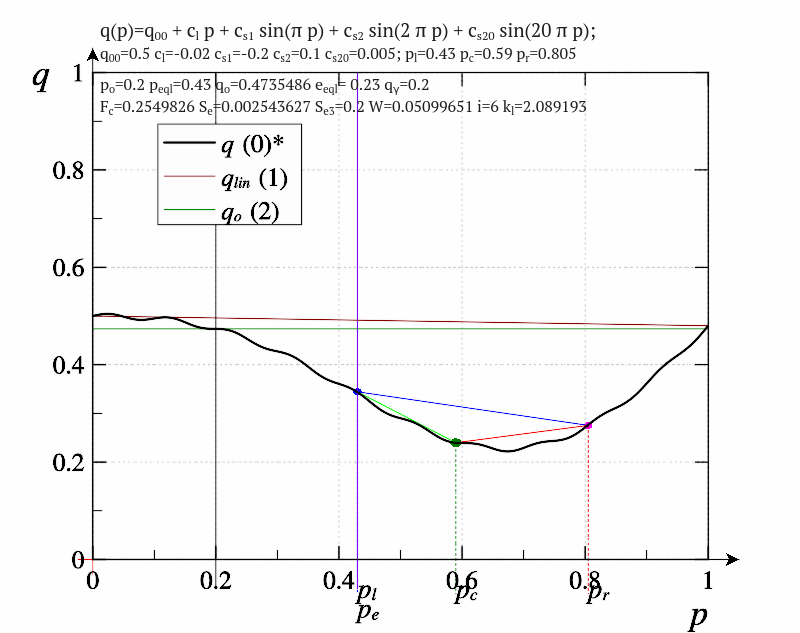
\includegraphics[width=60\TW]{p/pq_sin-p_pq_cbad.png} }
  \caption{Конфигурация точек, соответствующая случаю 2C}
  \label{atu:f:pq_2C}
\end{figure}

Этот вариант один из наименее благоприятных для определения $p_e$,
ещё более неопределённый по сравнению со случаем 2A.
В этом случае в качестве $p_e$ можно взять лучшую из крайних точек,
при этом нулевое расстояние от этой точки в определении $S$
необходимо скомпенсировать существенным штрафом в значении $c_\mathrm{su}$,
остальные коэффициенты при этом значения не имеют:
%
\begin{equation}
  \tilde{p}_e
  =
  \begin{cases}
    \tilde{p}_{l}, & \tilde{q}_l < \tilde{q}_r
    \\
    \tilde{p}_{r}, & \text{ otherwise}.
  \end{cases}
  ,
  c_\mathrm{su} = 0.1 .
  \label{atu:eq:pr_e2C}
\end{equation}

\paragraph{Случай 3.} % brIdx = 10
Значения $q_l$ и $q_r$ лежат по одну сторону от прямой $q=q_o$,
а $q_c$ --- по другую, то есть существуют два корня в рассматриваемой области~(рис.~\ref{atu:f:pq_3}).

\begin{figure}[htb!]
  \centerline{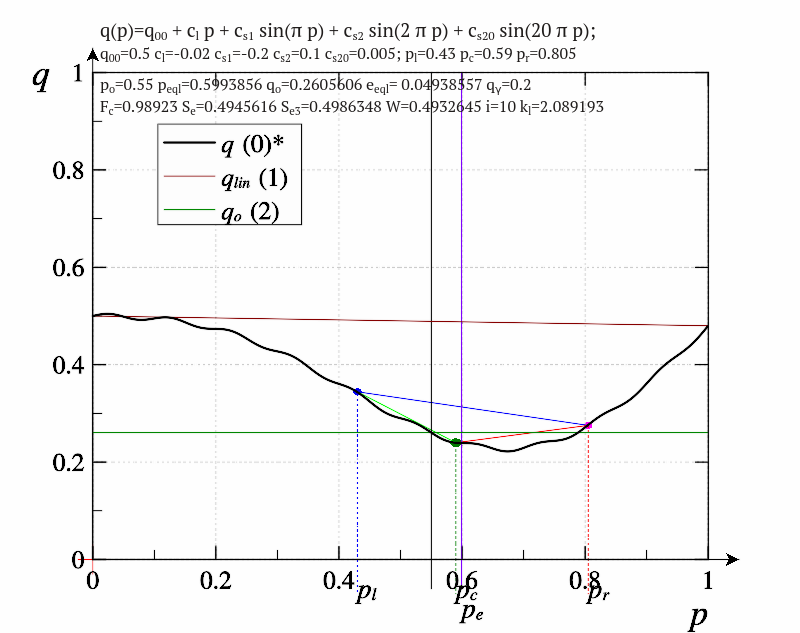
\includegraphics[width=60\TW]{p/pq_sin-p_pq_double.png} }
  \caption{Конфигурация точек, соответствующая случаю 3}
  \label{atu:f:pq_3}
\end{figure}

Это достаточно нетривиальный случай,
и при правильном критерии и идеальных условиях
встречаться не должен. Однако, в реальных условиях,
при наличии ошибок изменения и несовершенстве критерия
данный случай вполне возможен (пусть и достаточно редко), и требует отдельной обработки.
Более того, в отличие от неопределённых случаев 2A и 2C,
данный свидетельствует о том, что искомое значение
действительно лежит в текущем рабочем диапазоне,
но помехи и нелинейности не дают возможности установить его
точное положение. При этом, если для определения $p_e$
выбрать один из интервалов $[p_l,p_c]$ и $[p_c, p_r]$,
то этот выбор, с учётом помех, будет практически случайным,
и малые изменения в значениях критерия могут переключить на другую ветвь.
Поэтому, для определения $p_e$ используем подход, аналогичный применённому
в случае 2A, но с другими коэффициентами:
%
\begin{equation}
  \tilde{p}_e = 0.1 ( \tilde{p}_{el} + \tilde{p}_{er} ),
  \;
  c_\mathrm{su} = 0.5, \;  c_\mathrm{dist} = 2, \;   p_b = \frac{p_r - p_l}{2}.
  \label{atu:eq:pr_e_3}
\end{equation}


\paragraph{Случай 4.}
Дві послідовні точки
розташовані по один бік
від прямої
$q = q_o$, а решта --- по інший, тобто в робочому діапазоні існує тільки один
корінь~(рис.~\ref{atu:f:pq_4}).


\begin{figure}[htb!]
  \centerline{
    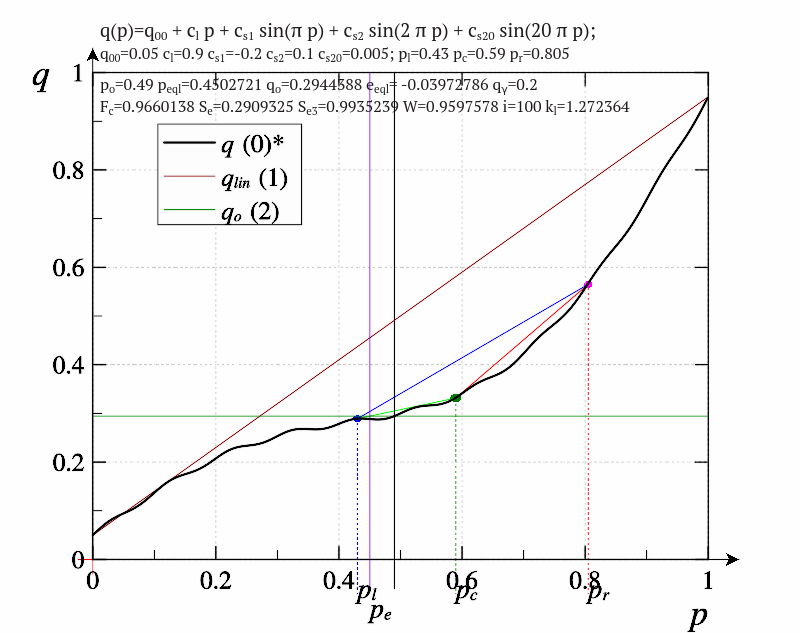
\includegraphics[width=49\TW]{p/pq_sin-p_pq_po=049.png}
    \hfill
    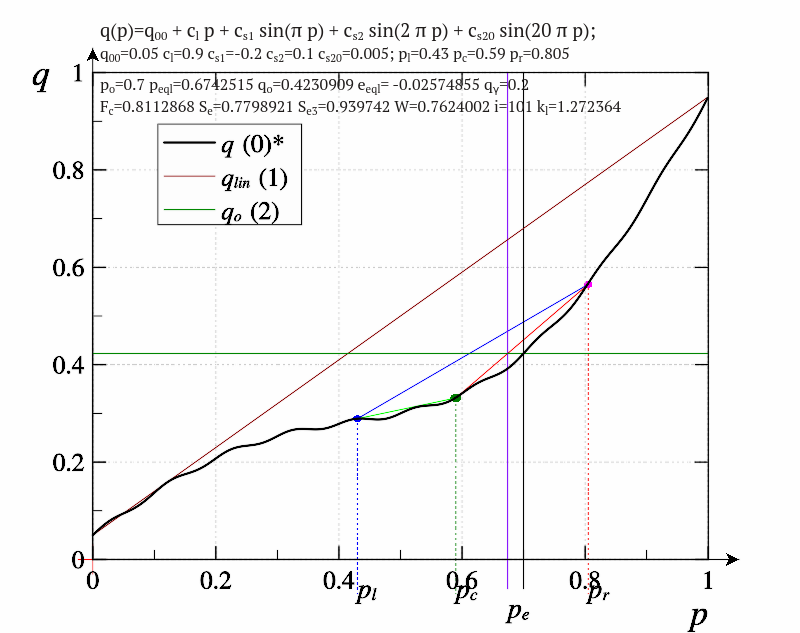
\includegraphics[width=49\TW]{p/pq_sin-p_pq_po=070.png}
  }
  \caption{Конфигурации точек, соответствующие случаю 4}
  \label{atu:f:pq_4}
\end{figure}

У цьому найсприятливішому випадку проводиться інтерполяція, а не екстраполяція
залежності $q(p)$, і досить вибрати ту ділянку, на якій гарантовано
відбувається перетин. При цьому значення всіх коефіцієнтів підкреслюють
впевненість агента в значенні $p_e$, що отримано:
%
\begin{equation}
  \tilde{p}_e
  =
  \begin{cases}
    \tilde{p}_{el}, & \tilde{q}_l < 0
    \\
    \tilde{p}_{er}, & \text{ otherwise}.
  \end{cases}
  ,
  c_\mathrm{su} = 1.0, \;  c_\mathrm{dist} = 0.5,  \;
  p_b =
  \begin{cases}
    -\tilde{p}_l, & \tilde{q}_l < 0
    \\
    \tilde{p}_r, & \text{ otherwise}.
  \end{cases}.
  \label{atu:eq:pr_e4}
\end{equation}

У будь-якому з розглянутих випадків, має сенс ввести додаткове обмеження на
значення $p_e$, так як через похибки вимірювання і моделювання воно може
виявитися навіть поза діапазону $[p_{\min}, p_{\max}]$. З практичної
точки зору досить добре зарекомендувало себе обмеження
$\tilde {p}_r \in [2 \tilde{p}_l, 2 \tilde{p}_r]$.
З урахуванням низького значення $S$ для
агентів, які потрапили під таке обмеження, їх вплив на загальний результат буде
мінімальним, так як нормальному перебігу процесу ідентифікації існує хоча б
один агент з високим значенням $S$. Більш суворі обмеження досить рідко
виправдовують себе, так як при цьому не використовуються екстраполяційні
властивості агентів.

Описаний даними правилами спосіб визначення $p_e$ в подальшому будемо
означати як $p_{eql}$\label{atu:d:p_eql}.

\paragraph{Учёт влияния оценки линейности зависимости $q(p)$}

В предшествующих рассуждениях при вычислении коэффициента ``уверенности'' $S$
в расчёт принималось только расстояние от текущих значений параметров модели для $p_e$.
При этом не учитывалась возможность оценки линейности аппроксимации $q(p)$
по имеющимся данным. При этом оценка должна быть независима от изменения масштаба
как параметров, так и критериев, иметь удобную форму для дальнейшего
использования, и не требовать вычислений, сильно чувствительным к помехам измерений.

Так как в рассматриваемом случае один агент наблюдает значения $p$ и $q$
для трёх моделей, то оценить влияние нелинейных факторов он может
следующим образом. В первую очередь, по значениям, соответствующим крайним точкам
линейной интерполяцией оценивается значение $q_c$ (или же после нормализации --- $\tilde{q}_c$):
%
\begin{equation}
 q_{c,\mathrm{lin}}
  =
  \frac{  q_l \left( p_r - p_c \right) + q_r \left( p_c - p_l \right) }{p_r-p_l},
  \label{atu:eq:q_clin}
\end{equation}
%
\begin{equation}
  \tilde{q}_{c,\mathrm{lin}}
  =
  \frac{ \tilde{q}_l \tilde{p}_r - \tilde{q}_r \tilde{p}_l }{\tilde{p}_r-\tilde{p}_l}  .
  \label{atu:eq:qr_clin}
\end{equation}

Для обеспечения корректности и малой чувствительности полученных оценок
к ошибкам измерения следует обеспечить достаточное расстояние между соседними агентами.
Это требование необходимо учитывать при определении динамики агентов.
С другой стороны, проведении всех предыдущих оценках величины $p_e$
неявно предполагалось $\tilde{p}_l < 0$ и $\tilde{p}_r > 0$.
Следовательно, на начальном этапе работы метода случай чрезмерной близости агентов
детектироваться автоматически и обрабатываться отдельно особым образом.
Например, в этом случае имеет смысл принять $p_e = p_c$
при сохранении достаточно высоких значений $S$ --- если метод привёл
несколько агентов в малую окрестность одной точки, то
или точка действительно близка к искомой, или же весь метод
недостаточно пригоден для решения поставленной задачи.


Из полученных оценок $q_{c,\mathrm{lin}}$, $\tilde{q}_{c,\mathrm{lin}}$
сформируем следующие безразмерные коэффициенты, позволяющие оценить
нелинейность $q(p)$:
%
\begin{equation}
  k_l = 1 + \frac{|q_c - q_{c,\mathrm{lin}}|}{|q_r-q_l|} ,
  \label{atu:eq:k_l1}
\end{equation}
%
\begin{equation}
  k_l = 1 + \frac{|\tilde{q}_c - \tilde{q}_{c,\mathrm{lin}}|}{ |\tilde{q}_r-\tilde{q}_l|} .
  \label{atu:eq:k_l2}
\end{equation}

Данное представление $k_l$ было выбрано с целью непосредственного использования
этой величины в $S$, т.е. если $\tilde{q}_{c,\mathrm{lin}} \to \tilde{q}_c$,
то $k_l \to 1$, и есть основания полагать, что на расстояниях порядка $p_r-p_l$
оценка $p_e$ достаточно состоятельна. С другой стороны,
если $k_l \gg 1 $, то нелинейные эффекты в рассматриваемой области
преобладают над линейными, и оценку $p_e$  стоит рассматривать как недостоверную.
При практическом использовании имеет смысл искусственно ограничить эту величину,
например $k_l < 100 $, так как неограниченный рост при стремлении знаменателя
к нулю принципиально ничего не меняет в работе метода, но при этом
возможны проблемы чисто вычислительного характера.





% }}}2

\subsection{Методы агентов, использующих значения функции качества }  % {{{2

Єдиний нерухомий агент, який використовує значення функції якості, ще більш марний (з
точки зору синтезу системи ідентифікації), ніж один нерухомий агент, який
використовує значення критерію.
%
так как в этом случае даже наличие
зависимости $q(p)$ не даёт возможности однозначно определить
значение параметра.
Он может сигнализировать о том, что в пределах
\(\tau\) модель была или не была достаточно адекватна
объекту.

Наличие истории и возможность перемещаться дают возможность
построить систему идентификации и на одном агенте.
В качестве истории могут использоваться, в том числе,
динамические свойства идентифицируемого объекта
(оригинальный метод АПИ). Также могут быть
применены интегрирующие элементы агента идентификации
(синхронный детектор, \ldots).

У найпростіших випадках можлива побудова системи ідентифікації з однією моделлю
і, відповідно, одним пошуковим агентом.
%
Примерами такого похода могут служить
метод синхронного детектора \cite{adopt_cont_sys}
и оригинальный адаптивно-поисковый метод \cite{mich_92}.
Применение методов с одной моделью требует определённого механизма
сохранения истории процесса поиска, по крайней мере в пределах
одного поискового ``периода''. Это сильно ограничивает диапазон
применимости данных методов, в первую очередь --- из-за значительных
временных затрат на повторяющийся поиск.

Применение пары моделей \cite{atu_asau3} % \Cmt{figure, or link to p1?}
(в этом случае имеет смысл говорить об одном поисковом агенте)
позволяет с меньшими временными затратами оценить градиент функции качества,
и, как следствие --- определить значение параметра. Также значительным преимуществом
такого подхода является меньшая скорость изменения параметров моделей.


Пара агентів, що взаємодіє між собою, здатна оцінити градієнт функції якості,
і, отже, забезпечити зміщення в потрібному напрямку.

С учетом глобальной информации возможна адаптация параметров пары.
В свою очередь, информация, полученная от пары может
использоваться для уточнения глобальных параметров.


Кожен пошуковий агент, визначаючи величину $q_{i}(t)$, і отримуючи $q_o(t)$,
обчислює безрозмірну функцію якості ідентифікації $F (q_o, q_i)$. Як
варіант, агент (або навіть вся керована частина системи ідентифікації) не має
безпосереднього доступу до критерію, і отримує власне значення~$F$.

Три сусідніх агента, які взаємодіють між собою, здатні не тільки оцінити градієнт
функції якості у власному околі, а й визначити наявність там
максимуму.

На відміну від методів, які використовують значення критерію безпосередньо, в
цьому випадку немає можливості обробляти кожну з пар точок $(p_l, p_c)$ і
$(p_c, p_r)$ незалежно. З трьох точок поблизу $M_{i}$ функція $F(p)$
апроксимується параболою, і абсциса її вершини задає шукане значення параметра.
Змістимо початок координат в точку
$(p_c, F_c)$. Тоді
%
\[
  \tilde{p}_c = 0, \,
  \tilde{p}_l = p_l - p_c, \,
  \tilde{p}_r = p_r - p_c.
\]
%
\[
  \tilde{F}_c = 0, \,
  \tilde{F}_l = F_l - F_c, \,
  \tilde{F}_r = F_r - F_c.
\]
%
\[
  \left\{
    \begin{array}{l}
      a_2 \tilde{p}_l^2 + a_1 \tilde{p}_l  = \tilde{F}_l
      \\
      a_2 \tilde{p}_r^2 + a_1 \tilde{p}_r  = \tilde{F}_r
    \end{array}
  \right. .
\]
%
\[
  a_1 = \frac{\tilde{F}_r \tilde{p}_l^2 - \tilde{F}_l \tilde{p}_r^2 }
             { \tilde{p}_l^2 \tilde{p}_r  - \tilde{p}_l \tilde{p}_r^2 }.
\]
%
\[
  a_2 = - \frac{\tilde{F}_r \tilde{p}_l - \tilde{F}_l \tilde{p}_r }
               { \tilde{p}_l^2 \tilde{p}_r  - \tilde{p}_l \tilde{p}_r^2 }.
\]

\begin{equation}
  \tilde{p}_e = - \frac{a_1}{2 a_2};
  \;
  p_e = p_c - \frac{a_1}{2 a_2}.
  \label{atu:eq:p_eFq}
\end{equation}

При цьому, якщо
$a_2 \ge 0$,
то ця ситуація аналогічна випадку 2C метода $p_{eql}$~(см.~стр.~\pageref{atu:d:p_eql_2A}),
що потребує обмеження $p_e$ та корекції величин $c_\mathrm{su}$ та $c_\mathrm{dist}$.

Визначення $p_e$ по (\ref{atu:eq:p_eFq}) будемо позначати як $p_{eFq}$.

Определение $p_e$ по (\ref{atu:eq:p_eFq}) будем обозначать $p_{eFq}$.

Рассмотрим работу этого метода при тех же условиях,
при которых иллюстрировался метод $p_{eql}$.
Прежде всего проиллюстрируем вариант,
когда центральная точка --- наихудшая~(рис.~\ref{atu:f:p_eFq_bad}).


\begin{figure}[htb!]
  \centerline{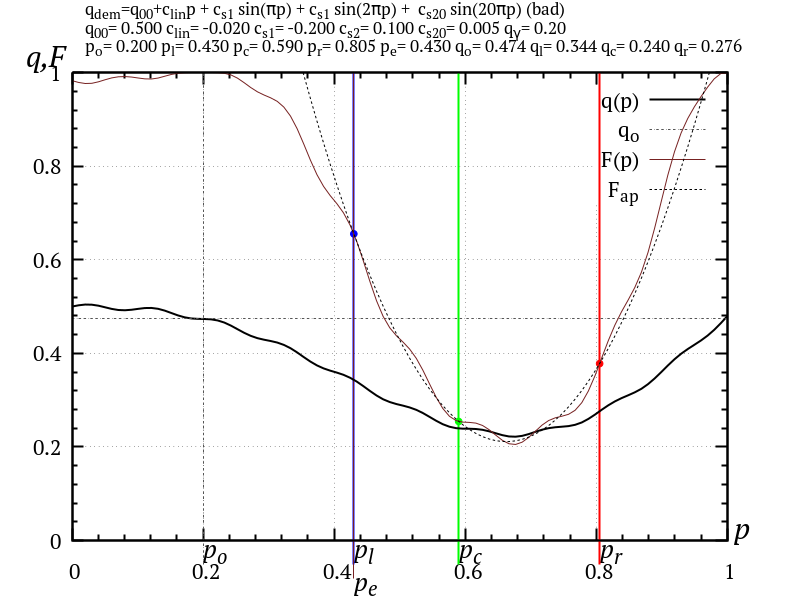
\includegraphics[width=60\TW]{p/p_eFq/q_p_eFq_bad.png}}
  \caption{Определение точки $p_e$ методом $p_{eFq}$ в худшем случае}
  \label{atu:f:p_eFq_bad}
\end{figure}

Как видно из графика, в этом случае аппроксимация зависимости $F(p)$
параболой $F_{ap}(p)$ достаточно точная, но положительная определённость величины
$a_2$ показывает, что найденный экстремум соответствует минимуму,
что совершенно не помогает в определении $p_e$. В то же время,
действие метода в этом случае --- выбор одной из граничных точек
правильно указывает направление.

Противоположный случай, когда центральная точка --- наилучшая,
но всё же недостаточно ``хорошая'', представлен на рис.~\ref{atu:f:p_eFq_good}.

\begin{figure}[htb!]
  \centerline{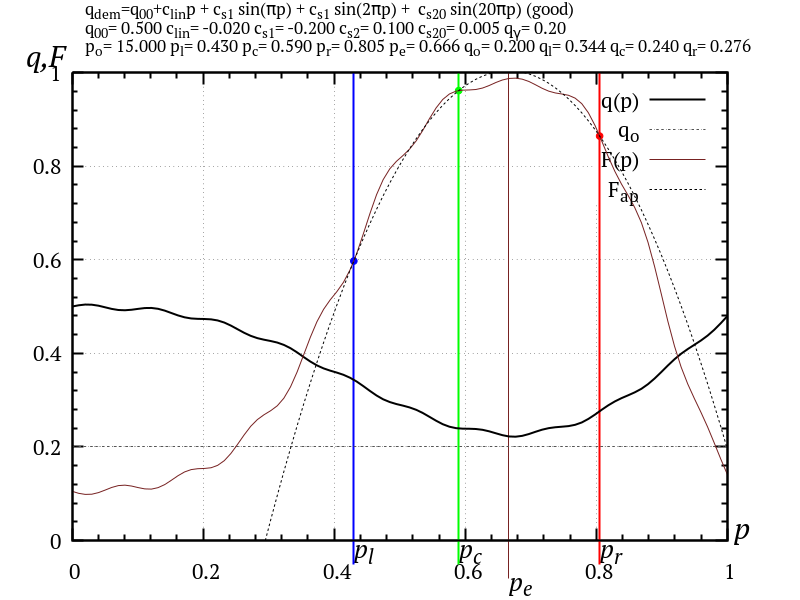
\includegraphics[width=60\TW]{p/p_eFq/q_p_eFq_good.png}}
  \caption{Определение точки $p_e$ методом $p_{eFq}$ в случае, когда центральная точка --- наилучшая, но нет пересечения $q(p)$ с $q_o$ }
  \label{atu:f:p_eFq_good}
\end{figure}

В отличие от метода $p_{eql}$, для рассматриваемого метода
этот случай не является особым. Найденное значение $p_e$
достаточно хорошо соответствует точке, в которой
$q(p)$ максимально приближается к $q_o$. Это вполне разумное поведение,
с учётом того, что при приближении к этой точке, по уточнённым данным
может быть найдено пересечение $q(p) = q_o$. С другой стороны,
это может быть локальный экстремум, не соответствующий искомому значению $p_o$,
как и представлено в этом примере.

Пример неопределённого случая, когда на рабочем интервале есть
два пересечения $q(p)$ с $q_o$, представлен на рис.~\ref{atu:f:p_eFq_double}.

\begin{figure}[htb!]
  \centerline{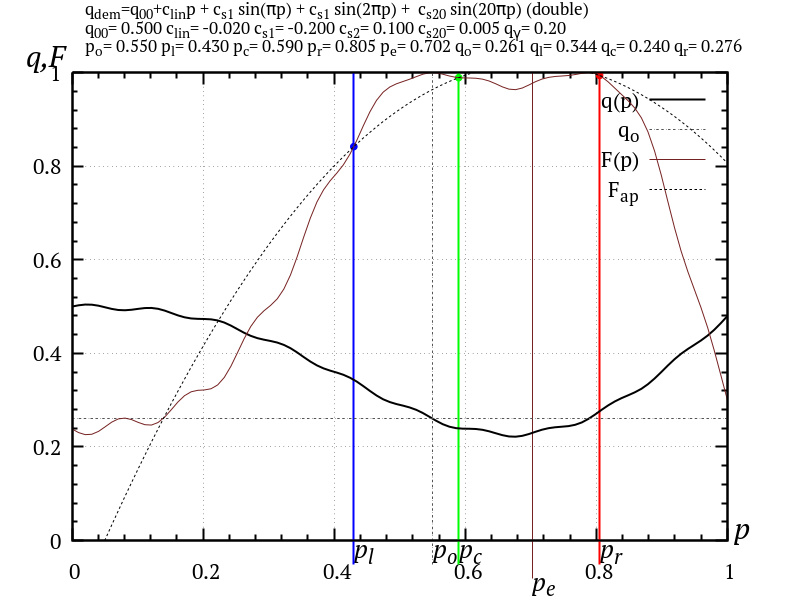
\includegraphics[width=60\TW]{p/p_eFq/q_p_eFq_double.png}}
  \caption{Определение точки $p_e$ методом $p_{eFq}$ в случае двух пересечений $q(p)$ с $q_o$ }
  \label{atu:f:p_eFq_double}
\end{figure}

Неопределённость условия не позволяет выбрать какое-либо определённое и
наилучшее в любом случае поведение. В данном конкретном случае
был выбран вариант, уводящий от исходного $p_o$.
Более того, в отличие от метода $p_{eql}$,
алгоритмически данный случай выделить невозможно, опираясь только на значения
функции качества. Как результат --- нет возможности отметить этот случай снижением
величины $S$.

Рассмотрим более определённый случай, для которого метод $p_{eql}$
получал оценку $p_e$ путём экстраполяции (рис.~\ref{atu:f:p_eFq_extra}).

\begin{figure}[htb!]
  \centerline{
    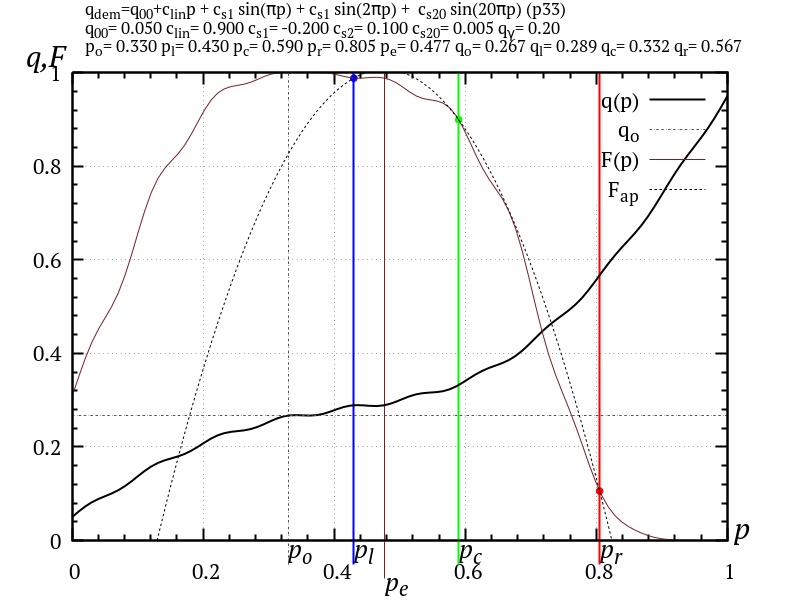
\includegraphics[width=49\TW]{p/p_eFq/q_p_eFq_p33.png}
    \hfill
    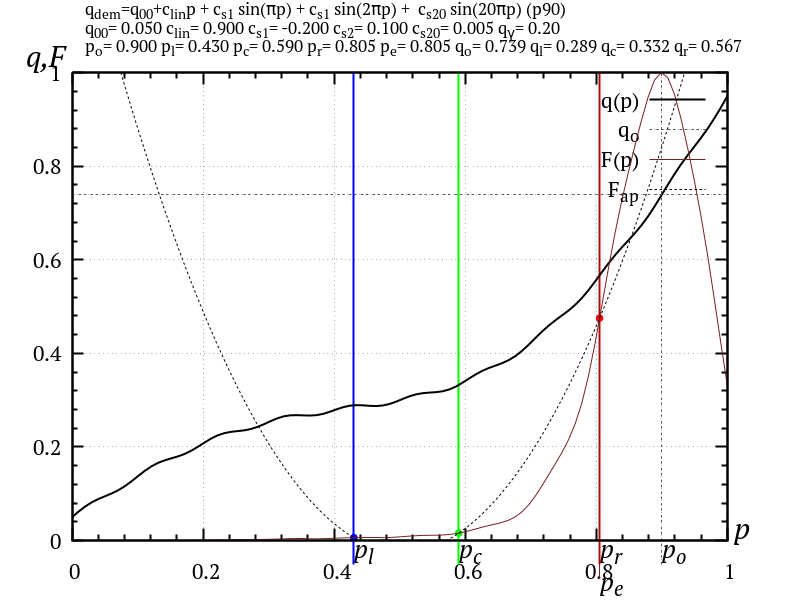
\includegraphics[width=49\TW]{p/p_eFq/q_p_eFq_p90.png}
  }
  \caption{Определение точки $p_e$ методом $p_{eFq}$ при экстраполяции за пределы $[p_l,p_r]$ }
  \label{atu:f:p_eFq_extra}
\end{figure}

Здесь наблюдаются серьёзные отличия от метода $p_{eql}$.
Прежде всего, поведение предыдущего метода
в этом, достаточно простом случае, было достаточно однозначным.
Достаточно было по заданным правилам уменьшать величину $S$
при удалении от рабочего интервала, для отображения
уменьшения степени уверенности в полученном значении.
Данный метод, как видно на представленных графиках,
в сходных случаях может давать совершенно различные результаты.
Первый график, соответствующий $p_o=0.33$,
демонстрирует не только значительную ошибку идентификации,
но и тот факт, что нет возможности отделить этот случай от
наиболее благоприятного, при $p_o \in [p_l,p_r]$.
Второй график ($p_o=0.9$), хотя исходные условия принципиально не отличаются
от первого, реализует условие $a_2 \ge 0 $, т.е. невозможность
определить $p_e$ за счёт аппроксимации второго порядка, и следовательно,
вынуждает в качестве приближения использовать $p_r$.

Метод в найбільш сприятливому випадку, при
$p_o \in [p_l,p_r]$, представлено на рис.~\ref{atu:f:p_eFq_intra}.


\begin{figure}[htb!]
  \centerline{
    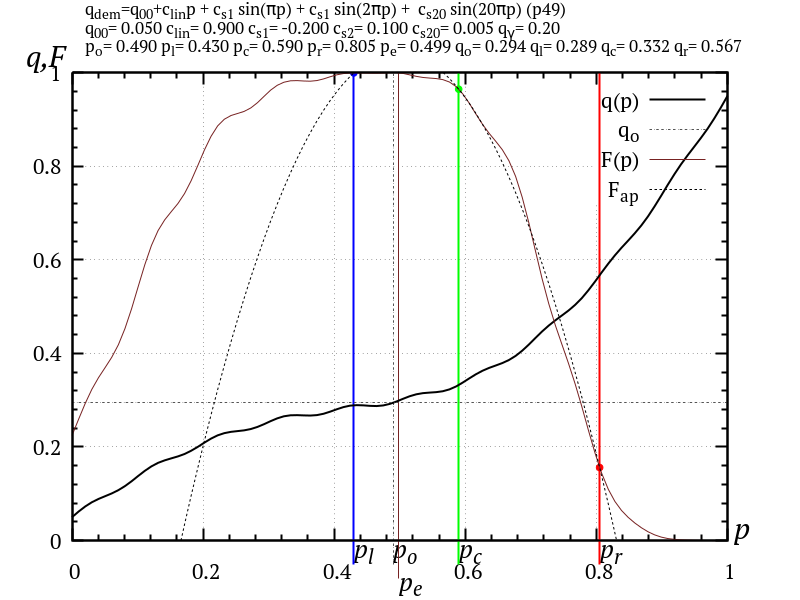
\includegraphics[width=49\TW]{p/p_eFq/q_p_eFq_p49.png}
    \hfill
    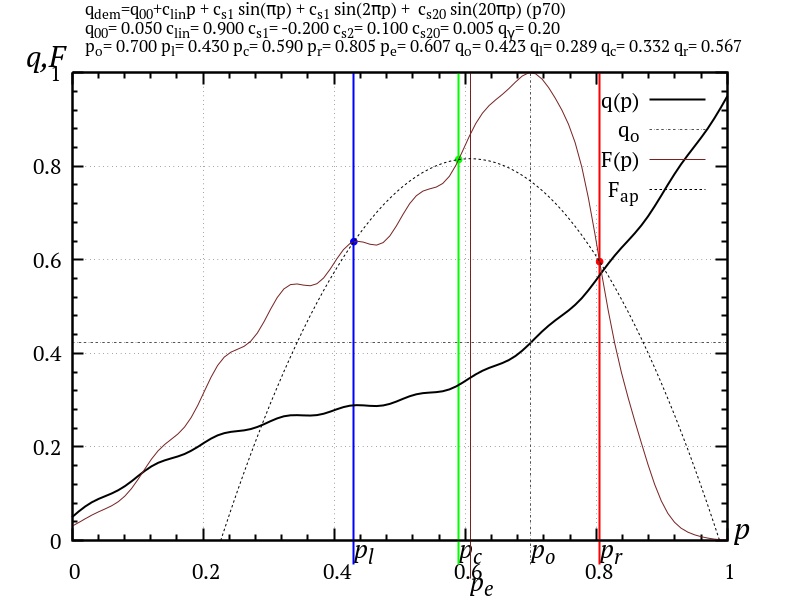
\includegraphics[width=49\TW]{p/p_eFq/q_p_eFq_p70.png}
  }
  \caption{Определение точки $p_e$ методом $p_{eFq}$ при   $p_o \in [p_l,p_r]$}
  \label{atu:f:p_eFq_intra}
\end{figure}

Як і слід було очікувати, оцінка $p_e$ в цьому випадку цілком спроможна, не
дивлячись на те, що в подібних умовах спостерігається різний рівень похибки
ідентифікації.

Рассмотрим влияние на работоспособность рассматриваемого метода
чувствительности функции качества, определяемой величиной $q_\gamma$.
Исходное значение этой величины ($q_\gamma=0.2$) для
тестовой задачи было подобрано экспериментально~\cite{atu_asau22}.
Рассмотрим изменение результатов работы метода в при $p_o \in [p_l,p_r]$
в условиях сильно завышенной чувствительности $q_\gamma=0.05$ (рис.~\ref{atu:f:p_eFq_intra_005}).


\begin{figure}[htb!]
  \centerline{
    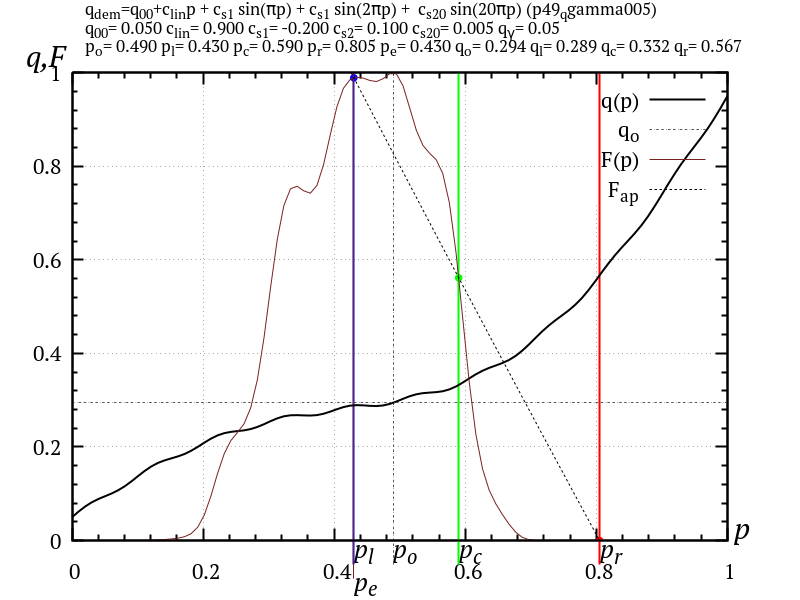
\includegraphics[width=49\TW]{p/p_eFq/q_p_eFq_p49_qgamma005.png}
    \hfill
    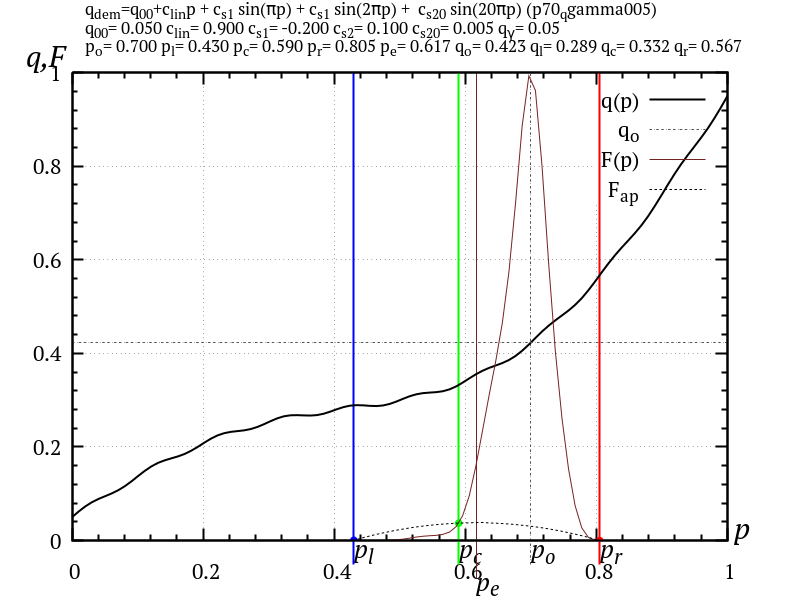
\includegraphics[width=49\TW]{p/p_eFq/q_p_eFq_p70_qgamma005.png}
  }
  \caption{Определение точки $p_e$ методом $p_{eFq}$ при завышенной чувствительности функции качества}
  \label{atu:f:p_eFq_intra_005}
\end{figure}

Цій метод демонструє суттєву чутливість до значення $q_\gamma$.
Зайва чутливість призводить до того, що функція якості є відмінною від нуля в
дуже вузькому діапазоні значень параметра, що призводить до практичної
безглуздості апроксимації і неадекватним результатам
ідентифікації.

Существенно другие результаты показывает метод в условиях
недостаточной чувствительности, то ест при
относительно больших значениях $q_\gamma$ (рис.~\ref{atu:f:p_eFq_intra_200}).

\begin{figure}[htb!]
  \centerline{
    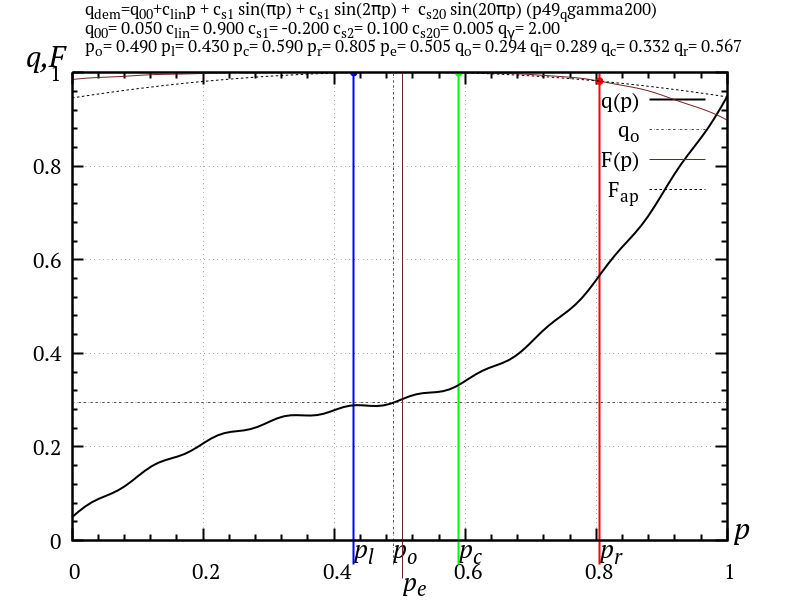
\includegraphics[width=49\TW]{p/p_eFq/q_p_eFq_p49_qgamma200.png}
    \hfill
    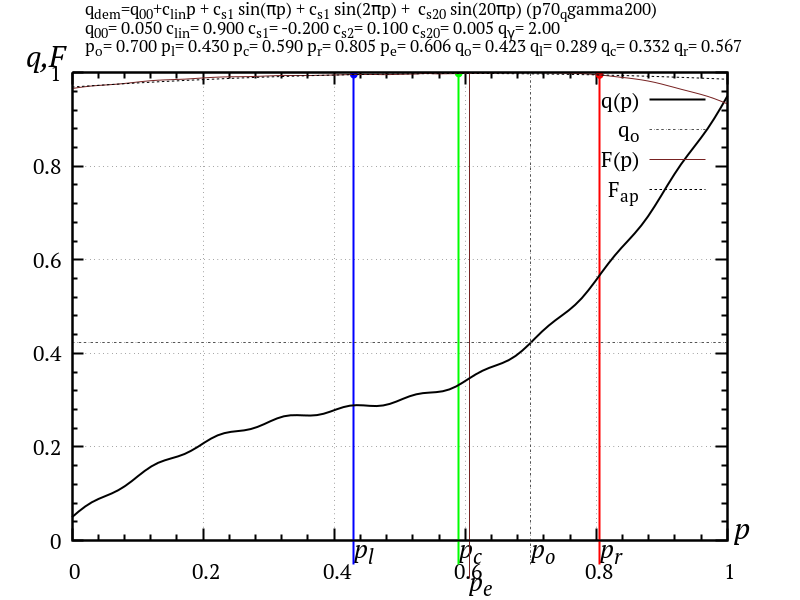
\includegraphics[width=49\TW]{p/p_eFq/q_p_eFq_p70_qgamma200.png}
  }
  \caption{Определение точки $p_e$ методом $p_{eFq}$ при недостаточной чувствительности функции качества}
  \label{atu:f:p_eFq_intra_200}
\end{figure}

Досить дивним є той факт, що при значному зменшенні чутливості похибка
ідентифікації росте дуже слабо. В першу чергу це пов'язано з тим, що в цих
умовах сама апроксимація кривої $F$ параболою стає більш точною. Для інших
видів функції якості це не так. Більш того, наведені приклади розраховувалися
за умови відсутності помилок вимірювання. При недостатній чутливості
$F_l \approx F_c \approx F_r \approx 1$, і малі зміни $F$ приведуть до значної
похибки ідентифікації.

В цілому, на підставі отриманих результатів, даний метод демонструє дещо
гірші результати, ніж $p_{eql}$.
%
Наиболее серьёзным недостатком следует считать
невозможность в произвольном случае достаточно уверенно
определить величину $S$, которая на уровне координатора поиска
позволяет выбрать наиболее значимых агентов, а на уровне агента ---
избежать избыточной динамики вдали от $p_o$.
Вторым по важности недостатком является необходимость
корректной настройки величины $q_\gamma$, пусть и в достаточно широких пределах.
Среди достоинств метода следует отметить более простую
алгоритмическую организацию, что может быть существенно
при реализации системы идентификации в условиях с ограниченным вычислительными
ресурсами.



\paragraph{Определение $p_e$ методом COG по значениям функции качества в 3 точках}

Досить простим і маловитратними з точки зору обчислень є метод оцінювання $p_e$ методом
COG за значеннями функції якості:
%
\begin{equation}
  p_e =
  \frac{p_l F_l + p_c F_c + p_r F_r}{ F_r + F_c + F_r}  .
  \label{atu:eq:p_eFc}
\end{equation}

Умова обмеженості оцінки $p_e \in [p_l; p_r]$ в цьому випадку виконується
автоматично.
%
Единственная сложность --- обработка особого случая для тех видов
$F(q)$, которые обращаются в ноль на удалении от центральной точки.
В этом случае знаменатель (\ref{atu:eq:p_eFc}) обращается в ноль,
в в качестве $p_e$ имеет смысл выбрать $p_c$.
Для тех видов функций качества, которые не принимают строго нулевых
значений, формально такой проблемы нет. Нем не менее,
данное состояние сильно подвержено влиянию помех измерения.

Для этого способа не представляется возможным
достаточно полезным способом определить величину $S$,
поэтому, для сохранения единообразия положим $S=1$.

Визначення $p_e$ по (\ref{atu:eq:p_eFc}) в подальшому будемо позначати $p_{eFc}$.



% }}}2

\subsection{Оценка работоспособности и эффективности методов оценивания идентифицируемого параметра одним поисковым агентом}  % {{{2

Для визначення працездатності і властивостей різних методів оцінювання $p_e$
в контрольованих умовах без урахування динаміки агентів була обрана наступна
тестова задача: залежність $q (p)$ визначалася по (\ref{atu:eq:q_dem}),
$p_{\min}=20$, $p_{\max}=60$,
$q_{00}=7$, $c_\mathrm{lin}=-4.0$.
Початкове розташування агентів рівномірне і штучно зафіксоване:
$p_l=30$, $p_c=40$,  $p_r=50$.

Значения коэффициентов
$c_\mathrm{s1}$, $c_\mathrm{s2}$, $c_\mathrm{s20}$
выбирались по одному из трёх наборов:
%
\begin{equation}
  c_\mathrm{s1} = 0.2, c_\mathrm{s2} = -0.4, c_\mathrm{s20} = 0.02,
  \label{atu:eq:q_dem_all}
\end{equation}
%
\begin{equation}
  c_\mathrm{s1} = 0, c_\mathrm{s2} = 0, c_\mathrm{s20} = 0.02,
  \label{atu:eq:q_dem_s20}
\end{equation}
%
\begin{equation}
  c_\mathrm{s1} = c_\mathrm{s2} = c_\mathrm{s20} = 0 .
  \label{atu:eq:q_dem_lin}
\end{equation}

При этом набор параметров (\ref{atu:eq:q_dem_all})
позволяет исследовать поведение ошибки идентификации при
влиянии как низкочастотных, так и высокочастотных
нелинейных компонент,
(\ref{atu:eq:q_dem_s20}) --- только высокочастотных,
а (\ref{atu:eq:q_dem_lin}) представляет собой
простейший линейный случай.

\begin{figure}[htb!]
  \centerline{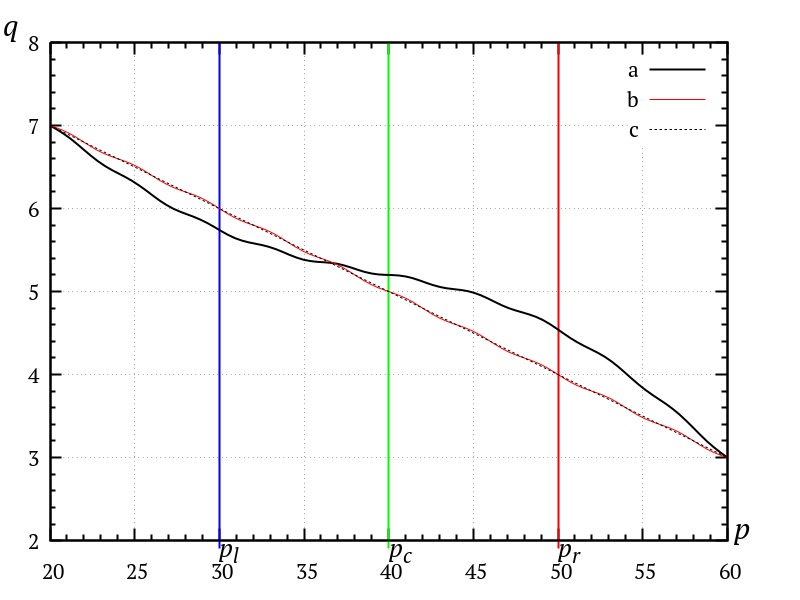
\includegraphics[width=0.7\textwidth]{p/q_p_dem.png} }
  \caption{Вид тестовой функции $q_\mathrm{dem}(p)$:
     a --- условия (\ref{atu:eq:q_dem_all}),
     b --- условия (\ref{atu:eq:q_dem_s20}),
     c --- условия (\ref{atu:eq:q_dem_lin})
  }
  \label{atu:f:q_dem}
\end{figure}

У першій серії обчислювальних експериментів значення параметра об'єкта $p_o$
змінювалося в діапазоні $[p_{\min}; p_{\max}]$ при фіксованій відстані
між агентами $A = p_c - p_l = p_r - p_c$. Це дозволило оцінити як
інтерполяційні (при $p_o \in [p_l, p_r]$), так і екстраполяційні можливості
методів. Так як частина методів при визначенні $p_e$ використовує значення
функції якості, то при проведенні експериментів величина $q_\gamma$ також
варіювалася.

Для метода $p_{eql}$ непосредственной зависимости от этой величины нет,
но для единообразия представленных результатов
все графики приведены как зависимости от $p_o$ и $q_\gamma$.
Все представленные графики, для удобства сравнения,
выполнены в одном масштабе и одной и той же проекции.
Масштаб по оси $Z$, использующейся для представления
модуля ошибки идентификации, был выбран $Z_{\max} = A/2 = 5$
для наглядного сравнения с расстоянием между агентами,
при этом величины, большие $A/2$ соответствуют
неоправданно большой ошибке, и находятся за пределами графика.

На рис.~\ref{atu:f:qsl_pe_po_qg_all} подані залежності помилок
ідентифікації для тестового завдання (\ref{atu:eq:q_dem}) при повному
комплекті нелінійних членів  трьома нерухомими
агентами трьома розглянутим методами визначення $p_e$.

\begin{figure}[htb!]
  \centerline{
    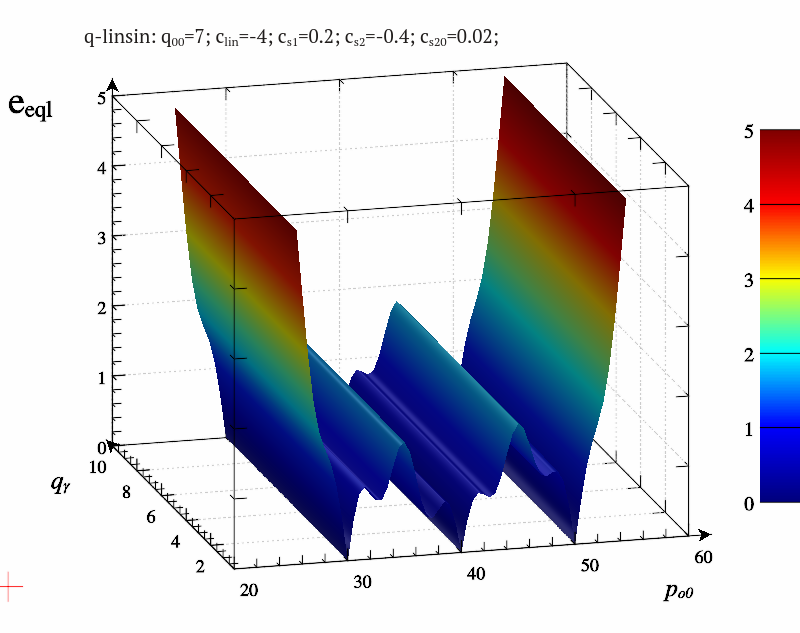
\includegraphics[width=0.32\textwidth]{p/qls_pe-p_po_qg_eql_all.png}
    \hfill
    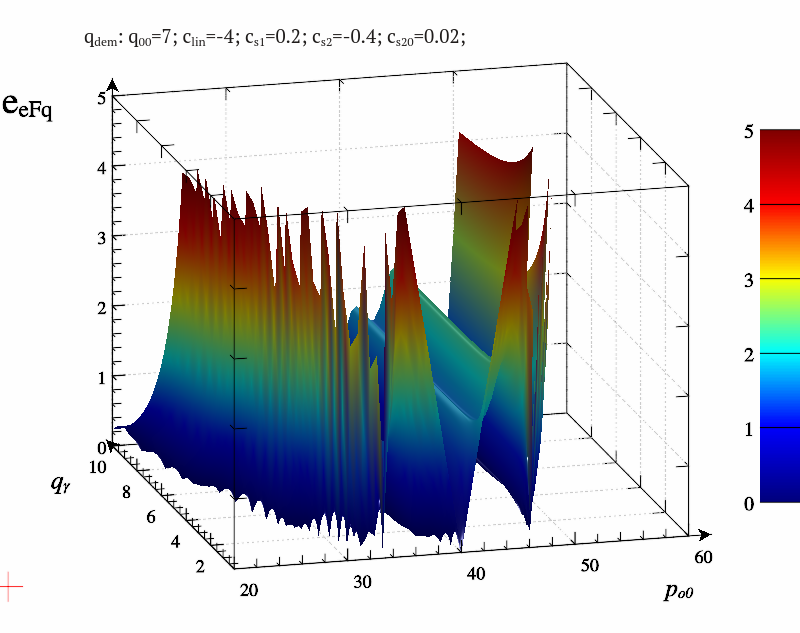
\includegraphics[width=0.32\textwidth]{p/qls_pe-p_po_qg_eFq_all.png}
    \hfill
    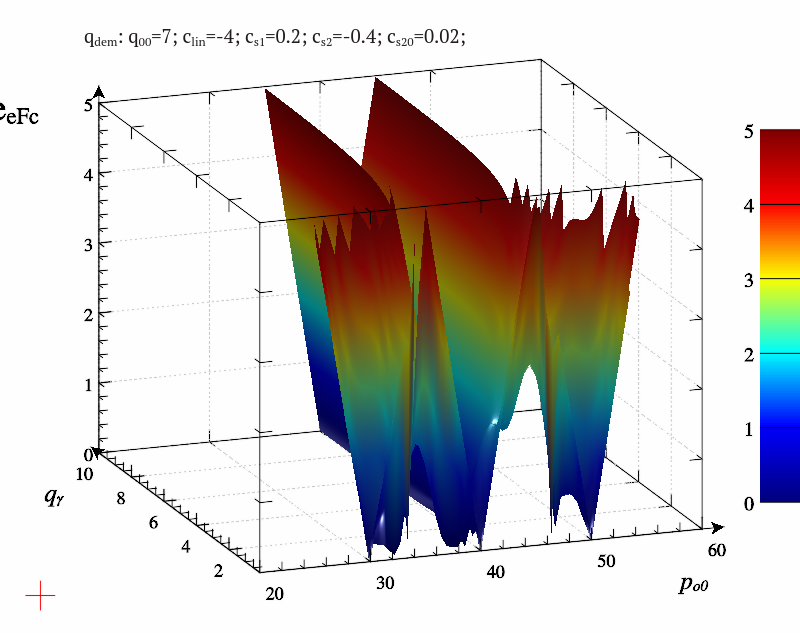
\includegraphics[width=0.32\textwidth]{p/qls_pe-p_po_qg_eFc_all.png}
  }
  \caption{Зависимости $e(p_o,q_\gamma)$ для методов $p_{eql}$, $p_{eFq}$, $p_{qFc}$ для условий (\ref{atu:eq:q_dem_all})}
  \label{atu:f:qsl_pe_po_qg_all}
\end{figure}

Метод $p_{eql}$ демонструє досить обмежену похибку ідентифікації при
$p_o \in [p_l; p_r]$, і досить швидке, але лінійно обмежене зростання похибки за
межами цього робочого діапазону. Метод $p_{eFq}$ має істотну залежність
від величини $q_\gamma$: малі значення призводять до суттєвого
зростання похибки, а з подальшим зростанням рівень похибки в межах робочого
діапазону приблизно одного порядку з похибкою в методі $p_{eql}$. При
цьому, за межами робочого діапазону спостерігається більш суттєве зростання
похибки. Метод $p_{qFc}$ демонструє задовільні результати тільки в дуже
вузькому діапазоні значень $q_\gamma$, що ставить під серйозний сумнів
можливість застосування цього методу для реальних завдань, оскільки при цьому
немає можливості передбачити таке значення цього параметра, при якому метод буде
працездатний.


На рис.~\ref{atu:f:qsl_pe_po_qg_s20} представлены аналогичные зависимости ошибок идентификации,
но из нелинейных членов оставлен самый высокочастотный (\ref{atu:eq:q_dem_s20}).

\begin{figure}[htb!]
  \centerline{
    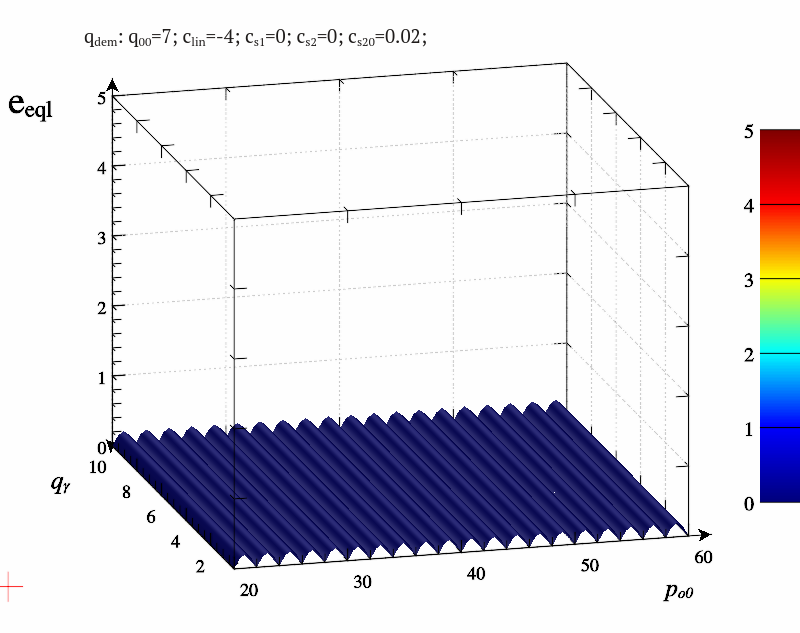
\includegraphics[width=0.32\textwidth]{p/qls_pe-p_po_qg_eql_s20.png}
    \hfill
    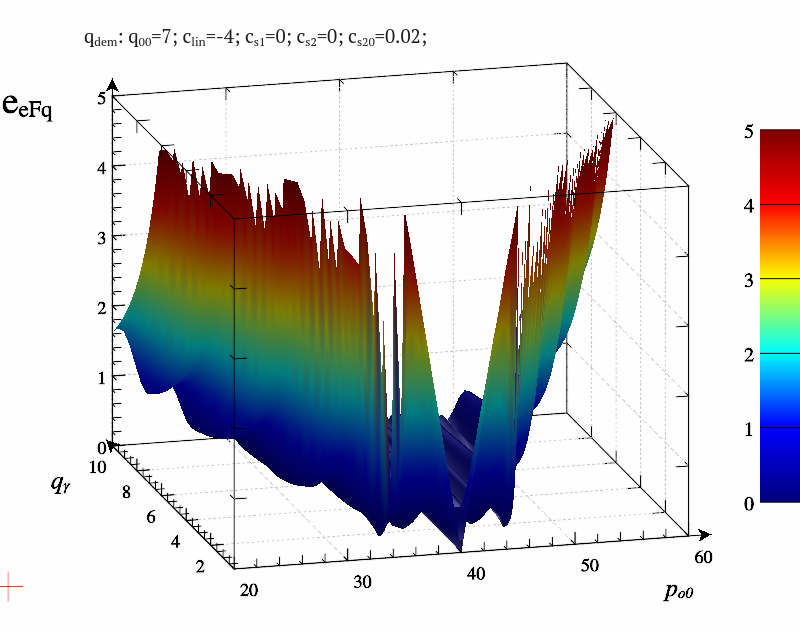
\includegraphics[width=0.32\textwidth]{p/qls_pe-p_po_qg_eFq_s20.png}
    \hfill
    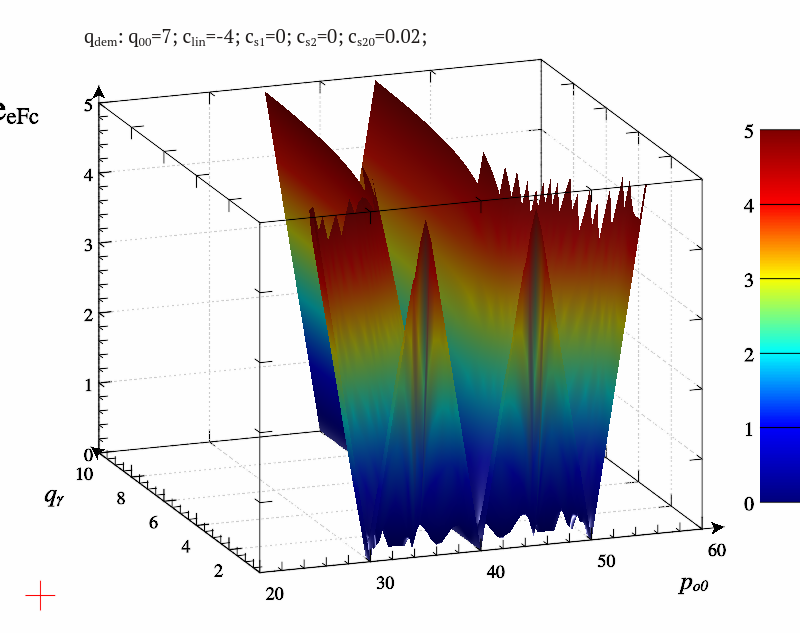
\includegraphics[width=0.32\textwidth]{p/qls_pe-p_po_qg_eFc_s20.png}
  }
  \caption{Зависимости $e(p_o,q_\gamma)$ для методов $p_{eql}$, $p_{eFq}$, $p_{qFc}$ для условий (\ref{atu:eq:q_dem_s20})}
  \label{atu:f:qsl_pe_po_qg_s20}
\end{figure}

В этих условиях метод $p_{eql}$ демонстрирует результаты, близкие к идеальным,
мелкая ``рябь'' на поверхности ошибки соответствует малым периодическим
возмущением $q(p)$, а в целом даже экстраполяция по приводит к росту ошибки.
В какой-то мере это обусловлено тем, что на рабочий диапазон приходится целое
число периодов возмущения. Зависимость ошибки для метода
$p_{eFq}$ проявляет меньшее значение ошибок для
тех участков, где и наблюдался небольшой уровень ошибок для
предыдущего случая, и практически неизменный --- в остальной области.
Принципиальной разницы в поведении метода $p_{qFc}$
по сравнению с предыдущим случаем нет.

На рис.~\ref{atu:f:qsl_pe_po_qg_lin} представлены те же зависимости,
в тривиальном случае (\ref{atu:eq:q_dem_lin}),
когда зависимость $q(p)$ линейна.

\begin{figure}[htb!]
  \centerline{
    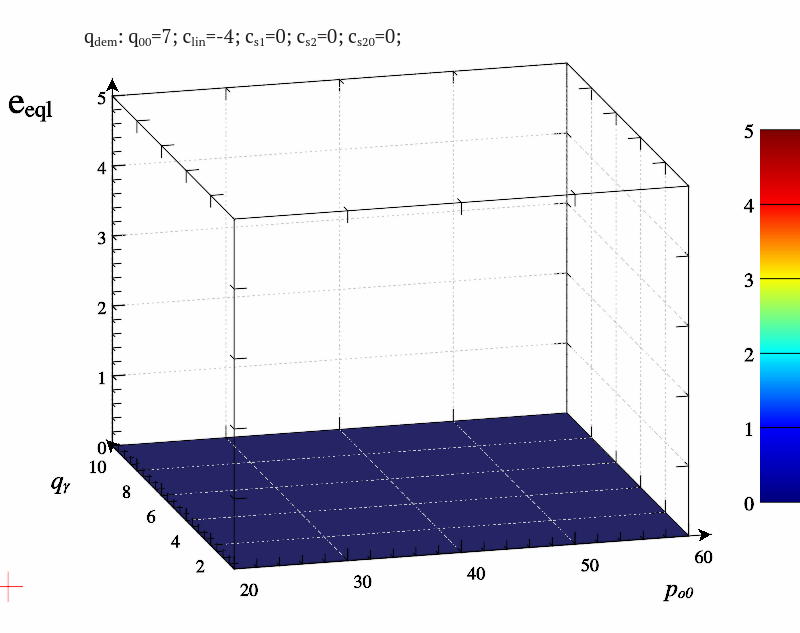
\includegraphics[width=0.32\textwidth]{p/qls_pe-p_po_qg_eql_lin.png}
    \hfill
    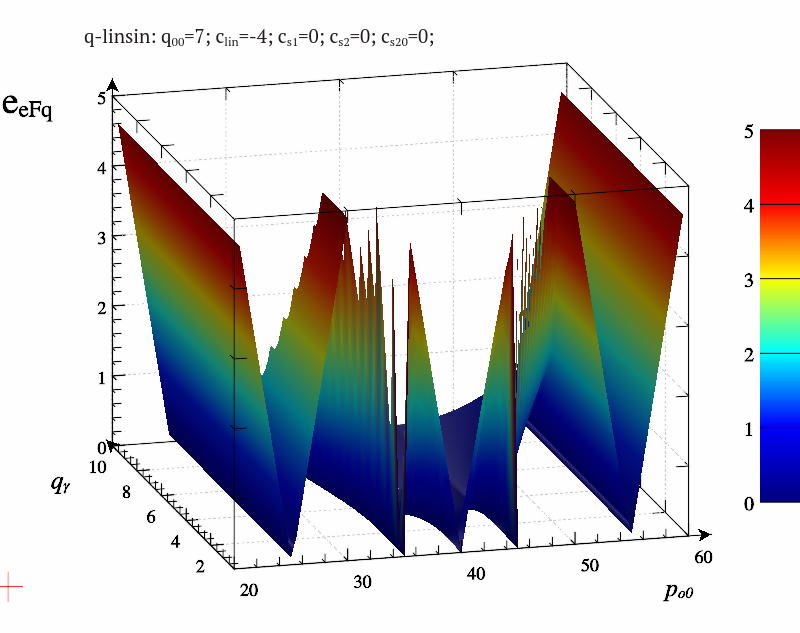
\includegraphics[width=0.32\textwidth]{p/qls_pe-p_po_qg_eFq_lin.png}
    \hfill
    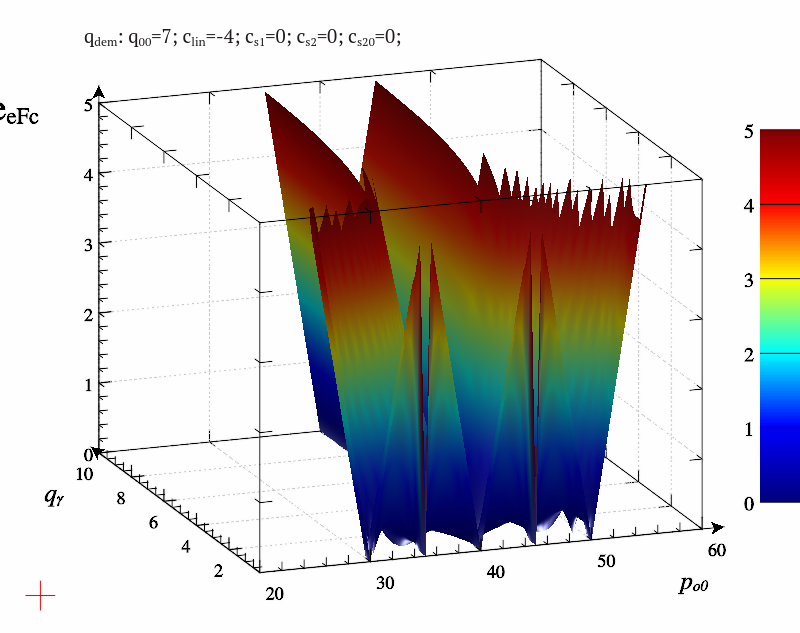
\includegraphics[width=0.32\textwidth]{p/qls_pe-p_po_qg_eFc_lin.png}
  }
  \caption{Зависимости $e(p_o,q_\gamma)$ для методов $p_{eql}$, $p_{eFq}$, $p_{qFc}$ для условий (\ref{atu:eq:q_dem_lin})}
  \label{atu:f:qsl_pe_po_qg_lin}
\end{figure}

Как и следовало ожидать, метод $p_{eql}$
демонстрирует идеальные результаты.
График зависимости для метода $p_{eFq}$
очерчивает его диапазон применимости --- несмотря
на линейность $q(p)$ метод становится неработоспособным при
излишне чувствительной функции качества.
И наконец, поверхность графика для метода $p_{eFc}$,
практически одинаковая для всех рассмотренных вариантов,
подтверждает его слабую применимость.


На рис.~\ref{atu:f:qsl_S_po_qg_all} подані залежності
$S (p_o, q_\gamma)$
при тих же умовах, при яких було отримано рис.~\ref{atu:f:qsl_pe_po_qg_all}.
Використовувалося визначення (\ref{atu:eq:S3}), як
потенційно більш адекватне помилці ідентифікації.

\begin{figure}[htb!]
  \centerline{
    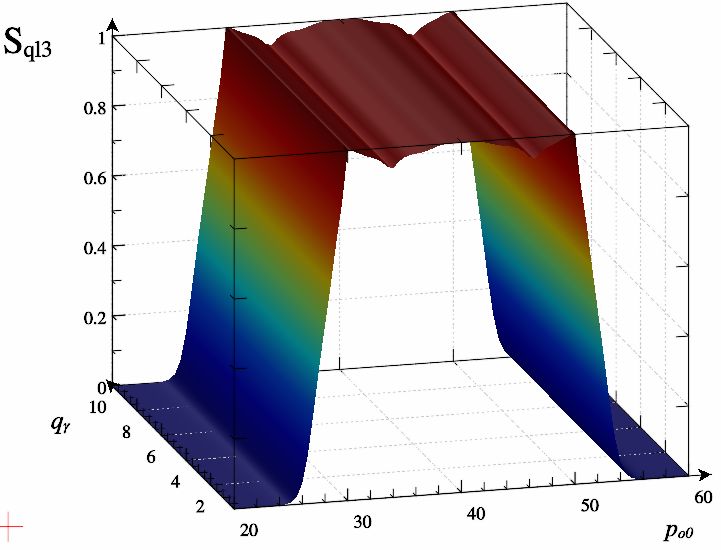
\includegraphics[width=0.32\textwidth]{p/qls_pe-p_po_qg_Sql_all_xl.png}
    \hfill
    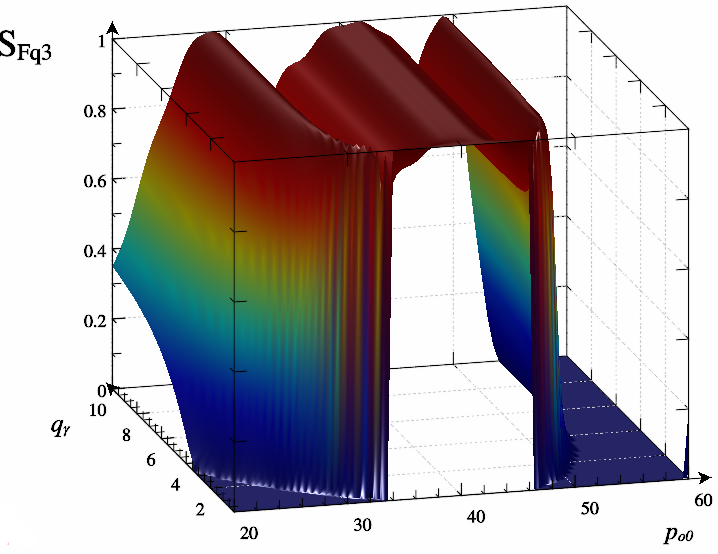
\includegraphics[width=0.32\textwidth]{p/qls_pe-p_po_qg_SFq_all_xl.png}
    \hfill
    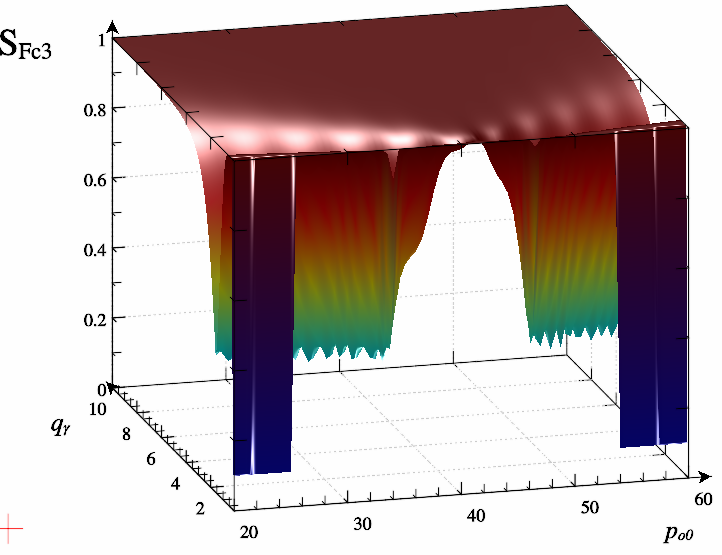
\includegraphics[width=0.32\textwidth]{p/qls_pe-p_po_qg_SFc_all_xl.png}
  }
  \vspace{-1.5ex}
  \begin{center}
    ~ \hfill a \hfill\hfill b \hfill\hfill c \hfill ~
  \end{center}
  \vspace{-2.5ex}
  \caption{Залежності $S(p_o,q_\gamma)$ для методів $p_{eql}$ (a), $p_{eFq}$ (b), $p_{qFc}$(c) при умовах (\ref{atu:eq:q_dem_all})}
  \label{atu:f:qsl_S_po_qg_all}
\end{figure}

Для методу $p_{eql}$ близькі до одиниці значення $S$, як і планувалося,
спостерігаються в тих же областях, де і низький рівень похибки ідентифікації, в
першу чергу --- всередині робочого діапазону. При цьому, ця величина не є
прямим відображення рівня похибки, оскільки це неможливо визначити за трьома точкам.
Метод $p_{eFq}$ також характеризується досить коректним видом цієї залежності,
включаючи низький рівень впевненості при підвищеній чутливості функції якості.
Навпаки, для методу $p_{eFc}$ графік показує, що для нього це визначення $S$ не має сенсу.


На рис.~\ref{atu:f:qsl_S_po_qg_s20} представлены аналогичные зависимости,
но из нелинейных членов оставлен самый высокочастотный (\ref{atu:eq:q_dem_s20}).

\begin{figure}[htb!]
  \centerline{
    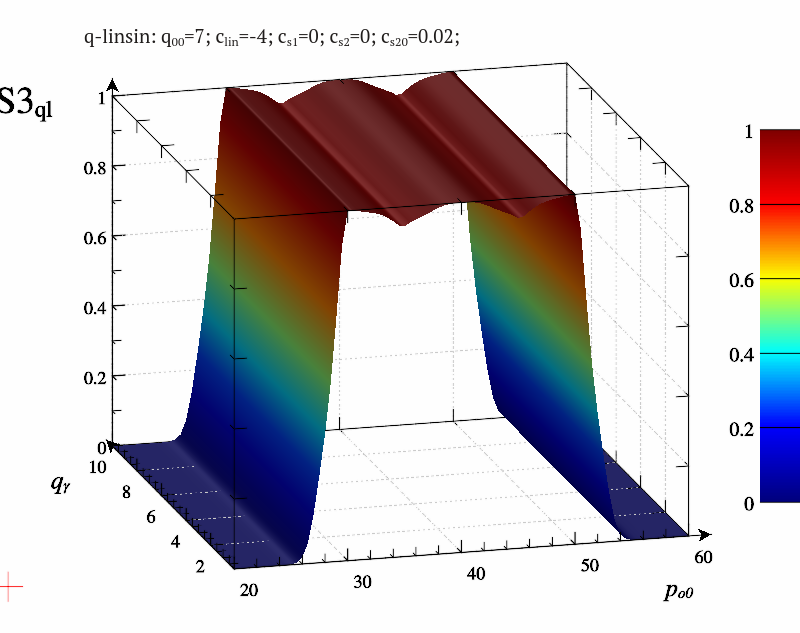
\includegraphics[width=0.32\textwidth]{p/qls_pe-p_po_qg_Sql_s20.png}
    \hfill
    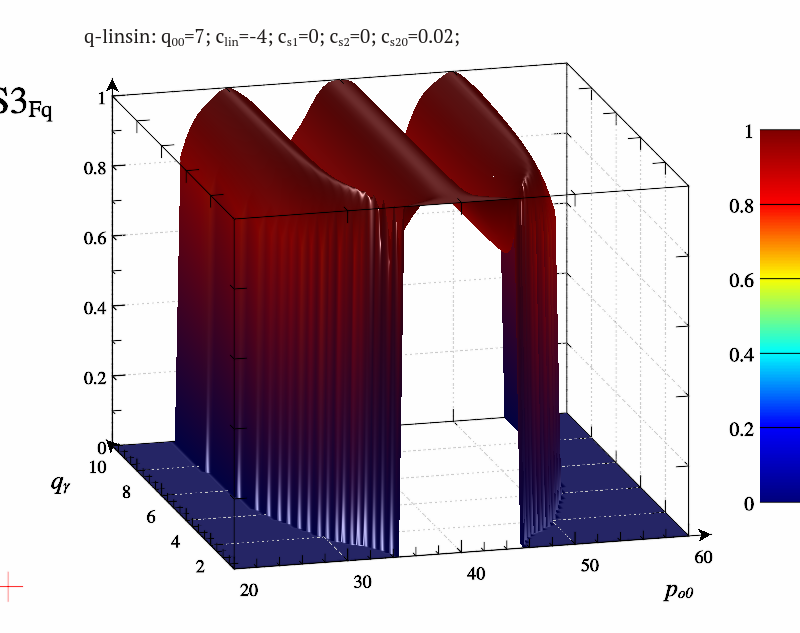
\includegraphics[width=0.32\textwidth]{p/qls_pe-p_po_qg_SFq_s20.png}
    \hfill
    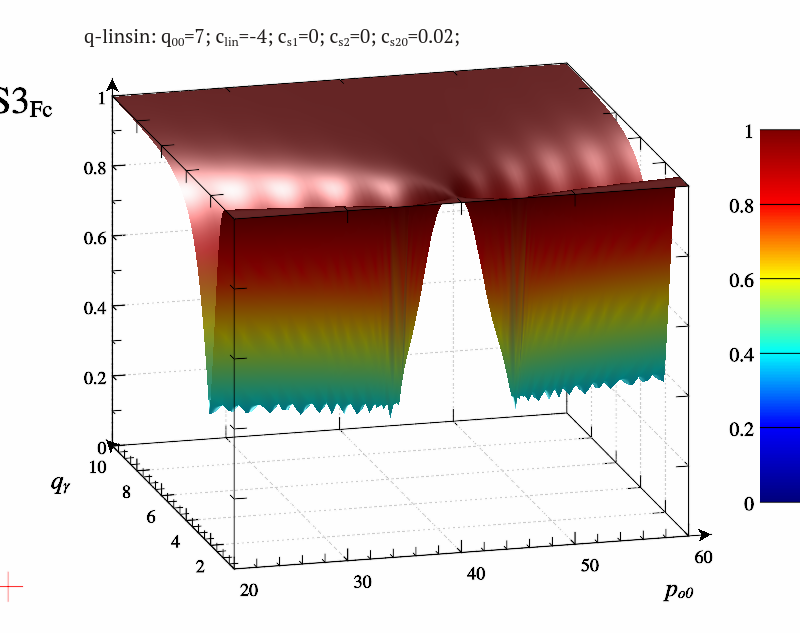
\includegraphics[width=0.32\textwidth]{p/qls_pe-p_po_qg_SFc_s20.png}
  }
  \caption{Зависимости $S(p_o,q_\gamma)$ для методов $p_{eql}$, $p_{eFq}$, $p_{qFc}$ для условий (\ref{atu:eq:q_dem_s20})}
  \label{atu:f:qsl_S_po_qg_s20}
\end{figure}

По сравнению с предыдущим случаем, график для метода $p_{eql}$
имеет ненамного больший охват, при сохранении общей формы.
Это связано с тем, что для данного случая $k_l=1$,
диапазон уверенного определения $p_e$ соответственно расширяется,
что даже избыточно подтверждается невозрастающим уровнем ошибок.
Изменения для метода $p_{qFq}$ не столь заметны,
так как для него не учитывается оценка уровня линейности.
Для метода $p_{eFc}$ сохраняется бессмысленная зависимость.

На рис.~\ref{atu:f:qsl_S_po_qg_lin} представлены те же зависимости зависимости,
но в линейном случае (\ref{atu:eq:q_dem_lin}).

\begin{figure}[htb!]
  \centerline{
    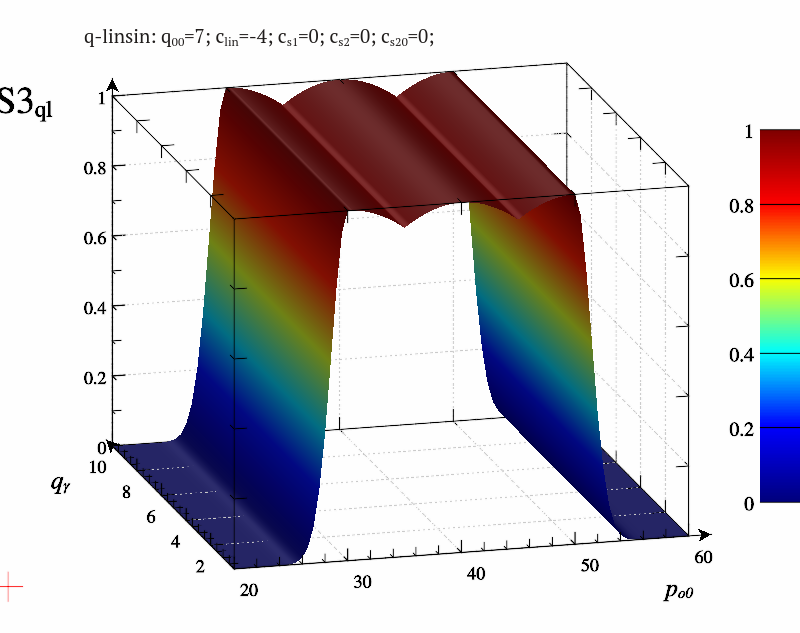
\includegraphics[width=0.32\textwidth]{p/qls_pe-p_po_qg_Sql_lin.png}
    \hfill
    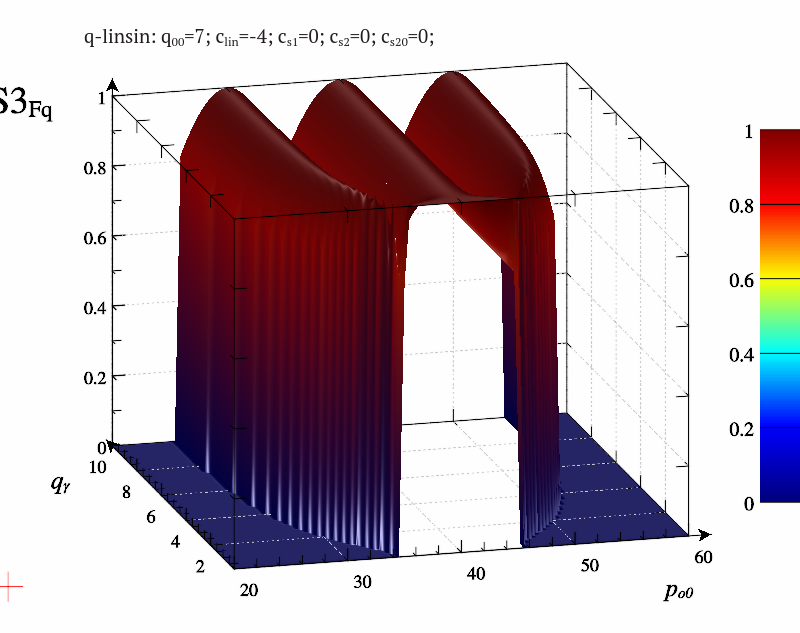
\includegraphics[width=0.32\textwidth]{p/qls_pe-p_po_qg_SFq_lin.png}
    \hfill
    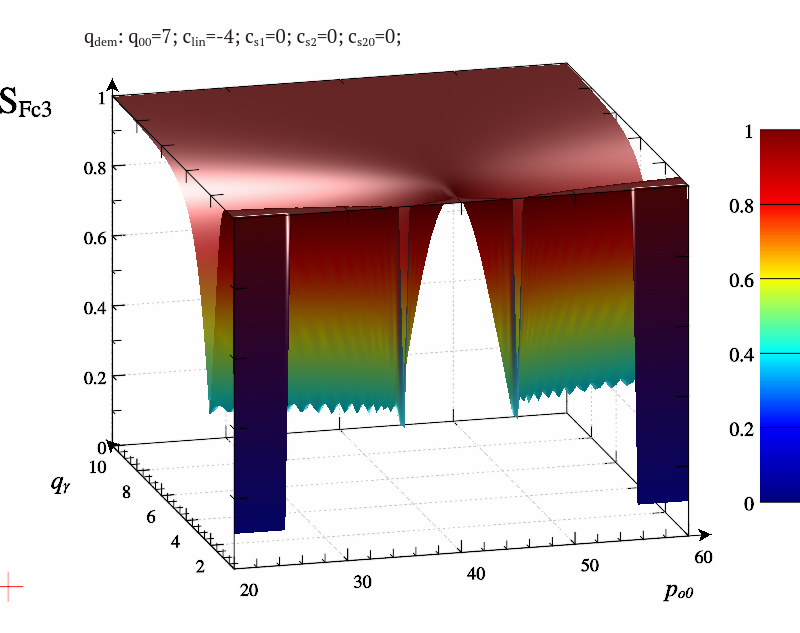
\includegraphics[width=0.32\textwidth]{p/qls_pe-p_po_qg_SFc_lin.png}
  }
  \caption{Зависимости $S(p_o,q_\gamma)$ для методов $p_{eql}$, $p_{eFq}$, $p_{qFc}$ для условий (\ref{atu:eq:q_dem_lin})}
  \label{atu:f:qsl_S_po_qg_lin}
\end{figure}

Принципиальной разницы с предыдущими графиками нет, так отличие
в условиях проявляется на относительно мелком масштабе,
и не влияет на довольно грубую оценку $S$.

На рис.~\ref{atu:f:qsl_W_po_qg_all}, \ref{atu:f:qsl_W_po_qg_s20}, \ref{atu:f:qsl_W_po_qg_lin},
представлены зависимости $W(p_o,q_\gamma)$
для всех рассмотренных вариантов.

\begin{figure}[htb!]
  \centerline{
    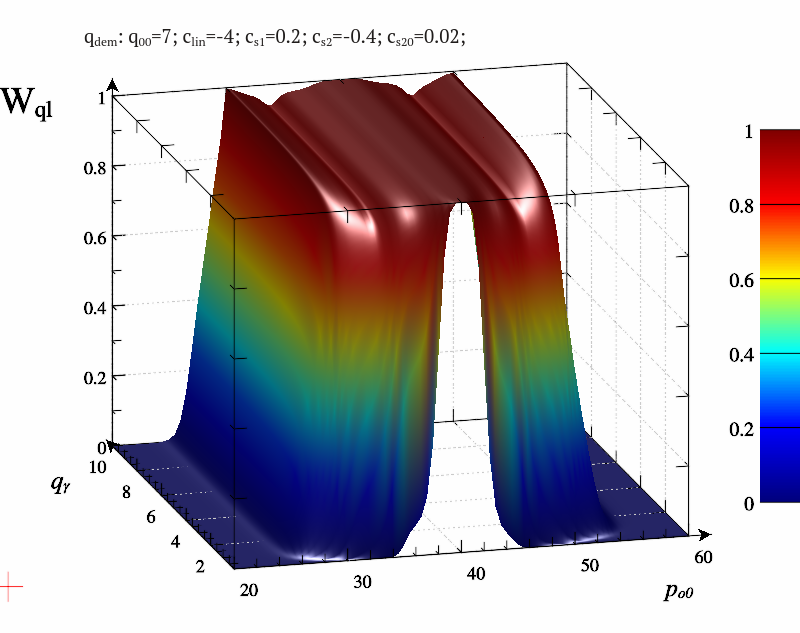
\includegraphics[width=0.32\textwidth]{p/qls_pe-p_po_qg_Wql_all.png}
    \hfill
    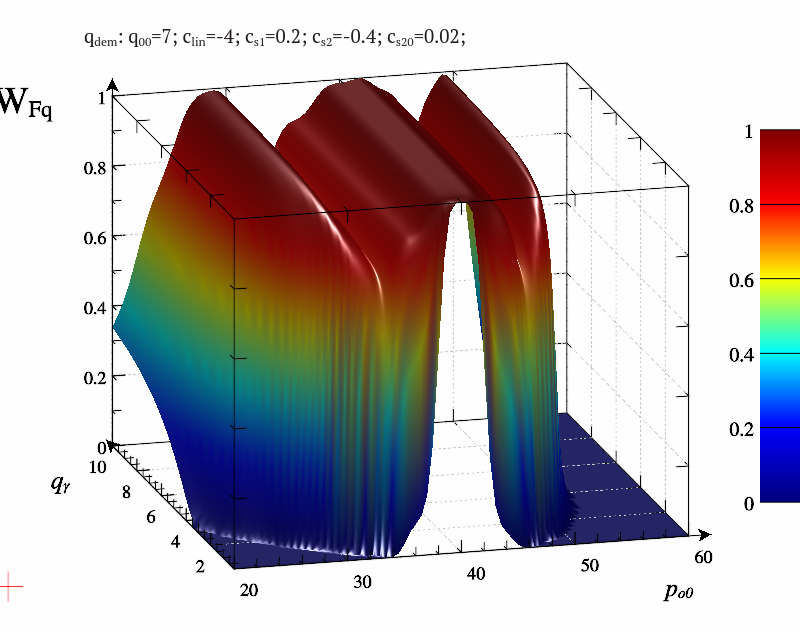
\includegraphics[width=0.32\textwidth]{p/qls_pe-p_po_qg_WFq_all.png}
    \hfill
    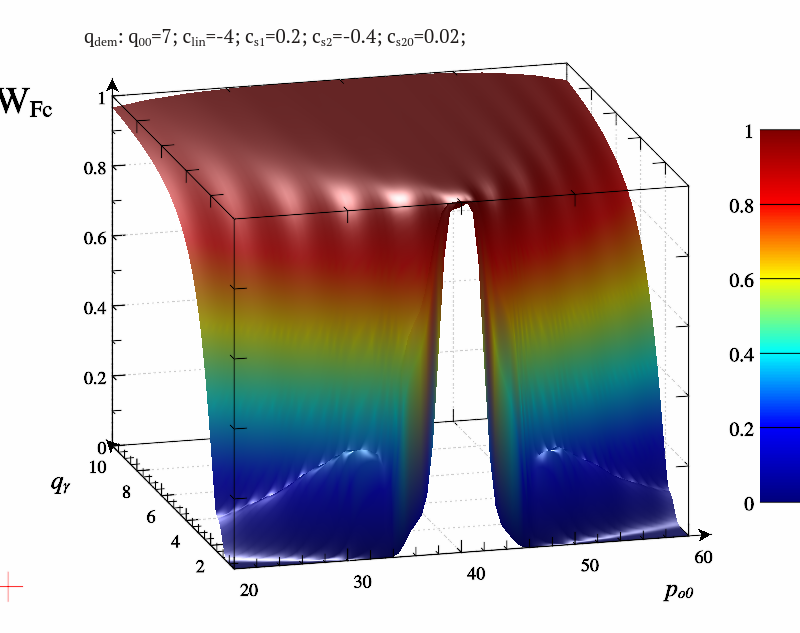
\includegraphics[width=0.32\textwidth]{p/qls_pe-p_po_qg_WFc_all.png}
  }
  \caption{Зависимости $W(p_o,q_\gamma)$ для методов $p_{eql}$, $p_{eFq}$, $p_{qFc}$ для условий (\ref{atu:eq:q_dem_all})}
  \label{atu:f:qsl_W_po_qg_all}
\end{figure}


\begin{figure}[htb!]
  \centerline{
    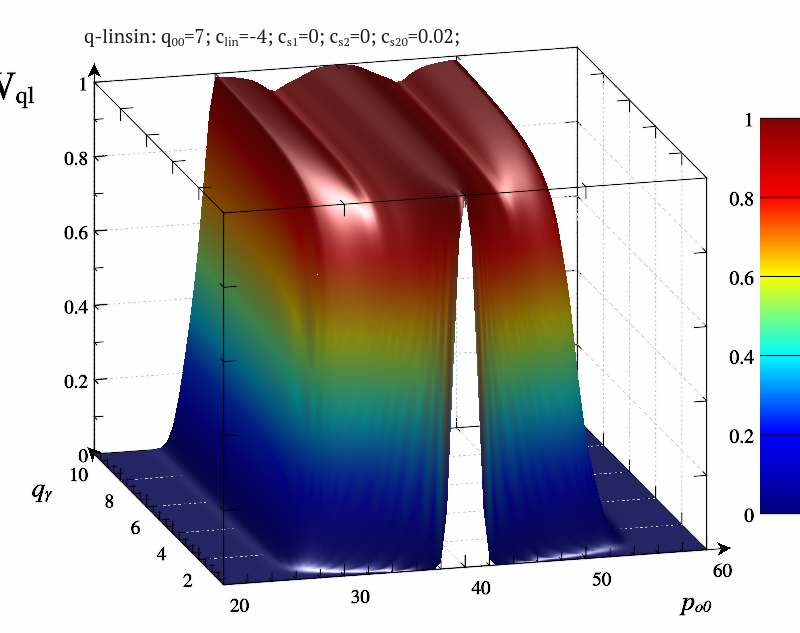
\includegraphics[width=0.32\textwidth]{p/qls_pe-p_po_qg_Wql_s20.png}
    \hfill
    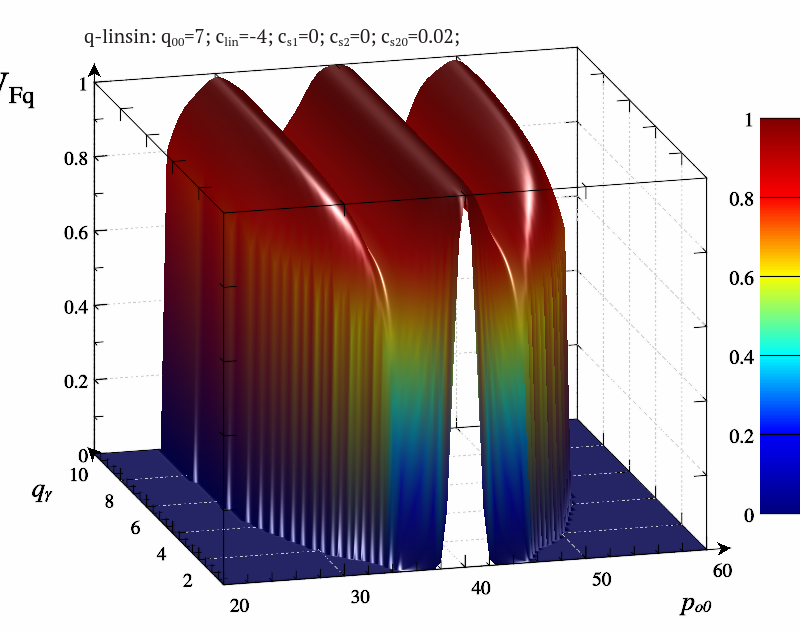
\includegraphics[width=0.32\textwidth]{p/qls_pe-p_po_qg_WFq_s20.png}
    \hfill
    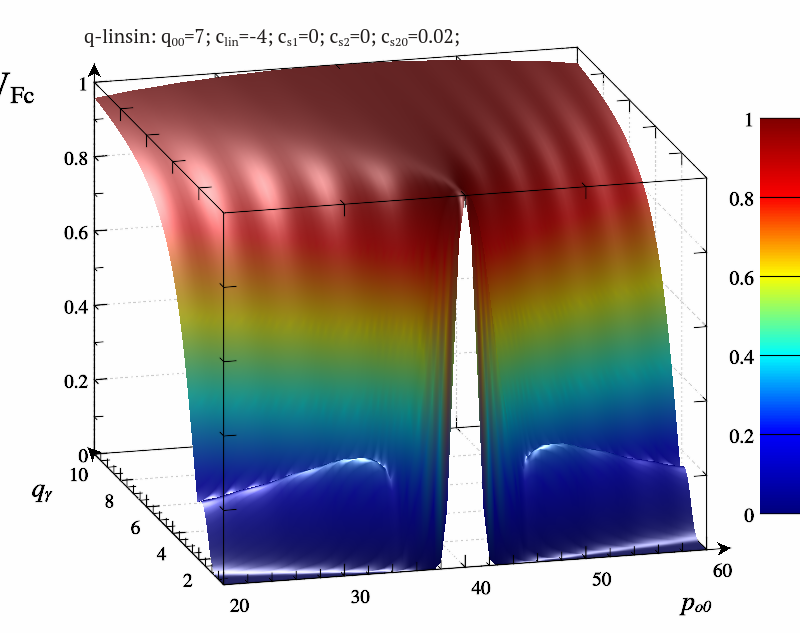
\includegraphics[width=0.32\textwidth]{p/qls_pe-p_po_qg_WFc_s20.png}
  }
  \caption{Зависимости $W(p_o,q_\gamma)$ для методов $p_{eql}$, $p_{eFq}$, $p_{qFc}$ для условий (\ref{atu:eq:q_dem_s20})}
  \label{atu:f:qsl_W_po_qg_s20}
\end{figure}

\begin{figure}[htb!]
  \centerline{
    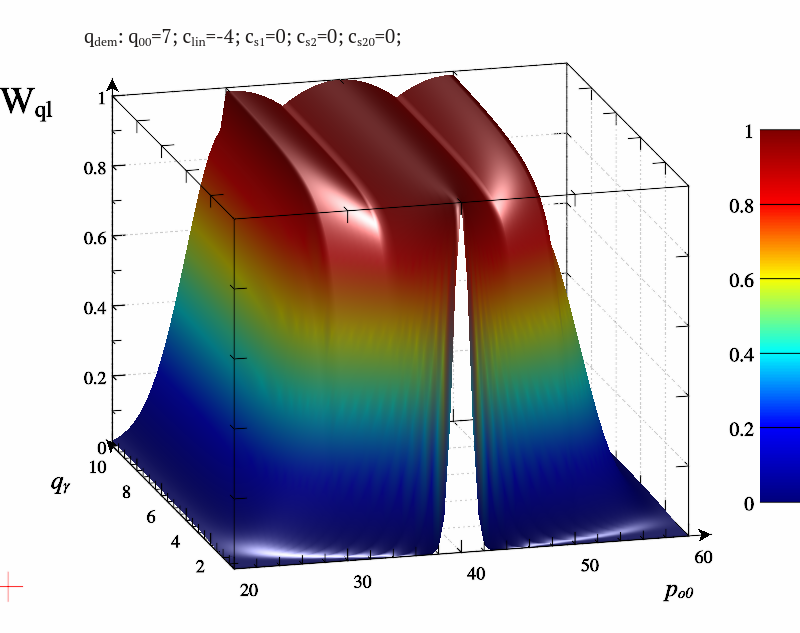
\includegraphics[width=0.32\textwidth]{p/qls_pe-p_po_qg_Wql_lin.png}
    \hfill
    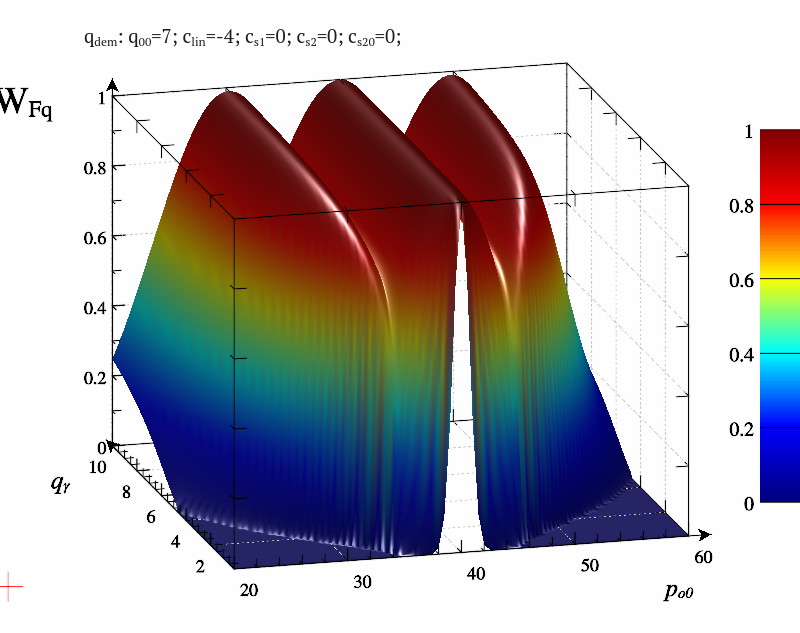
\includegraphics[width=0.32\textwidth]{p/qls_pe-p_po_qg_WFq_lin.png}
    \hfill
    \includegraphics[width=0.32\textwidth]{p/qls_pe-p_po_qg_WFc_lin.png}
  }
  \caption{Зависимости $W(p_o,q_\gamma)$ для методов $p_{eql}$, $p_{eFq}$, $p_{qFc}$ для условий (\ref{atu:eq:q_dem_lin})}
  \label{atu:f:qsl_W_po_qg_lin}
\end{figure}

Наиболее серьезное отличие от зависимостей $S(p_o,q_\gamma)$ наблюдается
для метода $p_{eql}$ --- начинает играть роль ``штраф'' за
избыточную чувствительность функции качества, которая в самом методе
практически не используется. Однако, для рассматриваемой области,
вблизи рабочего диапазона, отличие $W$ от $S$ не имеет особого значения.
Основное предназначение $W$ --- ограничивать динамику агентов,
находящихся вдали от искомого значения~$p_o$.


У другій серії обчислювальних експериментів значення параметра об'єкта було
фіксованим $p_o = 39$, а відстань між агентами $A$ змінювалося від $0.1$
до $20$. При цьому, при $A <1$ точка $p_o$ перебувала за межами інтервалу
$[p_l, p_r]$, і положення $p_e$ визначалося за допомогою екстраполяції.
Значна частина цих графіків відображає протилежний випадок --- $p_O \in [p_l,p_r]$,
і значення $p_e$ визначається інтерполяцією на розширенні (з ростом $A$) діапазоні.

На рис.~\ref{atu:f:qsl_pe_A_qg_all} подані поверхні залежностей помилок ідентифікації
при наявності всіх нелінійних членів.


\begin{figure}[htb!]
  \centerline{
    \includegraphics[width=0.32\textwidth]{p/qls_pe-p_A_qg_eql_all.png}
    \hfill
    \includegraphics[width=0.32\textwidth]{p/qls_pe-p_A_qg_eFq_all.png}
    \hfill
    \includegraphics[width=0.32\textwidth]{p/qls_pe-p_A_qg_eFc_all.png}
  }
  \vspace{-1.5ex}
  \begin{center}
    ~ \hfill a \hfill\hfill b \hfill\hfill c \hfill ~
  \end{center}
  \vspace{-2.5ex}
  \caption{Залежності $e(A,q_\gamma)$ для методов $p_{eql}$ (a), $p_{eFq}$ (b), $p_{qFc}$ (c) при умовах (\ref{atu:eq:q_dem_all})}
  \label{atu:f:qsl_pe_A_qg_all}
\end{figure}

Для методу $p_{eql}$ форма цього графіка досить передбачувана --- немає
залежності від $q_\gamma$, на ділянці екстраполяції величина похибки
лінійно падає при $A \to p_c - p_o$. При подальшому зростанні $A$ похибка
помірно зростає, причому в цьому зростанні можна виділити дві ділянки. Перша
характеризується відносно різким зростанням похибки, що пов'язано зі збільшенням
впливу високочастотних нелінійних членів, друга --- досить плавним підйомом.

Графік, відповідний методу $p_{eFq}$ виявляє явну залежність похибки від
$q_\gamma$. Для широкого діапазону величини $ A $ існує досить вузька область
значень $q_\gamma$, при яких похибка мінімальна. Як надмірна, так і
недостатня чутливість функції якості призводить до зростання похибки.

График, соответствующий методу $p_{eFq}$ проявляет явную зависимость
ошибки от $q_\gamma$. Для широкого диапазона величины $A$
существует достаточно узкая область значений $q_\gamma$,
при которых ошибка минимальна. Как избыточная, так и недостаточная чувствительность
функции качества приводит к росту ошибки.
%
К сожалению,
даже для простейших случаев, подобных рассматриваемому,
получение аналитической зависимости этой области затруднено.
Также этот график отличается меньшей ошибкой в режиме экстраполяции,
но в целом этот метод проигрывает предыдущему.

Графік похибки для методу $p_{eFc}$ підкреслює обмежену придатність цього методу.
%
Аналогично предыдущему методу, существует область наиболее благоприятных для
проведения идентификации значений $q_\gamma$. Однако,
уровень ошибки практически не падает при $p_l \to p_o$,
то есть этот метод не выигрывает в точности при концентрации
агентов в окрестности $p_o$.

Графики (рис.~\ref{atu:f:qsl_pe_A_qg_s20}), построенные с использованием
только высокочастотных нелинейных членов,
подтверждают представленные выше предположения
о влиянии нелинейностей различного частотного масштаба
на ошибку идентификации.

\begin{figure}[htb!]
  \centerline{
    \includegraphics[width=0.32\textwidth]{p/qls_pe-p_A_qg_eql_s20.png}
    \hfill
    \includegraphics[width=0.32\textwidth]{p/qls_pe-p_A_qg_eFq_s20.png}
    \hfill
    \includegraphics[width=0.32\textwidth]{p/qls_pe-p_A_qg_eFc_s20.png}
  }
  \caption{Зависимости $e(A,q_\gamma)$ для методов $p_{eql}$, $p_{eFq}$, $p_{qFc}$ для условий (\ref{atu:eq:q_dem_s20})}
  \label{atu:f:qsl_pe_A_qg_s20}
\end{figure}

При этом метод $p_{eql}$ характеризуется практическим отсутствием роста
ошибки как в режиме экстраполяции, так и при значительном росте $A$.
Метод $p_{eFq}$ также характеризуется существенно меньшим ростом
ошибки, за исключением области избыточной чувствительности.
Вид графика для метода $p_{eFc}$ практически не изменился.

В идеальном случае, при линейной зависимости $q_\mathrm{dem}(p)$~(рис.~\ref{atu:f:qsl_pe_A_qg_lin}),
метод $p_{eql}$ демонстрирует идеальные результаты.
Следует отметить, что в данной тестовой задаче отсутствуют
ошибки измерения.
Метод $p_{eFq}$ позволяет достичь пренебрежимо малой, но не нулевой
ошибки везде, за исключением области экстраполяции и завышенной чувствительности.
При этом, уровень ошибок даже в неблагоприятных областях
относительно мал. Напротив, метод $p_{eFc}$,
даже в идеальных условиях продолжает показывать
посредственные результаты.

\begin{figure}[htb!]
  \centerline{
    \includegraphics[width=0.32\textwidth]{p/qls_pe-p_A_qg_eql_lin.png}
    \hfill
    \includegraphics[width=0.32\textwidth]{p/qls_pe-p_A_qg_eFq_lin.png}
    \hfill
    \includegraphics[width=0.32\textwidth]{p/qls_pe-p_A_qg_eFc_lin.png}
  }
  \caption{Зависимости $e(A,q_\gamma)$ для методов $p_{eql}$, $p_{eFq}$, $p_{qFc}$ для условий (\ref{atu:eq:q_dem_lin})}
  \label{atu:f:qsl_pe_A_qg_lin}
\end{figure}

Таким чином, на підставі результатів моделювання можна зробити висновки про
можливість застосування розглянутих методів:


\begin{itemize}

  \item
    Метод $p_{eFc}$ має гранично  обмежену придатність,
    % единственные преимущества --- простота реализации,
    У подальших дослідженнях в даній цей метод застосовуватися не буде.
    % единственные преимущества --- простота реализации,
    % отсутствие особых случаев и естественная ограниченность
    % $p_e$ не компенсируют все недостатки, поэтому в
    % дальнейших исследованиях в данной этот метод применяться не будет.

  \item
    При нормальному функціонуванні метод $p_{eql}$ забезпечує найкращі
    результати. При цьому він складніше в реалізації, вимагає обробки ряду
    особливих випадків.

  \item
    Метод $p_{eFq}$ демонструє результати, які можна
    порівняти з методом $p_{eql}$, при цьому він простіший в реалізації. У тих
    випадках, коли величина критерію самому агенту безпосередньо не відома, цей
    метод, на відміну від методів, заснованих на апроксимації $q (p)$, зберігає
    працездатність. Недоліком є істотна залежність від величини $q_\gamma$.
    %
    однако, даже методы, которые
    не используют функцию качества на уровне агента, все равно
    применяют её на уровне координатора поиска, и задача выбора адекватной величины $q_\gamma$
    всё равно остаётся.

  \item
    Методи $p_{eql}$ і $p_{qFq}$ дозволяють досягти меншої похибки
    ідентифікації при зближенні пошукових агентів до $p_o$, за умови $p_o \in [p_l, p_r]$.
    %
    Следовательно, для повышения точности идентификации необходимо
    или реализовывать поисковую динамику объекта, или же
    наращивать количество неподвижных агентов, что может быть недостижимо в условиях ограниченности
    ресурсов.


\end{itemize}




% }}}2

\subsection{Динамика поисковых агентов}  % {{{2

Значення $p_e$, отримане пошуковим агентом, може використовуватися
безпосередньо і миттєво в якості значення параметрів для керованих моделей
тільки в тому випадку, якщо об'єкт, і отже моделі, не виявляють власної
динаміки, тобто є статичними. Ідентифікація статичних об'єктів не є ціллю
цієї роботи.

При моделировании произвольной нелинейной динамической системы,
а особенно хаотических систем, нет возможности строго
определить допустимую динамику изменения параметров
в процессе идентификации. Более того, существуют
даже линейные системы, для которых малые, но специальным
образом подобранные параметрические воздействия
приводят к неограниченному росту значений, отображающих
состояние системы. Одним из самых известных примеров
такого поведения является параметрический резонанс~\Cmt{ref:Sivuhin1}.
Для систем динамического хаоса более известным явлением является
сигнальная синхронизация систем, однако,
возможность аналогичных параметрических влияний достаточно очевидна.

Тем не менее, если исключить достаточно редкие особые случаи,
можно оценить допустимую динамику изменения параметров.
Прежде всего, в процессе синтеза критерия идентификации
одним из этапов является определение корректного значения $\tau_q$.
Чаще всего, данная величина неявно задаёт и допустимую
скорость изменения параметров моделей в процессе идентификации.

При моделюванні динаміки тіла без урахування обертання в механіці досить задати
всі сили, що діють на це тіло. Аналогічно, визначаючи пошукову динаміку агента
потрібно визначити еквівалент ``сил'', що викликають зсув параметрів моделей,
контрольованих агентом. При цьому задачу визначення динаміки можна спростити,
розділивши ``сили'' на дві групи. До першої входять сили, що призводять до ``руху''.
У другу входять сили опору, і, замість розгляду самих сил, досить
визначити правила динаміки, при цьому можливе використання правил, які не мають
прямого відображення на реальні фізичні системи.
%
Такое разделение позволяет позволяет более простым образом классифицировать
способы задания поисковой динамики.


\subsubsection{Определения сил, используемых при описании динамики поискового агента}  % {{{3

Розглянемо способи визначення основних діючих сил.

$f_e$ ---
``сила тяжіння'' до локальної оцінки $p_e$, забезпечує зміщення
агента в напрямку цієї точки, і, отже, збільшення ``щільності'' агентів в
околі $p_o$. 
``сила притяжения'' к локальной
оценке $p_e$, обеспечивает смещение агента в направлении этой точки,
и, следовательно, увеличению ``плотности'' агентов в окрестностях $p_o$.
%
Рассмотрим возможные способы определения.

Найпростішим, очевидним, з прозорим фізичним змістом є
наступне визначення:
%
\begin{equation}
  f_e(t) = - k_e \left( p_c(t) - p_e(t) \right)  ,
  \label{atu:eq:f_e_lin}
\end{equation}
%
де $k_e$ --- коефіцієнт пропорційності, що відповідає коефіцієнту жорсткості
умовної ``пружини'', що деформується при видаленні $p_c$ від $p_e$. Це
визначення досить універсальне і має сенс при реалізації багатьох пошукових
тактик.
%
Тем не менее,
это определение не лишено недостатков. Прежде всего,
потенциальная яма, образованная силой вида~(\ref{atu:eq:f_e_lin}),
имеет параболическую форму, и если агент находится на дне этой
ямы, малые внешние силы легко выводят агента из центра данной ямы,
что, в свою очередь, может приводить к снижению точности идентификации.

Вышеупомянутого недостатка лишено следующее определение:
%
\begin{equation}
  f_e(t) = - k_e \sign \left( p_c(t) - p_e(t) \right) ,
  \label{atu:eq:f_e_sign}
\end{equation}
%
образующее треугольную потенциальную яму. При этом,
устранение одного недостатка приводит к появлению
нескольких других. Прежде всего, наличие разрыва
этой функции требует принятия специальных мер по обеспечению
вычислительной устойчивости алгоритмов при
численном моделировании. С другой стороны,
постоянное значение этой функции при отдалении
$p_c$ от $p_e$ может привести к снижению скорости поиска.
В первую очередь этому недостатку будут подвержены
методы идентификации с одним агентом.

Промежуточный способ определения рассматриваемой ``силы''
даёт следующее определение:
%
\begin{equation}
  f_e(t)
  = - k_e \cdot
  \begin{cases}
    1 &  p_c(t) - p_e(t)  > p_\mathrm{sat}
    \\
    \frac{p_c(t)-p_e(t)}{p_\mathrm{sat}} & | p_c(t)-p_e(t)| \le p_\mathrm{sat}
    \\
    -1 &  p_c(t) - p_e(t)  < -p_\mathrm{sat}
  \end{cases},
  \label{atu:eq:f_e_sat}
\end{equation}
%
где  $p_\mathrm{sat}$ --- малая по сравнению с областью поиска величина.
Это определение в какой-то мере объединяет преимущества и недостатки
двух предыдущих.  Нет разрыва в нуле, малые внешние возмущения
приводят к достаточно ограниченным смещениям, но
ограниченность этой зависимости, как и предыдущей,
делает неудобным использование этого определения для систем с одним агентом.

Загальним недоліком визначення сили $f_e$ за виразом (\ref{atu:eq:f_e_lin})
є той факт, що сила визначається тільки по локальним параметрами в околі
агента. Більш того, ігнорується навіть локальне значення впевненості агента в
оцінці $p_e$.
%
Для агентов, находящихся в непосредственной близости к
$p_o$, такое определение силы оправданно. Все остальные агенты
в случае правильного определения направления, будут этой силой прижиматься
к краю своей полосы, если она есть, или же проявлять тенденцию
к сильному скучиванию в противном случае. Более того,
для агентов, находящихся вдали от искомого значения, влияние ошибок измерения
приводит к постоянной смене оценки направления к $p_o$, и как
следствие --- к сильному ``рысканью'' таких агентов.
Следовательно, необходимо ограничение этой силы,
на основании локальных, глобальных, или же и тех и других оценок.
Например:
%
\begin{equation}
  f_e(t) = - k_e S(t) \left( p_c(t) - p_e(t) \right) ,
  \label{atu:eq:f_e_lin_S}
\end{equation}
%
\begin{equation}
  f_e(t) = - k_e F_c(t) \left( p_c(t) - p_e(t) \right) ,
  \label{atu:eq:f_e_lin_F}
\end{equation}
%
\begin{equation}
  f_e(t) = - k_e W(t) \left( p_c(t) - p_e(t) \right) ,
  \label{atu:eq:f_e_lin_W}
\end{equation}

% \Cmt{примеры}

Наявність тільки сили $f_e$ призводить до того, що поведінка агентів буде
практично незалежною, і для реалізації властивостей ``ансамблю'' агентів
необхідне введення сил, що регламентують колективну поведінку. В першу чергу,
слід визначити силу $f_n$, яка визначає взаємодію агента з найближчими
сусідами. У досить загальному випадку цю силу можна визначити як
%
\begin{equation}
  f_n( p_r, p_c, p_l ) = f_{nr}(p_r-p_c) + f_{nl}(p_c-p_l).
  \label{atu:eq:f_n_gen}
\end{equation}

У разі лінійності і однакових визначень функцій $f_{nr}$ і $f_{nl}$ ця залежність набуває вигляду
%
\begin{equation}
  f_n = k_n ( p_r - 2 p_c + p_l ),
  \label{atu:eq:f_n_lin}
\end{equation}
%
де $k_n$ --- масштабний коефіцієнт, що відповідає коефіцієнту жорсткості
``пружин'', що з'єднують агентів. При цьому слід зазначити, що ця функція буде
приймати нульові значення при будь-якому рівномірному розподілі агентів.
%
И, соответственно, будет
противодействовать влиянием, приводящим
к неравномерному распределению.
При этом нет понятия ``естественного расстояния''
между объектами, на котором они находятся в состоянии
устойчивого равновесия при $f_e = 0$.

масштабный коэффициент, соответствующий
коэффициенту жёсткости ``пружин'', соединяющих агенты.

При определённых соотношениях между $k_e$ и $k_n$
возможна ситуация, когда траектории двух агентов пересекаются.
Для некоторых типов агентов, например $p_{eFc}$
это не представляет проблемы. Для большинства других
наличие таких пересечений представляет собой случай,
когда метода определения $p_e$ даёт принципиально
неверные, в том числе неопределённые результаты.
Одним из способов недопущения подобных состояний
является назначение агентам рабочих диапазонов, которые не пересекаются.
%
Другим --- використання нелінійної функции $f_n$,
яка забезпечую сильне, навіть нескісченне відталкування
агентів при сближенні, наприиклад:
%
\begin{equation}
  f_n = k_n \left( \log\left( \frac{p_r-p_c}{p_{d0}} \right) -  \log\left( \frac{p_c-p_l}{p_{d0}}\right) \right),
  \label{atu:eq:f_n_log}
\end{equation}
%
де
$p_{d0}$ ---
базова відстань між агентами, що зазвичай дорівнює початкової відстані:
$p_{d0} = \frac{\Delta p}{N-1}$.




Наличие функции $f_n$ обеспечивает определённые аспекты
коллективного поведения агентов, противодействуя неоправданной
скученности агентов. Том не менее, наличие этой функции во многих задачах
недостаточно для построения работоспособной системы идентификации.
В первую очередь, базовый вид этой функции не препятствует равномерному
сжатию или растяжению, противодействие вызывает лишь неравномерность этих процессов.
Более того, ``пилообразная'' зависимость параметра объекта от времени
может приводить к ситуации, когда  значение параметра агента будут
отслеживать последовательно разные агенты, и как следствие,
весь ансамбль агентов будет
последовательно смещаться в одну сторону.
Таким образом, требуется как минимум ещё одна сила,
которая будет препятствовать таким нежелательным эффектам.
%
Має сенс використовувати $f_c$ --- ``силу тяжіння'' до початкового значення параметра
($p_{c}(0)$) для даної моделі. У лінійній постановці ця сила визначається як
%
\begin{equation}
  f_c = -k_c (p_c - p_{c}(0)) ,
  \label{atu:eq:f_c}
\end{equation}
%
де $k_c$ --- коефіцієнт, що відповідає жорсткості ``пружини'',
що зв'язує агента з його початковим положенням.
Добре зарекомендували себе як нелінійні ``бар'єри'',
так і алгоритмічні методи, які утримують агента
більш-менш жорстко у виділеному йому діапазоні параметра.

Наличие сил $f_n$ и $f_c$ не даёт всем моделям принять одно
и то же значение параметра вблизи экстремума, и, следовательно,
прекратить процесс поиска. Это также позволяет быстро переключиться
на другую модель в случае быстрого изменения параметра объекта.

Результаты моделирования показали, что в большинстве случаев
имеет смысл введение дополнительных сил ``барьерного'' вида,
для исключения пересечения траекторий поисковых агентов,
или же их ухода из рабочего диапазона.

Системы идентификации с одним агентом не требуют описания
динамики коллективного поведения, и для
них силы $f_n$ и $f_c$ разумно считать нулевыми.
Тем не менее, в этом случае постановка задачи может потребовать
ограничения значений параметра модели. Этого можно достичь
как введением дополнительных функций ``барьерного''
вида на границе, так и алгоритмическими ограничениями.

% TODO: searching force
Зважаючи на вищезазначене, визначимо суму всіх ``сил'',
що діють на пошуковий агент:
\begin{equation}
  f_t = f_c + f_n + f_e .
  \label{atu:eq:f_t}
\end{equation}



% }}}3



\subsubsection{Способи визначення пошукової динаміки агента при заданій силі}  % {{{3

\paragraph{Метод ``важкої кульки''}

В этом случае поисковая динамка задаётся следующим образом:%~\Cmt{ref}:
%
\begin{equation}
  m \ddot{p}_c + \nu \dot{p}_c = f_t(t),
  \label{atu:eq:heavy_ball}
\end{equation}
%
де $m$ --- еквівалент маси кульки, $\nu$ --- коефіцієнт умовної в'язкості.
%
Применение этого подхода оправданно,
в первую очередь, при использовании системы идентификации с одним поисковым агентом.
В этом случае ослабляются требования на монотонность зависимости $q(p)$,
или же одноэкстремальности $F(p)$.
К недостаткам данного подхода следует отнести
большие вычислительные затраты,
и повышенные требования к устойчивости поиска.


\paragraph{Метод ``динаміки тіла у в'язкій рідині''}

Також може використовуватися наближення динаміки тіла у в'язкій рідині, коли
вплив інерції дуже малий в порівнянні з в'язкістю, при цьому зміни параметрів
моделей (пошукових агентів) задаються наступним чином:
%
\begin{equation}
  \od{p_c}{t} = v_f f_t(t),
  \label{atu:eq:v_f}
\end{equation}
%
\noindent
де $f_t$ --- сума всіх діючих ``сил'',
$v_f = 1 / \nu$ --- коефіцієнт
пропорційності. Даний підхід, в порівнянні з попереднім, вимагає менших
обчислювальних витрат, і проявляє більшу стійкість. Більш слабкі пошукові
здібності компенсуються застосуванням множини агентів. Тому, в подальшому
викладі для багатомодельних систем буде застосовуватись саме цей підхід.

\paragraph{Специальные подходы}

Существуют методы адаптивно-поисковой идентификации,
определяющие свои правила описания поисковой динамики.
При этом, могут не вводится понятия $p_e$, $f_t$  и другие.
Тем не менее, в целом, эти специальные способы определения динамики
можно свести к используемой терминологии.

Так, например, оригинальный адаптивно-поисковый метод %~\Cmt{ref}
использует поисковые колебания и для определения скорости смещения,
и для реализации смещения как такового. При этом,
после усреднения на интервале поискового периода,
динамика поиска может быть описана выражением~(\ref{atu:eq:v_f}).

Метод с двумя моделями и двумя УГПК~\Cmt{ref}
также задаёт поисковую динамику
специальным образом. В отличие от предыдущего случая,
для определения скорости смещения параметров используется пара
моделей, и смещение реализуется за счёт разности срабатывания двух УГПК.
Тем не менее, и это случае, после усреднения, динамика
может быть описана выражением~(\ref{atu:eq:v_f}).



% }}}3


% }}}2






% }}}1

\section{Методы, параметры и алгоритмы работы поисковых координаторов}  % {{{1

\subsection{Методы определения значения идентифицируемого параметра координатором поиска} % {{{2


Розглянемо набір підходів визначення пошуковим координатором точки максимуму
функції якості, а отже --- значення ідентифікованого
параметра~\cite{atu_st99,atu_jacs2015,atu_st103}.


З усього списку вихідних сигналів пошукових агентів координатор використовує
тільки необхідну йому підмножину.
%
В любом случае, ему необходимы координаты агентов в пространстве параметров, а также величины,
определяющие уровень важности данных данного агента для определения $p_\mathrm{id}$.
%
У якості координати може використовуватися як $p_c$, так і $p_e$.
У якості рівня важливості може використовуватися $F$, $S$, $W$.
%
Возможны и более сложные методы, использующие большее
количество выходных сигналов агента.

В якості першого наближення $p_\mathrm{id}$ можна  використовувати
значення $p_c$ тієї моделі, для якої функція якості максимальна:
%
\begin{equation}
  p_{bcF}
  =
  p_{c,i};
  \quad
  i : F_i = \max{F_j}, \, j=0 \ldots N-1 .
  \label{atu:eq:p_bcF}
\end{equation}

Аналогічно визначаються залежності
$p_{bcS}$ та $p_{bcW}$.
%
Применение величины $p_{bcS}$ представляется достаточно сомнительным,
так как величина $S$ определяется каждым агентом только на основании
локальных данных, и агенты могут быть полностью ``уверенны''
в своей оценке $p_o$, даже в том случае, если они находятся
достаточно далеко от этого значения $F \approx 0$,
но за счёт помех измерения получившие вполне правдоподобную аппроксимацию
$q(p)$ или $F(p)$.

Єдиною перевагою даного методу є простота реалізації. При цьому, ніяк не
використовуються апроксимуючи здатності агентів. Більш того, залежності
$p_{bcA} (t)$ схильні до стрибкоподібих змін в момент перемикання з однієї моделі
на іншу.

Слід зазначити, що для методів, які використовують одну модель, це
практично єдиний метод визначення
$p_\mathrm{id}(t)$.

Для того, щоб використовувати апроксимуючи можливості кожного агента у
визначенні (\ref{atu:eq:p_bcF}) замість $p_c$ можна використовувати $ p_e$.
Відповідні методи отримають позначення $p_{beS}$, $p_{beS} $ і $p_{beW}$.

Для того, щоб використовувати апроксимуючи можливості кожного агента у
визначенні (\ref{atu:eq:p_bcF}) замість $p_c$ можна використовувати $ p_e$.
Відповідні методи отримають позначення $p_{beS}$, $p_{beS} $ і $p_{beW}$.
Такі визначення, на відміну від (\ref{atu:eq:p_bcF}), дозволяють,
при досить хорошій апроксимації $q(p)$ принаймні одним кращим агентом,
реалізувати ідентифікацію для будь-якого
$p_o \in [p_{\min}, p_{\max}]$ при нерухомих агентах.
%
Естественно, при этом точность идентификации будет падать,
особенно при выраженной нелинейности $q(p)$, но значения $p_\mathrm{id}$
не будут ограничены ограниченным набором точек~$p_{i,0}$.
При этом следует отметить, что
значение $p_e$
параметра не соответствует ни одной модели,
следовательно,
значение как функции качества $F$,
так и производной от неё величины $W$
для этой точки неизвестно.
Для тех методов оценки $p_e$, которые позволяют аппроксимировать
значение $F_e$, надёжность этой оценки может быть сомнительна.
Тем не менее, ошибки, возникающие при такой замене,
должны минимизироваться в процессе поиска при $p_{e,i} \to p_o$.


Наступний метод --- реалізація методу COG (Center of gravity, Такагі-Сугено) \cite{atu_asau25,atu_csit2015,atu_asau16},
який використовується при дефазифікації систем нечіткої логіки для всього
ансамблю:
%
\begin{equation}
  p_{gcF}
  =
  \frac{\sum\limits_{i=0}^{N-1} F_{i} p_{i}}
       {\sum\limits_{i=0}^{N-1} F_{i} }
  .
  \label{atu:eq:p_gcF}
\end{equation}

Аналогічно визначаються методи
$p_{gcS}$,
$p_{gcW}$,
$p_{geF}$,
$p_{geS}$ та
$p_{geW}$.


Наступний підхід має призначення зменшити залежність першого від впливу локальних
екстремумів і границь. В цьому випадку визначається модель $M_{i_{m}}$ ($M_{c}$) з
максимальним значенням $F$, а в оцінці використовується тільки найближчий
окіл цієї моделі:
%
\begin{equation}
  p_{lcF}
  =
  \frac{ F_{i-1} p_{c,i-1} + F_{i} p_{c,i} + F_{i+1} p_{c,i+1} }
       { F_{i-1}           + F_{i}         + F_{i+1}         }
  ;
  \quad
  i : F_i = \max{F_j}, \, j=0 \ldots N-1 .
  \label{atu:eq:p_lcF}
\end{equation}
%
или, с учётом введённых локальных обозначений при $i=c$:
%
\begin{equation}
  p_{leF}
  =
  \frac{ F_{l} p_{l} + F_{c} p_{c} + F_{r} p_{r} }
       { F_{l}       + F_{c}       + F_{r}       }
  .
  \label{atu:eq:p_lcFl}
\end{equation}

Аналогічно визначаються методи
$p_{lcS}$,
$p_{lcW}$,
$p_{leF}$,
$p_{leS}$ та
$p_{leW}$.

Так само в околі кращого агента можна використовувати інтерполяцію по
$F$, аналогічно (\ref{atu:eq:p_eFq}). В позначенні таких методів будемо
використовувати перший символ ``q'', наприклад $p_{qeF}$.


Похибки ідентифікації в просторі параметрів для розглянутих підходів позначимо відповідно:
%
\begin{equation}
  e_{gcF} = p_{gcF} - p_o,
  \quad
  e_{leF} = p_{leF} - p_o,
  \quad
  \ldots
  \quad
  e_{leW} = p_{leW} - p_o.
  \label{atu:eq:e_xx}
\end{equation}
%
Если нет необходимости указывать конкретно $F$, $S$ или $W$,
то последний символ в индексе будем опускать.



% }}}2


% }}}1


\section{Классификация и обозначения систем идентификации}  % {{{1
\label{atu:id_classification}

У даній роботі розглядається набір методів ідентифікації нелінійних динамічних
систем. При цьому, більшість з них мають загальні властивості, і система
ідентифікації в цілому складається з ``набору'' модулів і алгоритмів,
комбінація яких дозволяє вибрати конкретний метод, що підходить для даної
задачі.
%
Следовательно, возникает вопрос корректного и непротиворечивого обозначения
используемого метода. Ввиду значительного количества методов, полученных
путём комбинации их элементов, не имеет смысла давать каждому
отдельное названия. Возникает потребность в унификации обозначений
методов, и соответственно, введения определённой классификации.
Часть классификации уже использовалась при
определении методов работы агентов и поисковых координаторов.

Пропонується до використання наступна система позначень, яка послідовно визначає
компоненти системи ідентифікації, починаючи з агентів.

\begin{enumerate}

  \item
  Перший символ (``F'', ``q'', ``x'' ) визначає,
  яка величина використовується кожним агентом для визначення $p_e$.
  %
   Для обозначения методов, для которых в качестве критерия используется
   непосредственно выходы моделей и объектов, будет использоваться символ ``x''.
   При необходимости, при появлении новых подходов,
   могут быть назначены дополнительные символы.

  \item
    Другий символ (``l'' --- linear, ``q'' --- quadratic \ldots ) 
    задає спосіб визначення величини $p_e$ одним агентом.

    \begin{description}

      \item[l]  --- ``linear'' ---
        используется линейная аппроксимация, возможно кусочно-линейная;

      \item[q]  --- ``quadratic'' ---
        используется аппроксимация второго порядка;

      \item[с] --- ``COG'' ---
        метод ``Center of Gravity'' по окрестности агента;

      \item[i] --- ``implicit'' ---
        в явном виде $p_e$ не задаётся, динамика агента задаётся в неявном виде;

      \item[s] --- ``special'' ---
        способ определения выбран на основании особых априорных сведений о виде зависимости $q(p)$;

    \end{description}

  \item
    Третій символ визначає локальну пошукову геометрію, найчастіше --- кількість
    агентів в в пошуковій групі, наприклад: ``2'' --- пошукова пара, ``3'' --- триплет.
    %
    При применении методов, использующих только один поисковый агент,
    этот элемент классификации указывает количество моделей, управляемых этим агентом.

  \item
    Четвертий символ
    описує поведінку додаткових моделей, які розташовані на границі:
    \begin{description}

      \item[z]  --- ``zero'' ---
        реальная модель не используется, функция качества $F$ для неё считается нулевой;

      \item[r] --- ``real'' ---
        используется реальная модель, но без возможности её смещения;

      \item[а] --- ``approximate'' ---
        значение критерия и функции качества каким-то образом аппроксимируются;

      \item[n] --- ``none'' ---
        дополнительные модели не используются;

    \end{description}

  \item
    П'ятий символ
    позначає обрану залежність для величини $f_e$ (або
    аналогічної величини, якщо $f_e$ безпосередньо не використовується):
    \begin{description}

      \item[c]  --- ``const'' ---
        величина $f_e$ не участвует в описании динамики поискового агента;

      \item[l] --- ``linear'' ---
        величина $f_e$ линейно зависит от $p_e$~(\ref{atu:eq:f_e_lin});

      \item[s] --- ``sign'' ---
        используется зависимость вида~(\ref{atu:eq:f_e_sign});

      \item[u] --- ``saturate'' ---
        используется зависимость вида~(\ref{atu:eq:f_e_sat});

    \end{description}

  \item
    Шостий символ  визначає множник,
    що використовується для величини $f_e$ при визначенні динаміки об'єкта:
    \begin{description}

      \item[o]  --- ``one'' ---
        дополнительный множитель не используется (=1);

      \item[F] ---
        используется значение функции качества;

      \item[S] ---
        используется значение ``уверенности'';

      \item[W] ---
        используется значение ``достоинства''.

    \end{description}

  \item
    Сьомий символ
    вказує, яким чином величина $f_t$ (або її еквівалент) впливає на динаміку агента:
    \begin{description}

      \item[z]  --- ``zero'' ---
        агент неподвижен;

      \item[v] --- ``viscous'' ---
        используется модель вязкого трения~(\ref{atu:eq:v_f});

      \item[b] --- ``ball'' ---
        используется подход ``тяжёлого шарика''~(\ref{atu:eq:heavy_ball});

      \item[s] --- ``special'' ---
        особый вид, задаётся методом непосредственно.

    \end{description}

  \item
    Восьмий символ дозволяє вказати,
    який додатковий пошуковий рух реалізує агент:
    \begin{description}

      \item[n]  --- ``none'' ---
        дополнительное поисковое движение не используется,
        при этом, если не возникает неоднозначности в классификации, данный символ можно упустить;

      \item[t] --- ``triangle'' ---
        используется пилообразное поисковое движение, например, реализуемое с помощью УГПК;

      \item[d] --- ``dual'' ---
        используется поисковое движение, реализуемое, например, парой УГПК;

      \item[s] --- ``sin'' ---
        используется гармоническое поисковое движение, применяемое, например, методом синхронного детектора;

      \item[r] --- ``random'' ---
        используется случайное поисковое движение (различные варианты случайного поиска).

    \end{description}


  \item
     Дев'ятий символ задає спосіб визначення ідентифікованого параметра по всьому ансамблю:
    \begin{description}

      \item[b]  --- ``best'' ---
        выбирается лучший агент без дальнейшей обработки;

      \item[g]  --- ``global COG'' ---
        метод ``Center of Gravity'' по всему ансамблю~(\ref{atu:eq:p_gcF});

      \item[l] --- ``local COG'' ---
        метод ``Center of Gravity'' по окрестности лучшего агента~(\ref{atu:eq:p_lcF});

      \item[q] ---
        интерполяция второго порядка в окрестности лучшего агента~(\ref{atu:eq:p_eFq});


    \end{description}

    В случае, если вместо ансамбля используется 1--2 агента, то для определённости будет
    использован символ ``b''


  \item
     Десятий символ визначає, який з вихідних сигналів пошукового агента використовується:
    \begin{description}

      \item[с]  ---  використовується $p_c$;

      \item[e]  --- використовується $p_e$.

    \end{description}

  \item
    Одинадцятий символ вказує,
    яка величина використовується для визначення ваги кожного агента:
    \begin{description}

      \item[F]  ---
        используется $F_c$;

      \item[S]  ---
        используется $S$, без дополнительного уточнения --- $S_{3}$ (\ref{atu:eq:S3});

      \item[W]  ---
        используется $W$.

    \end{description}


\end{enumerate}

Якщо виникає потреба вказати конкретний вид критерію, то в кінець даного
позначення, через точку, додається позначення критерію.
Для позначення підмножин методів замість позначення елемента використовується символ ``A'' --- ``any''.
%
Этим же символом будем обозначать ситуацию,
когда выбор для данного компонента классификации не имеет смысла.

Дополнительное компоненты добавляются в конец после двоеточия.
При необходимости, дополнительно может быть указана группа символов, обозначающая количество
и расположение активных агентов.
В одномерном случае это или просто число, или символ ``N'', если
конкретное количество несущественно. В двумерном случае
используются варианты ``NxM'' для сеточного расположения агентов,
и ``NpM'  --- для конфигурации ``крест''. В случае большей размерности
пространства параметров можно использовать аналогичные обозначения,
но, при необходимости, с дополнительными индексами, например:
``10x10p5'', ``$\mathrm{N_1 p N_2 x N_3 p N_4}$''.

Приклади позначень:
``Fc3zlovngcW.$q_{x^2}$''
--- метод, агенти якого для оцінювання величини $p_e$ використовують функцію
якості і квадратичну апроксимацію за даними кожних трьох сусідніх агентів, 2
псевдомоделі на границі, залежність $f_e (p_e-p_c)$ --- лінійна, ``в'язка''
динаміка, одиничний коефіцієнт при цій силі, ``global COG'' для результуючого
значення параметра по значенням $p_c$ і $W$, критерій
``$q_{x^2}$''.



%``qAuv7.3r.$q_{dx}$''
``ql3ruWvnAeF''
--- группа методов,
для оценивания величины $p_e$ используется критерий и линейная аппроксимацию на триплетах агентов,
2 настоящие модели на границах,
зависимость $f_e$ от $p_e$ --- с насыщением и множителем $W$, ``вязкая'' динамика,
используются все доступные методы для определения  результирующего значения параметра
по значениям $p_e$ и $F_c$.

``xi1nlostbcA'' --- Оригинальный адаптивно-поисковый метод.

``xl2nlosdlcA'' --- Адаптивно-поисковый метод с двумя моделями и двумя УГПК с общим сбросом
 и непосредственным использованием выходов объекта и моделей.

``Fl2nlosdlcA.$q_{x^2}$'' --- Адаптивно-поисковый метод с двумя моделями и двумя УГПК с общим сбросом,
 использующий функцию качества применительно к критерию $q_{x^2}$.



% }}}1


% ----------------------------------------- ERR -------------------------
\section{Качество идентификации}  % {{{1

Среди множества способов оценивания качества идентификации
можно выделить две группы.
К первой группе относятся те, которые производят оценивание
только на основе критерия идентификации, или,
что в какой-то мере эквивалентно, по функции качества идентификации.
В реальных задачах, когда нет возможности определить реальные значения
параметров объекта, это практически единственный вариант.
При этом подразумевается, что как критерий идентификации, так и
функция качества выбраны корректно.

В процессе синтеза новых критериев и методов идентификации
такой подход, с одной стороны, слишком строг,
с другой --- не даёт проверить корректность полученного результата,
так как в этом случае ни близость критериев модели и объекта,
ни, тем более, близкое к единице значение функции качества не
обозначает работоспособность системы идентификации.
Следовательно, при анализе работоспособности,
которые проводятся как на модельных задачах,
так и на реальных физических объектах в контролируемых
условиях, необходимо использовать методы из второй группы,
основанные на сравнении собственно параметров модели и объекта,
то есть на оценивании параметрической
ошибки идентификации $e(t)=p_o(t)-p_\mathrm{id}(t)$.

В работах~\cite{info_cipkin,straton_inf,atu_phd_thesis,karabut} были предложены информационные методы
оценивания качества идентификации.
Они отличаются универсальностью, и отображают
успешность решения одной из основных задач
идентификации --- получения информации то объектах.
Однако, для построения информационных оценок
требуется значительно больше ресурсов, чем
для проведения собственно идентификации. В некоторых случаях,
например, при получении данных с реального оборудования,
это может быть просто невозможно.



За таких умов,
якість ідентифікації для процесу в цілому задається мірою:
%
\[
  \overline{e} = \mu( p_o(t), p_\mathrm{id}(t) ),
  \quad
  t \in [0;T].
\]

Конкретний вид міри визначається задачею. Якщо в конкретній постановці
важливо знати максимальне відхилення ідентифікованого параметра моделі від
об'єкта, то має сенс вибрати міру $C[0; T]$~\cite{kolmogorov_fun_ana} або ж $ R_{\infty}^n$ для
дискретного представлення:
%
\begin{equation}
  \overline{e_c}(p_o(t),p_\mathrm{id}(t))
  =
  \max \big| p_o(t)-p_\mathrm{id}(t) \big|,
  \quad
  t \in [0;T].
  \label{atu:eq:e_c}
\end{equation}

Більш поширеним є випадок, коли інтерес становить не максимальне значення
$|e(t)|$, а якийсь варіант усереднення цієї величини, наприклад
%
\begin{equation}
  \overline{e_2}(p_o(t),p_\mathrm{id}(t))
  =
  \sqrt{ \frac{1}{T} \int\limits_{0}^{T} \big( p_o(t)-p_\mathrm{id}(t) \big)^2 \, \mathrm{d}t },
  \label{atu:eq:e_2}
\end{equation}
%
або
\begin{equation}
  \overline{e_1}(p_o(t),p_\mathrm{id}(t))
  =
  \frac{1}{T} \int\limits_{0}^{T} \big| p_o(t)-p_\mathrm{id}(t) \big| \, \mathrm{d}t .
  \label{atu:eq:e_1}
\end{equation}
%
Этот подход особенно оправдан в тех случаях, когда
значение параметра объекта претерпевает резкие изменения.
При этом, никакая система идентификации не будет успевать за такими
изменениями, особенно с учётом времени, необходимого для
оценивания критерия. Следовательно, если оценивать в таких условиях
качество идентификации, используя \ref{atu:eq:e_c},
то в качестве результата получим всего лишь величину
скачков параметра, а не какие-либо характеристики процесса идентификации.

В тех, достаточно редких случаях, когда из априорной
информации о системе известно, что $p_o(t) = \mathrm{const}$,
имеет смысл в выражениях~(\ref{atu:eq:e_c})--~(\ref{atu:eq:e_1})
ограничить диапазоны для времени, например $[T-\tau_p,T]$,
где $\tau_p$ --- время, достаточное для измерения
критерия идентификации с требуемой точностью.
Это позволит избежать влияния переходных процессов
идентификации на интегральную оценку ошибки.
В остальных случаях, представляет интерес именно реакция
на изменения параметра, поэтому в данной работе преимущественно будет
использоваться выражение~(\ref{atu:eq:e_2}).



Саме значення як похибки ідентифікації, так і відповідної міри ---
величина розмірна і, в такому вигляді, не придатна для незалежного від
конкретної ситуації оцінювання якості роботи методу. Розглянемо можливі
величини, що дають можливість привести похибку ідентифікації до безрозмірного
вигляду.

В першу чергу, припустимо, що взагалі не проводимо ніякої
ідентифікації, а в якості значення параметра використовуємо або геометричний
центр $p_{00}$ множини $\mathcal{P}$, або, якщо це з небудь-якої причини
відомо, точку з максимальним значенням щільності ймовірності. Тоді позначимо
%
\begin{equation}
  \overline{e}_{00}
  =
  \overline{e}(p_o(t),p_{00})
  \label{atu:eq:e_00}
\end{equation}

Відносні похибки для відповідних абсолютних~(\ref{atu:eq:e_xx})
тоді будуть визначені в такий спосіб:
%
\begin{equation}
  \overline{e}_{rbcF} = \frac{\overline{e}_{bcF}}{\overline{e}_{00}}, \;
  \overline{e}_{rleS} = \frac{\overline{e}_{leS}}{\overline{e}_{00}}, \;
  \overline{e}_{rgeW} = \frac{\overline{e}_{geW}}{\overline{e}_{00}},
  \ldots
  \overline{e}_{rqeF} = \frac{\overline{e}_{qeF}}{\overline{e}_{00}}.
  \label{atu:eq:e_rxx}
\end{equation}

Близькість цих величин до одиниці свідчить про те, що даний метод ідентифікації
в розглянутих умовах марний. Більш того, при серйозних порушеннях в процесі
пошуку, наприклад при втраті стійкості, ці величини можуть і перевищувати
одиницю.

Несмотря на очевидную пользу, такой способ приведения к безразмерному виду ошибок
имеет ряд недостатков. Во-первых,
не учитывается возможная мультиагентная структура системы идентификации,
для которой оценка ~(\ref{atu:eq:e_00}) будет слишком грубой.
С другой стороны,
не учитываются свойства
самой системы. Например, возможна такая ситуация, когда параметр
объекта изменяется настолько быстро (по отношению к времени оценивания критерия),
что любой метод идентификации будет бесполезен.

Для оценивания качества работы системы идентификации с счётом
множества моделей, можно воспользоваться несколькими приёмами.
Первый --- пусть все агенты неподвижны, а в качестве $p_\mathrm{id}(t)$
используется $p_c$ той модели, функция качества для которой
максимальна. В терминах применяемой теминологии полученное таким образом значение
параметра обозначается $p_{bc}(t)$ (``best central point''),
соответствующую ему усреднённую ошибку как $\overline{e}_{bc}$.
При этом безразмерные величины обозначим как
$\overline{e}_{gebm}$, $\overline{e}_{lebm}$,  \ldots.
Близость этих величин к единице, при одновременной малости
$\overline{e}_{r*}$, свидетельствует о том, что передвижения
агентов практически бесполезны, и работоспособность системы идентификации достигается
практически только за счёт переключения между агентами.
Одной из причин такого поведения, при условии отсутствия ошибок
в настройке системы, может быть высокая чувствительность
объекта к \textit{динамике} изменения параметра, например
при параметрическом резонансе.

Аналогичный способ, но с учётом возможностей агентов
к аппроксимации --- $p_\mathrm{id}(t)$ определятся
как $p_e(t)$ для лучшего агента.
Соответствующая величина для обезразмеривания обозначается
$\overline{e}_{be}$.
Отношение $\overline{e}_{bc} / \overline{e}_{be}$
характеризует аппроксимирующую способность агентов.

% TODO: start section: test



% }}}1


\section{Исследование работоспособности и свойств методов на тестовых задачах}  % {{{1

\subsection{Постановка тестовых задач}

Для оцінювання можливостей системи ідентифікації відстежувати як гладкі, так і
стрибкоподібні зміни параметрів, пропонується для кожної тестової системи, якщо
це можливо, проводити моделювання процесів ідентифікації за умовами:
%
\begin{equation}
  p_o(t) = p_0 +  U_{p} \sign \sin( \omega_{p} t ),
  \label{atu:eq:po_t_sign}
\end{equation}
%
%
\begin{equation}
  p_o(t) = p_0 +  U_{p} \sin( \omega_{p} t ).
  \label{atu:eq:po_t_sin}
\end{equation}
%
\begin{equation}
  p_o(t) = p_0 +  U_{p} \frac{t}{T}.
  \label{atu:eq:po_t_ramp}
\end{equation}


При этом, использование зависимости вида~(\ref{atu:eq:po_t_sign})
позволяет определить как реакцию системы на скачкообразные
изменения параметра, так и проверить устойчивость процесса поиска.
Использование зависимости~(\ref{atu:eq:po_t_sin}) позволяет проверить
качество ``сопровождения'' системой идентификации плавно изменяющегося параметра,
и, как правило, в этом случае ошибка идентификации должна быть меньше.
Зависимость~(\ref{atu:eq:po_t_ramp}), благодаря линейной зависимости $p_o(t)$
полезна для определения
равномерности работы метода на различных участках $[p_{\min}, p_{\max}]$,
а также для иллюстрации динамики ансамбля поисковых агентов.



\subsection{Равновесные состояния поисковых агентов на текстовой задаче}  % {{{2

Розглянемо конфігурації рівноважного стану пошукових агентів при застосуванні
різних пошукових тактик з числа розглянутих. Для даного завдання немає
необхідності розглядати поведінку координатора пошуку, тому три правих символу
класифікації тут значення не мають.
Використовувалося 5 пошукових агентів: $A_0 \ldots A_4$, початкові
координати яких ($p_{ci,0}$) були розподілені по пошуковому діапазону
рівномірно. Залежність $p_o (t)$ задана як (\ref{atu:eq:po_t_ramp}), при
цьому величини $p_o$ і $U_p$ обрані таки чином, щоб покрити весь робочий
діапазон: $p_0 = p_{c0,0} = 20$, $U_p = p_{c4,0} - p_{c0,0} = 40$.

Так как в данной задаче исследуются равновесные состояния, то
необходимо обеспечить квазиравновесность системы.
Это было достигнуто за счёт того, что
в значение $q(p)$ не взносилась дополнительная задержка,
а общее время наблюдения $T$ было выбрано заведомо и значительно большим,
чем характерное время переходных процессов.

При анализе равновесных состояний конфигураций $p_{ci}(t)$,
которые в силу квазистационарности и выбранной зависимости $p_o(t)$
эквивалентны конфигурациям $p_{ci}(p_o)$,
в первую очередь обращалось внимание на поведение агентов
вблизи $p_o$: требуется наличие как минимум двух агентов в этой окрестности,
допустимо наличие трёх, наличие большего количества представляется нерациональным.
Следующей важным свойством является отсутствие колебаний,
которые свидетельствовали бы о неустойчивости системы идентификации в целом.
Также рассматривалось поведение дальних по отношению к $p_o$
агентов, так как чрезмерное их смещение может негативно
сказываться на динамических характеристиках метода.

На рис.~\ref{atu:f:qls_ramp_Fq3rlovnAAF} наведені результати моделювання при використанні групи методів
``Fq3rlovnAAF''. Слід зазначити, що практично у всьому діапазоні об'єкт
``супроводжується'' двома агентами, і тільки в області ``передачі'' наступній
групі це число зростає до трьох. Слід зазначити відсутність коливань. До
негативних явищ можна буде віднести те, що віддалені агенти притискаються до
кордону виділеної їм області, що обумовлено використанням одиничного множника у
визначенні $f_e$. Також необхідно відзначити збільшення
``дистанції супроводу'' в околі точки $p_o = 40$, $t = 10$.

\begin{figure}[htb!]
  \centerline{
    \includegraphics[width=0.8\textwidth]{p/ramp/qls-p_t_pi_Fq3rlovnAAF_ramp.png}
  }
  \caption{Равновесные конфигурации агентов при использовании группы методов Fq3rlovnAAF}
  \label{atu:f:qls_ramp_Fq3rlovnAAF}
\end{figure}

На рис.~\ref{atu:f:qls_ramp_Fq3rlFvnAAF} приведены результаты моделирования
при использовании метода Fq3rlFvnAAF.
Основное отличие от предыдущего
случая заключается в использовании коэффициента $S$ в определении $f_e$.
Как результат, самые дальние агенты смещаются на меньшее расстояние.
В то же время, поведение агентов, ``сопровождающих'' $p_o$,
остаётся практически без изменений.


\begin{figure}[htb!]
  \centerline{
    \includegraphics[width=0.8\textwidth]{p/ramp/qls-p_t_pi_Fq3rlFvnAAF_ramp.png}
  }
  \caption{Равновесные конфигурации агентов при использовании метода Fq3rlFvnAAF}
  \label{atu:f:qls_ramp_Fq3rlFvnAAF}
\end{figure}

На рис.~\ref{atu:f:qls_ramp_Fq3rlSvnAAF} приведены результаты моделирования
при использовании метода Fq3rlSvnAAF.
Здесь в качестве множителя при определении силы $f_e$ используется
величина $S$, которая не определяется достаточно корректно
для используемого метода оценки $p_{eFq}$. Как результат,
поведение агентов становится не вполне адекватным.
``Сопровождение'' как таковое осталось, однако,
возросшая дистанция должна привести к увеличению ошибки идентификации.
Поведение остальных агентов, хоть и объяснимо, не способствует
проведению идентификации.

\begin{figure}[htb!]
  \centerline{
    \includegraphics[width=0.8\textwidth]{p/ramp/qls-p_t_pi_Fq3rlSvnAAF_ramp.png}
  }
  \caption{Равновесные конфигурации агентов при использовании метода Fq3rlSvnAAF}
  \label{atu:f:qls_ramp_Fq3rlSvnAAF}
\end{figure}


На рис.~\ref{atu:f:qls_ramp_Fq3rlWvnAAF} приведены результаты моделирования
при использовании метода Fq3rlWvnAAF.
В этом случае в качестве множителя используется величина $W$,
в определении которой используется уже рассмотренная в предыдущем случае величина $S$.
В результате получившаяся картина слабо отличается от предыдущего случая,
хотя определённая ненулевая работоспособность всё-таки присутствует.

\begin{figure}[htb!]
  \centerline{
    \includegraphics[width=0.8\textwidth]{p/ramp/qls-p_t_pi_Fq3rlWvnAAF_ramp.png}
  }
  \caption{Равновесные конфигурации агентов при использовании метода Fq3rlWvnAAF}
  \label{atu:f:qls_ramp_Fq3rlWvnAAF}
\end{figure}

Следующая группа методов отличается от предыдущей тем, что для оценки величины $p_e$
используется метод $p_{eql}$, который показал в целом лучшие результаты
при использовании триплета неподвижных агентов.
На рис.~\ref{atu:f:qls_ramp_ql3rlovnAAF} приведены результаты моделирования
при использовании метода ql3rlovnAAF, который характеризуется
единичным множителем в определении  $f_e$. Основное отличие от
аналогичного метода Fq3rlovnAAF заключается в том, что в окрестности
точки $t=10$ расстояние между ``сопровождающими'' агентами не растёт,
следовательно, не следует ожидать и роста ошибки идентификации в окрестности этой точки.
Поведение ``дальних'' агентов остаётся аналогичным.


\begin{figure}[htb!]
  \centerline{
    \includegraphics[width=0.8\textwidth]{p/ramp/qls-p_t_pi_ql3rlovnAAF_ramp.png}
  }
  \caption{Равновесные конфигурации агентов при использовании метода ql3rlovnAAF}
  \label{atu:f:qls_ramp_ql3rlovnAAF}
\end{figure}

Вполне ожидаемые результаты получены при применении
метода ql3rlFvnAAF, которые иллюстрирует
рис.~\ref{atu:f:qls_ramp_ql3rlFvnAAF}.
Введение коэффициента $F$ приводит к меньшему смещению ``дальних''
агентов, и, потенциально --- к уменьшению
времени переключения при скачкообразном изменении $p_o$.

\begin{figure}[htb!]
  \centerline{
    \includegraphics[width=0.8\textwidth]{p/ramp/qls-p_t_pi_ql3rlFvnAAF_ramp.png}
  }
  \caption{Равновесные конфигурации агентов при использовании метода ql3rlFvnAAF}
  \label{atu:f:qls_ramp_ql3rlFvnAAF}
\end{figure}


Существенное отличие в равновесной конфигурации агентов
наблюдается при переходе от способа оценки $p_e$ от $p_{eFc}$ к $p_{eql}$,
например,
при использовании метода ql3rlSvnAAF
(рис.~\ref{atu:f:qls_ramp_ql3rlSvnAAF}).
Так как в этом случае применяется значительно более корректное определение величины~$S$,
то и распределение агентов потенциально является более благоприятным для
проведения идентификации.

\begin{figure}[htb!]
  \centerline{
    \includegraphics[width=0.8\textwidth]{p/ramp/qls-p_t_pi_ql3rlSvnAAF_ramp.png}
  }
  \caption{Равновесные конфигурации агентов при использовании метода ql3rlSvnAAF}
  \label{atu:f:qls_ramp_ql3rlSvnAAF}
\end{figure}


В этих условиях успользование в качестве множителя величины~$W$
не приводит к кардинальноу изменению поведения агентов
(рис.~\ref{atu:f:qls_ramp_ql3rlWvnAAF}) --- метода ql3rlWvnAAF.
Отличие проявляется в меньшем смещении удалённых
агентов, что, без существенного изменения точности
должно приводить к уменьшеню времени реакции системы на скачкообразное
изменение параметра.


\begin{figure}[htb!]
  \centerline{
    \includegraphics[width=0.8\textwidth]{p/ramp/qls-p_t_pi_ql3rlWvnAAF_ramp.png}
  }
  \caption{Равновесные конфигурации агентов при использовании метода ql3rlWvnAAF}
  \label{atu:f:qls_ramp_ql3rlWvnAAF}
\end{figure}

Таким чином, встановлено, що в тих випадках, коли для оцінювання $p_e$ використовується
метод $p_{eFq}$, то немає сенсу в якості множника при $f_e$
використовувати $S$ або $W$. Найкращим вибором в цих умовах буде
використання значення функції якості~$F$. До того ж, що підтверджується і
результатами дослідження якості апроксимації $q(p)$, використання методів,
які використовують кусково-лінійну апроксимацію, найбільш прийнятно. У цих
умовах стає виправданим в якості вищезгаданого множника використовувати~$S$
і~$W$, причому останній варіант видається більш виправданим.

% }}}2

\subsection{Ошибки идентификации в квазистационарном случае на тестовой задаче}  % {{{2

Рівноважні конфігурації агентів, які були представлені вище, дають інформацію тільки про
потенційні властивості систем ідентифікації.
В першу чергу, якість визначається похибкою ідентифікації.
%
В первую очередь следует исследовать её зависимости для квазистационарного случая.
При этом, следует проверять как достижение самого стационарного режима,
так и зависимость ошибки от $p_o$. Для грубого сравнения достаточно
использовать среднеквадратичное значение ошибки на всём рабочем диапазоне параметра,
визуально контролируя форму зависимости $e(p_o)$.
%
В якості тестової задачі
використовується~(\ref{atu:eq:q_dem}) з усіма нелінійними членами~(\ref{atu:eq:q_dem_all}).
При цьому для кожного методу
проводилася серія обчислювальних експериментів з різним значенням~$p_o$. Інші
параметри як системи ідентифікації, так і умови експериментів вибиралися таким
чином, щоб з одного боку, забезпечити квазістаціонарність в кінці експерименту, а
з іншого --- досягти хорошої швидкості ідентифікації, для надання можливості
досліджувати динамічні властивості без переналаштовування параметрів.

Представлення отриманих результатів ускладнюється тим, що з урахуванням тільки
основних розглянутих елементів в класифікації, виходить 192 можливих метода.
%
Для большей компактности представления результатов
воспользуемся тем фактом, что в рассмотренных методах
координатор поиска не настраивает параметры агентов.
%
Тому на одному графіку можна відобразити залежності для восьми методів.
%
что соответствует полному перебору
двух предпоследних символов в классификации,
которые для обозначения группы методов будут
указаны как ``AA'', а конкретное значение этих символов
будет указано в легенде графика. Например,
кривая, обозначенная как ``$e_{ge}$'' для группы методов
``Fq3rlovnAAW'' будет описывать
ошибку идентификации для метода ``Fq3rlovngeW''.
Таким образом результаты можно представить на 24 графиках,
что также представляется несколько избыточным.

В первую очередь рассмотрим методы, которые давали
недостаточно адекватные результаты при
исследовании равновесных конфигураций агентов, а именно ---
методы, которые для аппроксимации $p_e$
используют метод $p_{qFc}$, и при этом в качестве
множителя в определении $f_e$ используют величины $S$ или $W$.
В качестве примера рассмотрим группу методов ``Fq3rlWvnAAF'',
зависимости $e(p_o)$ для которой приведены на рис.~\ref{atu:f:Fq3rlWvnAAF_scan}.

\begin{figure}[htb!]
  \centerline{
    \includegraphics[width=0.8\textwidth]{p/scan/qls-p_p_e_Fq3rlWvnAAF_scan.png}
  }
  \caption{Зависимости $e(p_o)$ для группы методов Fq3rlWvnAAF в квазистационарном случае}
  \label{atu:f:Fq3rlWvnAAF_scan}
\end{figure}

Анализ полученных зависимостей позволяет сделать следующие выводы.
Во-первых, несмотря на недостаточно адекватные равновесные конфигурации
самих агентов, методы идентификации в целом не потеряли работоспособности.
При этом ни один из методов работы координатора поиска
не даёт заметно выделяющихся результатов.
Лучшие результаты продемонстрировали методы
``Fq3rlWvnqeF'' и ``Fq3rlWvnbeF''.
Аналогичные результаты были получены для все методов групп
``Fq3rlSvnAAA'' и ``Fq3rlWvnAAA'', конкретный ``лучший'' метод
мог меняться, но в целом картина оставалась такой же.

В качестве более удачного примера рассмотрим
группу методов ``Fq3rlFvnAAF'' (рис.~\ref{atu:f:Fq3rlFvnAAF_scan}).

\begin{figure}[htb!]
  \centerline{
    \includegraphics[width=0.8\textwidth]{p/scan/qls-p_p_e_Fq3rlFvnAAF_scan.png}
  }
  \caption{Зависимости $e(p_o)$ для группы методов Fq3rlFvnAAF в квазистационарном случае}
  \label{atu:f:Fq3rlFvnAAF_scan}
\end{figure}

При общем меньшем уровне ошибки идентификации, среди различных подходов
к реализации методов работы поисковых координаторов появились явные лидеры и
выраженные зависимости. Прежде всего, методы, использующие значения $p_e$
каждого агента, показывают меньшую ошибку, по сравнению а аналогичными методами,
но использующие $p_c$. Это свидетельствует о том, что
использование подкреплённых соответствующим измеренным значением $F_c$ величин
хуже, чем использование аппроксимированных значений $p_e$,
для которых соответствующее значение функции качества неизвестно.
Методы, использующие глобальный ``COG'', в целом
дают худшие результаты, чем использующие различные локальные оценки.
Лучшие результаты показали методы
``Fq3rlFvnqeF'' и ``Fq3rlFvnbeF''.

Использование при оценке значимости агента величины $S$ вместо $F$
даёт несколько противоречивые результаты (рис.~\ref{atu:f:Fq3rlFvnAAS_scan}).

\begin{figure}[htb!]
  \centerline{
    \includegraphics[width=0.8\textwidth]{p/scan/qls-p_p_e_Fq3rlFvnAAS_scan.png}
  }
  \caption{Зависимости $e(p_o)$ для группы методов Fq3rlFvnAAS в квазистационарном случае}
  \label{atu:f:Fq3rlFvnAAS_scan}
\end{figure}

Если значимость агента оценивается только по его локальной
``самооценке'', то худшие методы показывают несколько
лучшие результаты, а лучшие --- наоборот, несколько
худшие.
При этом следует помнить, что величина $S$
для методов ``Fq3\ldots'' не имеет достаточно корректного представления.
Группу лидеров составляют методы
``Fq3rlFvnleS'', ``Fq3rlFvnqeS'' и ``Fq3rlFvnbeS''.

Использование при оценке значимости агента величины $W$,
несмотря на то, что её определении участвует уже рассмотренная величина $F$
даёт промежуточные результаты (рис.~\ref{atu:f:Fq3rlFvnAAW_scan}).

\begin{figure}[htb!]
  \centerline{
    \includegraphics[width=0.8\textwidth]{p/scan/qls-p_p_e_Fq3rlFvnAAW_scan.png}
  }
  \caption{Зависимости $e(p_o)$ для группы методов Fq3rlFvnAAW в квазистационарном случае}
  \label{atu:f:Fq3rlFvnAAW_scan}
\end{figure}

Несмотря не несколько худшие результаты, показанные лучшими
методами, в целом все методы этой группы показывают
весьма неплохие результаты. Нет ни значительных прыжков для ``bc'',
ни размаха ``ge''.
В этой группе методов лучшие результаты показывают
``Fq3rlFvnqeS'' и ``Fq3rlFvnbeS''.


Рассмотрим, какие изменения произойдут, если использовать
единичный множитель в определении $f_e$ на примере группы методов ``Fq3rlovnAAW''
(рис.~\ref{atu:f:Fq3rlovnAAW_scan}).

\begin{figure}[htb!]
  \centerline{
    \includegraphics[width=0.8\textwidth]{p/scan/qls-p_p_e_Fq3rlovnAAW_scan.png}
  }
  \caption{Зависимости $e(p_o)$ для группы методов Fq3rlovnAAW в квазистационарном случае}
  \label{atu:f:Fq3rlovnAAW_scan}
\end{figure}

Несмотря на заметную разницу в равновесной конфигурации агентов
для методов ``Fq3rlFvnAAW'' и ``Fq3rlovnAAW'',
разница в ошибке идентификации практически не заметна.
Это связано с тем, что агенты, положение которых изменилось,
вносят несущественный вклад в полученное значение $p_\mathrm{id}$.
Однако, это справедливо только для квазистационарного случая.
Тем не менее, это даёт возможность сократить количество методов для
анализа на данном этапе.

Сводные результаты среднеквадратичных ошибок идентификации, для методов ``Fq3r\ldots''
приведены в таблице~\ref{atu:t:err_test_id_Fq}.

\begin{table}[htb!]
  \caption{Ошибки идентификации в квазистационарном случае при аппроксимации $p_e$ методом $p_{eFq}$}
  \label{atu:t:err_test_id_Fq}
  \begin{center}
    \begin{tabular}{|l|c|c|c|c|c|c|c|c|}
    \hline
    Method      & gc    & lc    & qc    & bc    & ge     & le    & qe    & be    \\ \hline
    Fq3rlovnAAF & 2.020 & 0.778 & 0.135 & 0.332 & 0.750  & 0.547 & 0.135 & 0.135 \\ \hline
    Fq3rlovnAAS & 0.733 & 0.797 & 0.959 & 1.033 & 0.385  & 0.319 & 0.321 & 0.318 \\ \hline
    Fq3rlovnAAW & 0.679 & 0.554 & 0.530 & 0.521 & 0.364  & 0.296 & 0.247 & 0.245 \\ \hline
    Fq3rlFvnAAF & 1.980 & 0.778 & 0.136 & 0.334 & 0.761  & 0.546 & 0.136 & 0.136 \\ \hline
    Fq3rlFvnAAS & 0.734 & 0.798 & 0.960 & 1.036 & 0.386  & 0.321 & 0.323 & 0.320 \\ \hline
    Fq3rlFvnAAW & 0.680 & 0.555 & 0.530 & 0.524 & 0.366  & 0.297 & 0.249 & 0.247 \\ \hline
    Fq3rlSvnAAF & 2.520 & 2.082 & 1.180 & 1.352 & 1.569  & 1.575 & 1.160 & 1.164 \\ \hline
    Fq3rlSvnAAS & 1.585 & 1.521 & 1.441 & 2.077 & 1.248  & 1.164 & 1.203 & 1.204 \\ \hline
    Fq3rlSvnAAW & 1.540 & 1.322 & 0.985 & 1.390 & 1.233  & 1.152 & 1.156 & 1.162 \\ \hline
    Fq3rlWvnAAF & 2.541 & 2.092 & 1.208 & 1.368 & 1.568  & 1.573 & 1.187 & 1.192 \\ \hline
    Fq3rlWvnAAS & 1.608 & 1.548 & 1.458 & 2.095 & 1.272  & 1.189 & 1.230 & 1.232 \\ \hline
    Fq3rlWvnAAW & 1.562 & 1.355 & 1.002 & 1.406 & 1.259  & 1.180 & 1.184 & 1.191 \\ \hline
    \end{tabular}
  \end{center}
\end{table}

Нижняя половина этой таблицы соответствует методам,
которые показали свою ограниченную пригодность, и в дальнейшем
рассматриваться не будут, по крайней мере до тих пор,
пока для них не появится достаточно корректное определение величины $S$.
Верхней половина таблицы позволяет обобщить выводы о том, что
глобальные методы координаторов показывают худшие результаты, чем локальные,
использование $p_e$ предпочтительнее $p_c$,
и лучшие результаты демонстрируют методы ``\ldots qeA''  и ``\ldots beA''.

Рассмотрим аналогичные зависимости для методов, агенты в которых
используют для аппроксимации $p_e$ метод $p_{eql}$.
Для этих методов, в отличие от рассмотренных выше,
есть возможность корректного определения величин $S$ и $W$.
Следовательно, нет необходимости убирать часть методов из числа рассматриваемых.

Начнём анализ с группы методов ``ql3rlFvnAAF''~(рис.~\ref{atu:f:ql3rlFvnAAF_scan}), для упрощения сравнения
с ранее описанными методами, для которых первым рассмотренным нормально работающим был ``Fq3rlFvnAAF''.
Рассмотрим применение единичного множителя в определении $f_e$ на примере группы методов ``Fq3rlovnAAW''.

\begin{figure}[htb!]
  \centerline{
    \includegraphics[width=0.8\textwidth]{p/scan/qls-p_p_e_ql3rlFvnAAF_scan.png}
  }
  \caption{Зависимости $e(p_o)$ для группы методов ql3rlFvnAAF в квазистационарном случае}
  \label{atu:f:ql3rlFvnAAF_scan}
\end{figure}

В представленных зависимостях, про сравнению с методами ``Fq3\ldots'', наблюдаются
как общие характеристики, так и новые свойства. В первую очередь,
использование метода координатора ``ge'' даёт худшие результаты,
и наблюдается аналогичная форма зависимости.
Совершенно аналогично, методы с использованием величин $p_e$ агентов
дают лучшие оезультаты, чем методы,  использующие $p_c$.
Также близок к аналогичному набор лучших метдов из группы:
``ql3rlFvnleF'', ``ql3rlFvnqeF'' и ``ql3rlFvnbeF''.
Значительным отличием является существенно меньший уровень ошибки
идентификации для этих методов, при этом разница между
``le'', ``qe'' и ``be'' пренебрежимо мала.


Использование при этих же условиях на уровне координатора поиска
величины $S$ (группа методов ``ql3rlFvnAAS'', рис.~\ref{atu:f:ql3rlFvnAAS_scan}) заметно
изменяет картину только для ``глобальных'' методов,
причём немного и в лучшую сторону.
Из списка лучших выпал метод, использующий ``le'',
для двух оставшихся изменение ошибки пренебрежительно мало.
Из негативных явлений стоит отметить увеличение скачкообразных
изменений ошибки для некоторых из методов.

\begin{figure}[htb!]
  \centerline{
    \includegraphics[width=0.8\textwidth]{p/scan/qls-p_p_e_ql3rlFvnAAS_scan.png}
  }
  \caption{Зависимости $e(p_o)$ для группы методов ql3rlFvnAAS в квазистационарном случае}
  \label{atu:f:ql3rlFvnAAS_scan}
\end{figure}

При использовании для той же цели величины $W$
(группа методов ``ql3rlFvnAAW'', рис.~\ref{atu:f:ql3rlFvnAAW_scan}),
позволяет достичь лучших результатов для ``глобальных методов'',
сохраняя высокую точность для той же тройки лучших.


\begin{figure}[htb!]
  \centerline{
    \includegraphics[width=0.8\textwidth]{p/scan/qls-p_p_e_ql3rlFvnAAW_scan.png}
  }
  \caption{Зависимости $e(p_o)$ для методов ql3rlFvnAAW в квазистационарном случае}
  \label{atu:f:ql3rlFvnAAW_scan}
\end{figure}

При прочих равных замена величины $F$ как множителя в определении $f_e$
на единицу, $S$, или же $W$
(например, группа методов ``ql3rlWvnAAW'', рис.~\ref{atu:f:ql3rlWvnAAW_scan}),
для квизистационарной задачи приводит к пренебрежимо малым отличиям,
поэтому на данном этапе достаточно было рассмотреть 4 группы по 8 методов.

\begin{figure}[htb!]
  \centerline{
    \includegraphics[width=0.8\textwidth]{p/scan/qls-p_p_e_ql3rlWvnAAW_scan.png}
  }
  \caption{Зависимости $e(p_o)$ для группы методов ql3rlWvnAAW в квазистационарном случае}
  \label{atu:f:ql3rlWvnAAW_scan}
\end{figure}

Істотною відмінністю методів ``ql3r\ldots'' є менший загальний рівень
помилок, а також відсутність нахиленої ділянки залежності $e (p_o)$ при
$p_o \approx 40$. В околі цієї точки похідна приймає близьке до нуля значення, і
методи ``Fq3r\ldots'' не забезпечують належної чутливості в цій області, що
призводить до зростання похибки ідентифікації.


Сводные результаты среднеквадратичных ошибок идентификации, для методов ``ql3r\ldots''
приведены в таблице~\ref{atu:t:err_test_id_ql}.

\begin{table}[htb!]
  \caption{Ошибки идентификации в квазистационарном случае при аппроксимации $p_e$ методом $p_{eql}$}
  \label{atu:t:err_test_id_ql}
  \begin{center}
    \begin{tabular}{|l|c|c|c|c|c|c|c|c|}
    \hline
    Method      & gc    & lc    & qc    & bc    & ge     & le    & qe    & be    \\ \hline
    ql3rlovnAAF & 1.936 & 0.707 & 0.177 & 0.259 & 0.132  & 0.031 & 0.030 & 0.030 \\ \hline
    ql3rlovnAAS & 1.747 & 1.488 & 0.311 & 0.538 & 0.117  & 0.057 & 0.030 & 0.030 \\ \hline
    ql3rlovnAAW & 0.983 & 0.632 & 0.185 & 0.259 & 0.074  & 0.031 & 0.030 & 0.030 \\ \hline
    ql3rlFvnAAF & 1.891 & 0.705 & 0.181 & 0.260 & 0.144  & 0.031 & 0.031 & 0.031 \\ \hline
    ql3rlFvnAAS & 1.770 & 1.512 & 0.318 & 0.563 & 0.116  & 0.057 & 0.031 & 0.031 \\ \hline
    ql3rlFvnAAW & 0.976 & 0.630 & 0.186 & 0.260 & 0.074  & 0.031 & 0.031 & 0.031 \\ \hline
    ql3rlSvnAAF & 1.799 & 0.717 & 0.180 & 0.268 & 0.165  & 0.033 & 0.032 & 0.032 \\ \hline
    ql3rlSvnAAS & 1.782 & 1.552 & 0.312 & 0.577 & 0.117  & 0.060 & 0.032 & 0.032 \\ \hline
    ql3rlSvnAAW & 0.978 & 0.639 & 0.183 & 0.268 & 0.075  & 0.033 & 0.032 & 0.032 \\ \hline
    ql3rlWvnAAF & 1.693 & 0.716 & 0.184 & 0.269 & 0.163  & 0.033 & 0.033 & 0.033 \\ \hline
    ql3rlWvnAAS & 2.024 & 1.549 & 0.319 & 0.589 & 0.097  & 0.061 & 0.033 & 0.033 \\ \hline
    ql3rlWvnAAW & 0.984 & 0.638 & 0.184 & 0.269 & 0.075  & 0.033 & 0.033 & 0.033 \\ \hline
    \end{tabular}
  \end{center}
\end{table}


Анализ значений в этой таблице позволяет сделать следующие выводы.
Часть выводов, например, о предпочтительности $p_e$,
худших результатах для ``gc'' и ``ge'' полностью аналогичны
предыдущему случаю. Отличием является отсутствие групп
методов, демонстрирующих недостаточно адекватные результаты.

Также важным отличием является практическое совпадение
результатов, представленных в столбцах ``qe'' и ``be'',
а при исключении методов, названия которых заканчиваются на ``AAS'',
и столбцов ``le''. В этих столбцах представлены локальные оценки $p_\mathrm{id}$
на основании величин $p_e$ агентов. При этом,
для определения величин в столбце ``be'' требуются минимальные вычислительные
затраты --- достаточно определить лучшего агента и взять его значение~$p_e$.

Таким чином, в квазістаціонарному випадку існує достатній набір працездатних
методів. При наявності можливості, слід використовувати методи, які
використовують величину критерію, на рівні координатора --- $p_e$, і,
наприклад, $W$. Вибір інших елементів класифікації повинен проводитися
виходячи з інших умов, наприклад, вимог до динамічних характеристик системи
ідентифікації.


% }}}2

\subsection{Динамика агентов и поисковых координаторов на тестовой задаче}  % {{{2

Рассмотренные тестовые задачи в квазистационарной постановке позволяют оценить
точность методов в установившемся режиме. Однако, в таких условиях
всю систему идентификации можно было бы заменить одной моделью,
параметр которой медленно смещается в пределах рабочей области.
Одной из основных задач, поставленных в процессе создания мультиагентных методов идентификации,
было увеличение скорости определения параметра без ущерба для точности.
При этом следует учесть, что максимальная достижимая скорость идентификации
определяется временными характеристиками интегрального критерия,
которые, в свою очередь, ограничиваются свойствами самого объекта.

Для дослідження динамічних властивостей розглянутих методів ідентифікації без
прив'язки до конкретного об'єкта будемо вважати, що для тестової задачі
характерний час стабілізації критерію значно менший характерних часів процесів
пошуку.
%
Для реальных задач выполнение этого требования приведёт
к значительному увеличению времени идентификации,
но для тестовой задачи это приемлемое допущение.
%
Таким чином, будемо розглядати тестове завдання~(\ref{atu:eq:q_dem}),
заданий повний набір коефіцієнтів~(\ref{atu:eq:q_dem_all}),
а динаміка параметра описується меандром~(\ref{atu:eq:po_t_sign}).
При цьому для аналізу буде використовуватися тільки один фронт~$p_o(t)$.

Для анализа динамических свойств методов нет необходимости перебирать всё их множество.
Как уже упоминалось, поисковый координатор в рассматриваемых методах
не влияет на динамику моделей. Поэтому достаточно рассмотреть
только одну группу методов работы координатора. Был выбрана группа ``\ldots{}AAW'',
как показавшая стабильно хорошие результаты на предыдущих этапах.
В таких условиях динамика агентов определяется в первую очередь
методом аппроксимации $p_e$ и видом функции $f_e(p_c,p_e)$.
Для подмножества рассматриваемых методов вид этой функции одинаков,
но изменяется коэффициент в при её определении.
Таким образом получаем 8 методов для агентов, 8 для координатора --- итого 64 случая.
Как и при исследовании ошибки идентификации в квазистационарном режиме,
на одном графике будем размещать результаты для восьми методов работы координатора.
Для каждого случая также будет представлен график динамики агентов.

Для оцінки динамічних властивостей методів ідентифікації необхідна природна
одиниця часу, яка визначається самою системою ідентифікації.
В якості такої
одиниці пропонується використовувати час, за яке агент перетинає всю свою
робочу смугу, за умови, що $f_e$ зберігає максимальне можливе значення під
час руху, іншими силами нехтуємо. Тоді цей час визначається наступним чином:
Визначимо цей час  наступним чином:
%
\begin{equation}
  t_{ua} = \frac{p_r - p_l}{ v_f k_e (p_r - p_l)} = \frac{1}{v_f k_e}.
  \label{atu:eq:t_ua}
\end{equation}
%
У розглянутих прикладах $t_{ua} = 0.01$.

Динаміка агентів і значень ідентифікованих параметрів для групи методів
``Fq3rlovnAAW'' і вищевказаних умовах приведена на рис.~\ref{atu:f:Fq3rlovnAAW_sign}.


\begin{figure}[htb!]
  \centerline{
    ~ \hfill
    \includegraphics[width=0.48\textwidth]{p/sign/qls-p_t_pi_m_Fq3rlovnAAW_sign.png}
    \hfill
    \includegraphics[width=0.48\textwidth]{p/sign/qls-p_t_p_m_Fq3rlovnAAW_sign.png}
    \hfill ~
  }
  \vspace{-1.5ex}
  \begin{center}
    ~ \hfill a \hfill\hfill b  \hfill ~
  \end{center}
  \vspace{-2.5ex}
  \caption{Динаміка реакції агентів (a) та $p_\mathrm{id}$ (b) на стрибок параметру для групи методів ``Fq3rlovnAAW''}
  \label{atu:f:Fq3rlovnAAW_sign}
\end{figure}

Ця група методів характеризується одиничним множником у визначенні $f_e$, що,
з одного боку, дає можливість агентам зміщуватися з максимальною швидкістю, з
іншого --- призводить до того, що ``далекі'' агенти зміщуються сильно,
займаючи місце поблизу границі свого робочого діапазону. Як наслідок --- після
стрибка параметра поблизу положення, відповідного новому значенню, немає
досить близько розташованого агента, що збільшує час реакції системи.

Из первого графика на представленном рисунке
видно, что агенты приняли новое положение за время порядка $t_{ua}$.
В тоже время, динамика величин $p_\mathrm{id}$ для различных методов работы координаторов
различается. В первую очередь следует отметить, что применение любого из рассматриваемых
методов работы координаторов приводит и тому, что величина $p_\mathrm{id}$
смещается в область $p_o$ практически мгновенно. В реальных задачах --- за время стабилизации критерия.
Динамика систем идентификации после этого быстрого смещения различная.
Величины $p_{gc}$, $p_{lc}$, $p_{qc}$ плавно уменьшают ошибку за время
перестройки агентов. Величина $p_{bc}$ ведёт себя аналогично, но ошибка
идентификации остаётся достаточно большой. Методы, которые используют величины $p_e$
агентов, проявляют несколько другую динамику. Начальное быстрое смещение
приводит величину $p_\mathrm{id}$ в окрестность $p_o$ с ошибкой,
характерной для установившегося режима. После этого за время порядка $t_{ua}$
происходит отклонение от этого значения с последующим возвратом.
Это связано с тем, что несмотря на исходное отсутствие агента в окрестности
$p_o$, экстраполяционные возможности агентов для тестовой задачи
дают неплохое приближение, однако, во время перестройки положения агентов
точность аппроксимации падает.


Если же в в определении $f_e$ при прочих равных (группа методов ``Fq3rlFvnAAW'')
используется величина $F$,
то наблюдается несколько иная динамика
(рис.~\ref{atu:f:Fq3rlFvnAAW_sign}).

\begin{figure}[htb!]
  \centerline{
    \includegraphics[width=0.48\textwidth]{p/sign/qls-p_t_pi_m_Fq3rlFvnAAW_sign.png}
    \hfill
    \includegraphics[width=0.48\textwidth]{p/sign/qls-p_t_p_m_Fq3rlFvnAAW_sign.png}
  }
  \caption{Динамика реакции агентов и $p_\mathrm{id}$ на скачок параметра для группы методов ``Fq3rlFvnAAW''}
  \label{atu:f:Fq3rlFvnAAW_sign}
\end{figure}

Прежде всего, из-за эффективного уменьшения $f_e$
время перестройки конфигурации агентов увеличивается в 1.5--2 раза.
В принципе, для данной группы методов это можно скомпенсировать увеличением $k_e$
без потери устойчивости.
При этом, из-за меньшего исходного смещения ``дальних'' агентов
после скачка параметра в окрестности $p_o$ оказывается один агент.
Это приводит к тому, что для все методов из данной группы
ошибка сразу после скачка невысока. Время стабилизации
немного затягивается, метод $p_{bc}$ демонстрирует колебания
при переключении между лучшими агентами, но в целом,
динамические свойства данной группы методов лучше, чем предыдущей,
при практически одинаковым уровнем ошибки после стабилизации.

Применение в определении $f_e$ множителя $S$
показало достаточно плохие результаты в квазистационарных
условиях. Тем не менее, динамические свойства
группы методов ``Fq3rlSvnAAW''
(рис.~\ref{atu:f:Fq3rlSvnAAW_sign})
представляют определённый интерес.

\begin{figure}[htb!]
  \centerline{
    \includegraphics[width=0.48\textwidth]{p/sign/qls-p_t_pi_m_Fq3rlSvnAAW_sign.png}
    \hfill
    \includegraphics[width=0.48\textwidth]{p/sign/qls-p_t_p_m_Fq3rlSvnAAW_sign.png}
  }
  \caption{Динамика реакции агентов и $p_\mathrm{id}$ на скачок параметра для группы методов ``Fq3rlSvnAAW''}
  \label{atu:f:Fq3rlSvnAAW_sign}
\end{figure}

Изначальное распределение агентов агентов в этом случае достаточно равномерное,
и реакция на скачкообразное изменение параметра объекта
происходит быстро. Однако, финальное расположение агентов
не благоприятствует уменьшению ошибки идентификации.

Аналогично квазистационарным условиям,
использование величины $W$ (группа методов ``Fq3rlWvnAAW'')
не приводит к заметному улучшению процесса идентификации
(рис.~\ref{atu:f:Fq3rlWvnAAW_sign}).

\begin{figure}[htb!]
  \centerline{
    \includegraphics[width=0.48\textwidth]{p/sign/qls-p_t_pi_m_Fq3rlWvnAAW_sign.png}
    \hfill
    \includegraphics[width=0.48\textwidth]{p/sign/qls-p_t_p_m_Fq3rlWvnAAW_sign.png}
  }
  \caption{Динамика реакции агентов и $p_\mathrm{id}$ на скачок параметра для группы методов ``Fq3rlWvnAAW''}
  \label{atu:f:Fq3rlWvnAAW_sign}
\end{figure}

Точно так же как начальное, так и конечное распределение
агентов на способствует снижению ошибки идентификации.
При этом время реакции на скачок остаётся близки к минимально возможному.
Из положительных изменений по сравнению с предыдущей группой методов
можно отметить меньшее количество скачков при использовании $p_{bc}$,
но сам по себе этот метод практического интереса не представляет.


% -----------------------------------------------------------------------------

Рассмотрим аналогичные зависимости для методов, агенты в которых
для аппроксимации $p_e$ используют метод $p_{eql}$.
Группы методов будем рассматривать в том же порядке,
каком они рассматривались для методов, использующих $p_{eFq}$.

Результаты для группы методов ``ql3rlovnAAW'',
с единичным множителем в определении $f_e$
приведены на рис.~\ref{atu:f:ql3rlovnAAW_sign}.

\begin{figure}[htb!]
  \centerline{
    \includegraphics[width=0.48\textwidth]{p/sign/qls-p_t_pi_m_ql3rlovnAAW_sign.png}
    \hfill
    \includegraphics[width=0.48\textwidth]{p/sign/qls-p_t_p_m_ql3rlovnAAW_sign.png}
  }
  \caption{Динамика реакции агентов и $p_\mathrm{id}$ на скачок параметра для группы методов ``ql3rlovnAAW''}
  \label{atu:f:ql3rlovnAAW_sign}
\end{figure}

Время установления новой конфигурации агентов в этом случае немного больше, порядка
$2 t_{ua}$. Поведение методов, использующих величину $p_c$ агентов,
аналогично --- быстрый скачок в область $p_o$, затем --- медленное
уменьшение ошибки идентификации по мере образования новой конфигурации агентов,
и смещения хотя бы одного к величине $p_o$.
Динамика методов, использующих аппроксимирующие возможности агентов,
то есть величину $p_e$, заметно отличается --- после начального скачка
нет зоны стабилизации. Это, в первую очередь, объясняется лучшими аппроксимирующими,
в том числе экстраполирующими свойствами агентов, использующих метод $p_{eql}$.
В реальных задачах, проявляющих больше нелинейных свойств, это будет не так заметно,
но общая тенденция останется.

Как уже было отмечено, использование в определении $f_e$
значения функции качества $F$ (группа методов ``ql3rlFvnAAW''),
не позволяет ``дальним'' агентам смещаться слишком сильно
(рис.~\ref{atu:f:ql3rlFvnAAW_sign}).

\begin{figure}[htb!]
  \centerline{
    \includegraphics[width=0.48\textwidth]{p/sign/qls-p_t_pi_m_ql3rlFvnAAW_sign.png}
    \hfill
    \includegraphics[width=0.48\textwidth]{p/sign/qls-p_t_p_m_ql3rlFvnAAW_sign.png}
  }
  \caption{Динамика реакции агентов и $p_\mathrm{id}$ на скачок параметра для группы методов ``ql3rlFvnAAW''}
  \label{atu:f:ql3rlFvnAAW_sign}
\end{figure}

Такое отличие приводит к тому, что все рассматриваемые методы
очень быстро (по сравнению с $t_{ua}$) стабилизируются
в окрестности своего конечного значения. Отличие проявляется лишь в том,
какое это значение. Методы, использующие значения $p_c$ агента,
характеризуются несколько большими ошибками ошибками идентификации,
чем в предыдущей группе экспериментов, особенно $p_{gc}$ и $p_{bc}$.
Это объясняется заметным учетом данных с ``дальних'' агентов,
которые для этой группы методов расположены дальше от $p_o$.
С другой стороны, методы, использующие $p_e$ агентов,
характеризуются практически одинаковой низкой ошибкой идентификации.


Применение величины $S$ при формировании $f_e$ для методов,
использующих $p_{eql}$ (группа методов ``ql3rlSvnAAW'') не приводит к
некорректному распределению агентов
(рис.~\ref{atu:f:ql3rlSvnAAW_sign}).


\begin{figure}[htb!]
  \centerline{
    \includegraphics[width=0.48\textwidth]{p/sign/qls-p_t_pi_m_ql3rlSvnAAW_sign.png}
    \hfill
    \includegraphics[width=0.48\textwidth]{p/sign/qls-p_t_p_m_ql3rlSvnAAW_sign.png}
  }
  \caption{Динамика реакции агентов и $p_\mathrm{id}$ на скачок параметра для группы методов ``ql3rlSvnAAW''}
  \label{atu:f:ql3rlSvnAAW_sign}
\end{figure}

Наблюдаются незначительные отличия от динамики группы методов ``ql3rlFvnAAW''.
Динамика самих агентов проявляет большую нелинейность,
``глобальные'' методы демонстрируют несколько лучшие результаты,
лучшие методы --- практически такие же.

И наконец, использование величины $W$ как множителя в $f_e$
(группа методов ``ql3rlWvnAAW''), приводит к в какой-то мере
промежуточной динамике
(рис.~\ref{atu:f:ql3rlWvnAAW_sign}).

\begin{figure}[htb!]
  \centerline{
    \includegraphics[width=0.48\textwidth]{p/sign/qls-p_t_pi_m_ql3rlWvnAAW_sign.png}
    \hfill
    \includegraphics[width=0.48\textwidth]{p/sign/qls-p_t_p_m_ql3rlWvnAAW_sign.png}
  }
  \caption{Динамика реакции агентов и $p_\mathrm{id}$ на скачок параметра для группы методов ``ql3rlWvnAAW''}
  \label{atu:f:ql3rlWvnAAW_sign}
\end{figure}

Для даної тестової задачі принципових відмінностей між групами методів
``ql3rlFvnAAW'', ``ql3rlSvnAAW'' і ``ql3rlWvnAAW'' не спостерігається. Для
реальних завдань ідентифікації відмінності можуть бути істотнішими.
%
В первую очередь, различные виды нелинейности
по-разному аппроксимируются используемыми поисковыми агентами.
Во-вторых, пренебрежение динамическими характеристиками
как объекта, так и критерия идентификации, принятое
в тестовой задаче, при идентификации систем со сложной нелинейной динамикой,
а там более --- хаотических систем, не является оправданным.





% }}}2

% }}}1


\section{Выводы по разделу \thechapter} %  % {{{1 ---------------------------------------------

На основании вышеизложенного можно сделать следующие выводы:

\begin{itemize}

  \item
    Для решения задачи идентификации необходимо существование критерия,
    отражающего схожесть динамики объекта и моделей.

  \item
    В тех случаях, когда затруднено формирование критерия на основании чётких
    физических принципов, имеет смысл вид критерия получить перебором,
    основанном на ограниченном множестве представлений интегральных величин.

  \item
    Само понятие интегрального критерия подразумевает определённый вид усреднения,
    что в определённой мере соответствует применению низкочастотной фильтрации.

  \item
    Применение функций качества идентификации необходимо
    для определения достижения цели идентификации,
    получения значения идентифицируемого параметра координатором поиска.
    Некоторые методы работы поисковых агентов требуют значений
    этих функций в качестве входного сигнала.

  \item
    Установлены основные требования к свойствам функций качества идентификации,
    рассмотрены основные способы определения.

  \item
    Определен набор структур систем идентификации, основанных
    на взаимодействии поисковых агентов и координаторов поиска.
    Определён подкласс системы идентификации, использующих
    при своей работе динамику ансамбля поисковых агентов.

  \item
    Определены методы локальной оценки значения идентифицируемого параметра
    как для поисковых агентов, использующих значения как критерия,
    так и функции качества.

  \item
    Определены способы задания динамики поисковых агентов.

  \item
    Определены методы получения значения идентифицируемого параметра координатором поиска.

  \item
    Создана классификация ансамблевых поисковых систем, позволяющая
    кратким и однозначным образом определить структуру и динамику,
    а также создавать новые методы, при условии определения правил
    работы элементов поисковых агентов и координаторов поиска.

  \item
    На простых не динамических тестовых задачах
    изучены базовые свойства как отдельных элементов ансамблевых систем идентификации,
    так и систем в целом.


\end{itemize}

Список використаних джерел у даному розділі наведено у повному
списку використаних джерел під номерами \cite{atu_asau11,atu_asau12,atu_asau14},
\cite{moon_chaotic_vibr},\cite{atu_khar_autodor25,atu_asau18,atu_st79,atu_apir2013},
\cite{atu_ISDMCI2016},\cite{mich_92},\cite{adopt_cont_sys},
\cite{atu_st99,atu_jacs2015},\cite{atu_asau25,atu_csit2015,atu_asau16},
\cite{kolmogorov_fun_ana}


% }}}1

% \subsection{Время и история}  % {{{2
%
% Способы учёта истории системы и динамических характеристик.
%
% Явное представление истории --- каждый агент имеет способ хранения и использования
% информации о предыдущих значениях параметра и критерия.
%
% Неявное представление истории --- тот факт, что в данный момент времени известно
% текущее значение параметра и критерия, с учетом известных значений
% параметров поиска самого агента, может неявно дать ограниченную информацию
% о предыдущем состоянии.
%
% Стабильные/мобильные модели.
%
% История: локальная + глобальная


% }}}2

% \section{Адаптация параметров и состояния элементов поисковых систем}  % {{{1
%
% Какие параметры системы идентификации можно адаптировать
% и на каком уровне.
%
% \Cmt{Когда имеет смысл играть с чувствительностью.}
%
% \Cmt{Как близко имеет смысл подводить модели к экстремуму? --- это не совсем здесь, это есть и свойствах агента}
%
% % }}}1
%
% \section{Разновсякое --- переместить}  % {{{1
%
%
%
% \paragraph{TODO3}.
%
% Определить масштабы времени, параметра, критерия на основании точности измерений,
% динамики объекта и системы.
%
% Глобальные и локальные параметры поиска.
%
% Корректно определить динамические параметры агента: $v_f$, $k_e$ \ldots
% с учётом различных тактик.
%
% Равновесные конфигурации поисковых агентов.
%
% Сложность и неоднородность $q(p)$
%
% Определить устойчивость как одного агента, так и системы идентификации в целом.

% }}}1

% vim: fdm=marker foldlevel=1 foldignore="%#" fdc=4 ft=tex
